\documentclass{ntuthesis}
\usepackage{amsmath}
\usepackage{float}
\usepackage{times}
\usepackage{verbatim}
\usepackage{color}
\usepackage{url}
\usepackage{graphicx}
\usepackage{array}
\usepackage{subfigure}
\usepackage{caption}
\usepackage{enumitem}
\usepackage{bm}
\usepackage{lipsum}
  \usepackage[
    backend=biber,
    style=alphabetic
    , maxbibnames=1
  ]{biblatex}
   \addbibresource{Belle.bib}

%\usepackage{natbib}
% Using the tex-text mapping for ligatures etc.
\defaultfontfeatures{Mapping=tex-text}
\setcounter{lofdepth}{2}
% Set the default fonts
\setmainfont{Times New Roman}
\setCJKmainfont{TW-MOE-Std-Kai}

% \setCJKmainfont[
% BoldFont={cwTeXHeiBold},
% ItalicFont={cwTeXKai}] {cwTeXMing}
% \setCJKsansfont{cwTeXHei} 
% \setCJKmonofont{cwTeXYen}

% Your information goeDs here
% author: Tz-Huan Huang [http://www.csie.ntu.edu.tw/~tzhuan]

% ----------------------------------------------------------------------------
% "THE CHOCOLATE-WARE LICENSE":
% Tz-Huan Huang wrote this file. As long as you retain this notice you
% can do whatever you want with this stuff. If we meet some day, and you think
% this stuff is worth it, you can buy me a chocolate in return Tz-Huan Huang
% ----------------------------------------------------------------------------

% Syntax: \var{English}{Chinese}
\university{National Taiwan University}{國立臺灣大學}
\college{College of Science}{理學院}
\institute{Graduate Institute of Applied Physics}{應用物理研究所}
\title{Search for $B \to h^{(*)} \nu \bar{\nu}$ with Hadronic Tag at Belle Experiment }{使用強子標籤法在Belle實驗研究\\
	B介子衰變至 $h^{(*)} \nu \bar{\nu}$ 之分析}
\author{Bo-Yuan Yang}{楊博淵}
\studentid{R03245010}
\advisor{Pao-Ti Chang, Ph.D.}{張寶棣 ~ 博士}
\defenseyear{2017}{106}
\defensemonth{June}{6}
\defenseday{28}


\begin{document}

\frontmatter

\makecover

%\makecertification

%\begin{acknowledgementszh}
中文致謝\ldots
\end{acknowledgementszh}

\begin{acknowledgementsen}
I'm glad to thank\ldots 
\end{acknowledgementsen}

%\begin{abstractzh}
中文摘要
\end{abstractzh}

\begin{abstracten}
This thesis
\end{abstracten}

\begin{comment}
\category{I2.10}{Computing Methodologies}{Artificial Intelligence --
Vision and Scene Understanding} \category{H5.3}{Information
Systems}{Information Interfaces and Presentation (HCI) -- Web-based
Interaction.}

\terms{Design, Human factors, Performance.}

\keywords{Region of interest, Visual attention model, Web-based
games, Benchmarks.}
\end{comment}


\tableofcontents
\listoffigures
\listoftables

\mainmatter

% Your thesis goes here
%\chapter{Introduction}
\label{c:intro}
\section{Motivation}
In Standard Model, the decay $B \rightarrow K^{(*)} \nu \bar{\nu}$ are predicted to be highly compressed, the proceed through the flavor-change neutral-current process $b \rightarrow s\nu\bar{\nu}$ are prohibited at tree-level, and it is sensitive to physics beyond the Standard Model. The dominant one-loop box and penguin diagrams are shown in figure \ref{FD}. Theoretical uncertainties on $b \rightarrow s\nu\bar{\nu}$ are predicted smaller than corresponding $b \rightarrow s\ell^+\ell^-$ mode due to the absence of electromagnetic penguin contribution[3]. The effective Hamiltonian for $b \rightarrow s\nu\bar{\nu}$ in SM is\\
\begin{equation}
\label{eq:smt1}
\mathcal{H}^{SM}_{eff} = \frac{4G_F}{\sqrt{2}}V_{tb}V_{ts}^*C^{SM}_L \mathcal{O}_L + h.c.
\end{equation}
\begin{figure}[h]
	\centering
	\subfigure[]{
		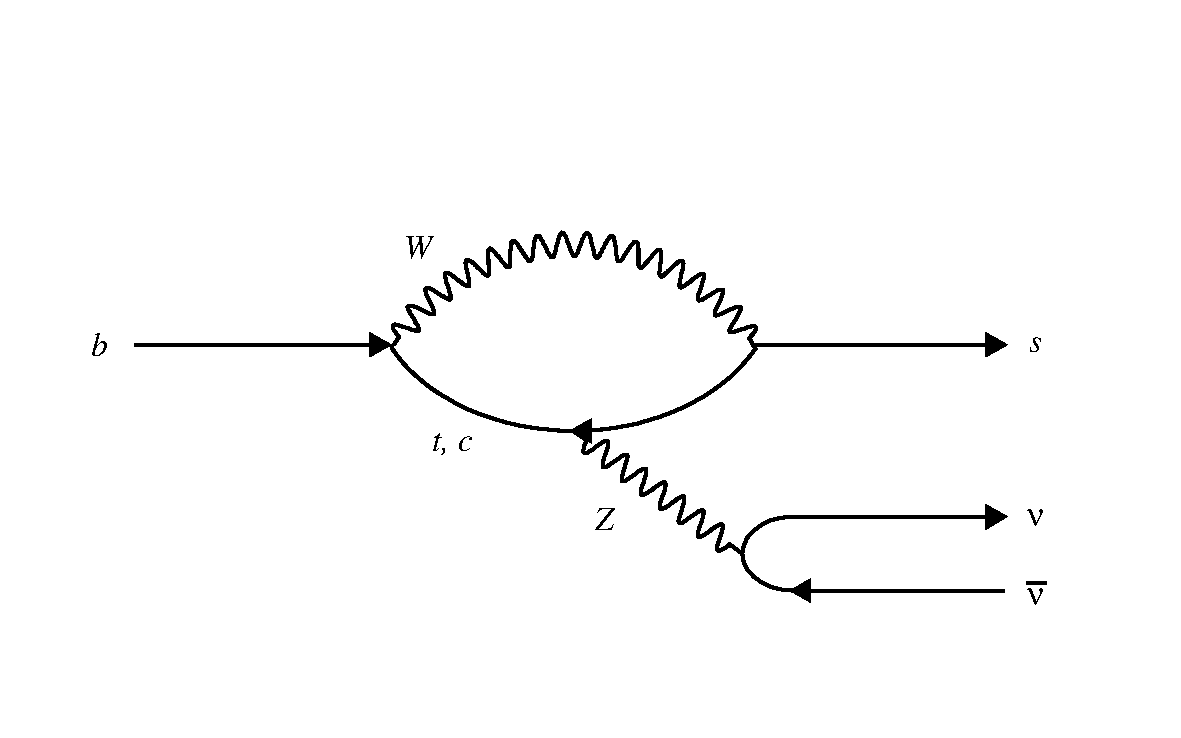
\includegraphics[width=0.45\textwidth]{FeynmanDiagram_hvv_1-eps-converted-to.pdf}
		\label{introduction_figure/FeynmanDiagram_hvv_1}
	}
	\subfigure[]{
		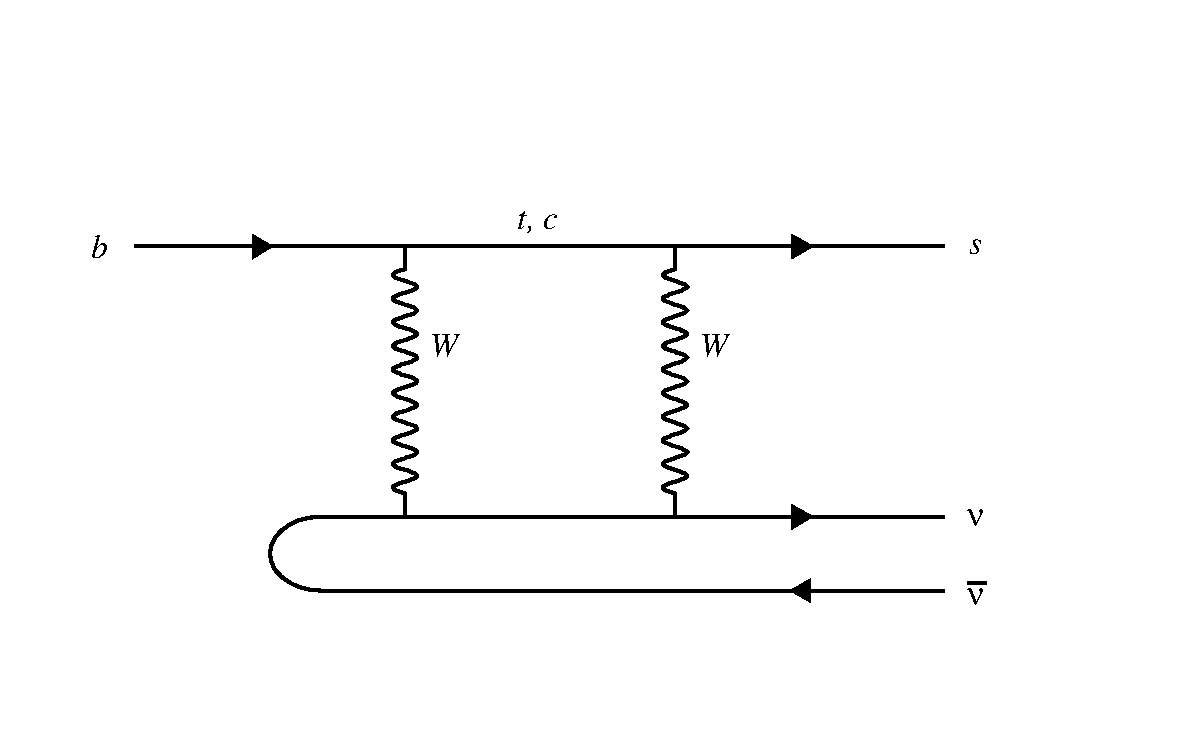
\includegraphics[width=0.45\textwidth]{FeynmanDiagram_hvv_2-eps-converted-to.pdf}
		\label{introduction_figure/FeynmanDiagram_hvv_2}
	}
	
	\caption{Feynman Diagram for $B \rightarrow K^{(*)} \nu \bar{\nu}$ decay }
	\label{FD}	
\end{figure}
\newpage
where
\begin{equation}
\label{eq:smt2}
\mathcal{O}_L = \frac{e^2}{16\pi^2} (\bar{s}\gamma_{\mu}P_L b)(\bar{\nu}\gamma^{\mu}(1-\gamma_5)\nu)
\end{equation}
and $C^{SM}_{L}$ is known as the Wilson coefficient, result in Eq. \ref{eq:smt3}[]
\begin{equation}
\label{eq:smt3}
C^{SM}_{L} = -X_t / s^2_w, ~~~ X_t = 1.469\pm 0.017
\end{equation}
The differential branching ratios as a function of $q^2$, given by [] are


Here, the factor of 3 stems from the total neutrino flavour, $N$ stand for a normalization factor shown in Eq. \ref{eq:smt6}, $\rho_i$ are  rescaled form factors shown in Eq. \ref{eq:smt6} $\sim$ \ref{eq:smt10}.
\begin{equation}
\label{eq:smt6}
N = V_{tb}V_{ts}^*\frac{G_F \alpha}{16 \pi ^2} \sqrt{\frac{m_B}{3 \pi}}
\end{equation}
\begin{equation}
\label{eq:smt7}
\rho_V(q^2) = \frac{2q^2 \lambda^{3/2}_{K^*}(q^2)}{(m_B + m_{K^*})^2 m_B^4}[V(q^2)]^2
\end{equation}
\begin{equation}
\label{eq:smt8}
\rho_{A1}(q^2) = \frac{2q^2 \lambda^{1/2}_{K^*}(q^2)(m_B + m_{K^*})^2}{ m_B^4}[A_1(q^2)]^2
\end{equation}
\begin{equation}
\label{eq:smt9}
\rho_{A12}(q^2) = \frac{64m^2_{K^*}\lambda^{1/2}_{K^*}(q^2)}{m_B^2}[A_{12}(q^2)]^2
\end{equation}
\begin{equation}
\label{eq:smt10}
\rho_K(q^2) = \frac{\lambda^{3/2}_{K}(q^2)}{m_B^4}[f^K_+(q^2)]^2
\end{equation}
which the 
\begin{equation}
\label{eq:smt11}
\lambda (a,b,c) = a^2+b^2+c^2-2(ab+bc+ac), \lambda^{3/2}_{K}(q^2) \equiv \lambda(m^2_B, m^2_K{(*)}, q^2)
\end{equation}
The SM branching ratio estimate to be $\mathcal{B}(B^+ \rightarrow K^{+} \nu \bar{\nu})=\mathcal{B}(B^0 \rightarrow K^{0} \nu \bar{\nu}) = (4.5 \pm 0.7) \times 10^{-6}$, $\mathcal{B}(B^+ \rightarrow K^{*+} \nu \bar{\nu})=\mathcal{B}(B^0 \rightarrow K^{*0} \nu \bar{\nu}) = (6.8 ^{+1.0}_{-1.1}) \times 10^{-6}$.\\

There are many new-physics models predicted that could significantly enhance the branching ratio, as well as modify the expected SM $S_B$ distributions, where $S_B \equiv q^2/m^2_B$, $q^2$ is the square magnitude of missing four-momentum as the neutrino pair, $m_B$ is the B meson mass. Some of these models predict that some massive particle could contribute extra loop diagrams with similar amplitudes as those in SM, like nonstandard $Z^0$ couplings with SUSY(supersymmetric) particle, fourth generation quarks, anomalous top-charm transitions, and a massive U(1) gauge boson $Z^{'}$. There are others thing that can do some contribution, such like the missing part of the nrutrino pair can be replaced as the low-mass dark mass or right-handed neutrino candidate, the kaon can be replaced as the SUSY particles.\\
This analysis $B \rightarrow K^{(*)} \nu \bar{\nu}$ is measure several times by both BaBar and Belle experiment, with the current data, there were no signal observed, but was very close to see it. In this thesis, our goal is to do the enhancement on signal efficiency in the previous study at Belle\cite{ref:Lutz2013}, and do the bin-by-bin optimization on $S_B$ distribution, because certain new-physics models imply that enhancements are possible at high $S_B$ region, instead of removing the low $S_B$ region in the previous study, we measure the partial branching fraction$(\Delta \mathcal{B})$ in the interval of $S_B = 0.1$.\\
We also perform the measurement result in pseudo Belle II data, which times the factor of 50 in both signal Monte Carlo and background Monte Carlo, with the Belle II experiment in the future, the luminosity will increasing by the factor of 50, this gives us the chance to probe the new physics models through such kind of these decay mode like $B \rightarrow K^{(*)} \nu \bar{\nu}$.

\section{Standard Model}
The Standard Model (SM) is a relativistic quantum field theory that describing the interactions between the elementary particle. In Standard Model, four families of the elementary particle and also it antiparticle are include, there are six kinds of quarks, six kinds of leptons, four kinds of gauge bosons and the Higgs boson.The Standard Model is also describes all known forces, electromagnetic force, weak force, and strong force. Only gravity is not include in Standard Model. Figure \ref{Standard_Model_of_Elementary_Particles} shows all the element and their corresponding properties in Standard Model, and Figure \ref{Elementary_particle_interactions} shows the interaction between the elementary particle in SM.\\

\begin{figure}[h]
		\centering
		\subfigure[Standard Model of Elementary Particles.]{
			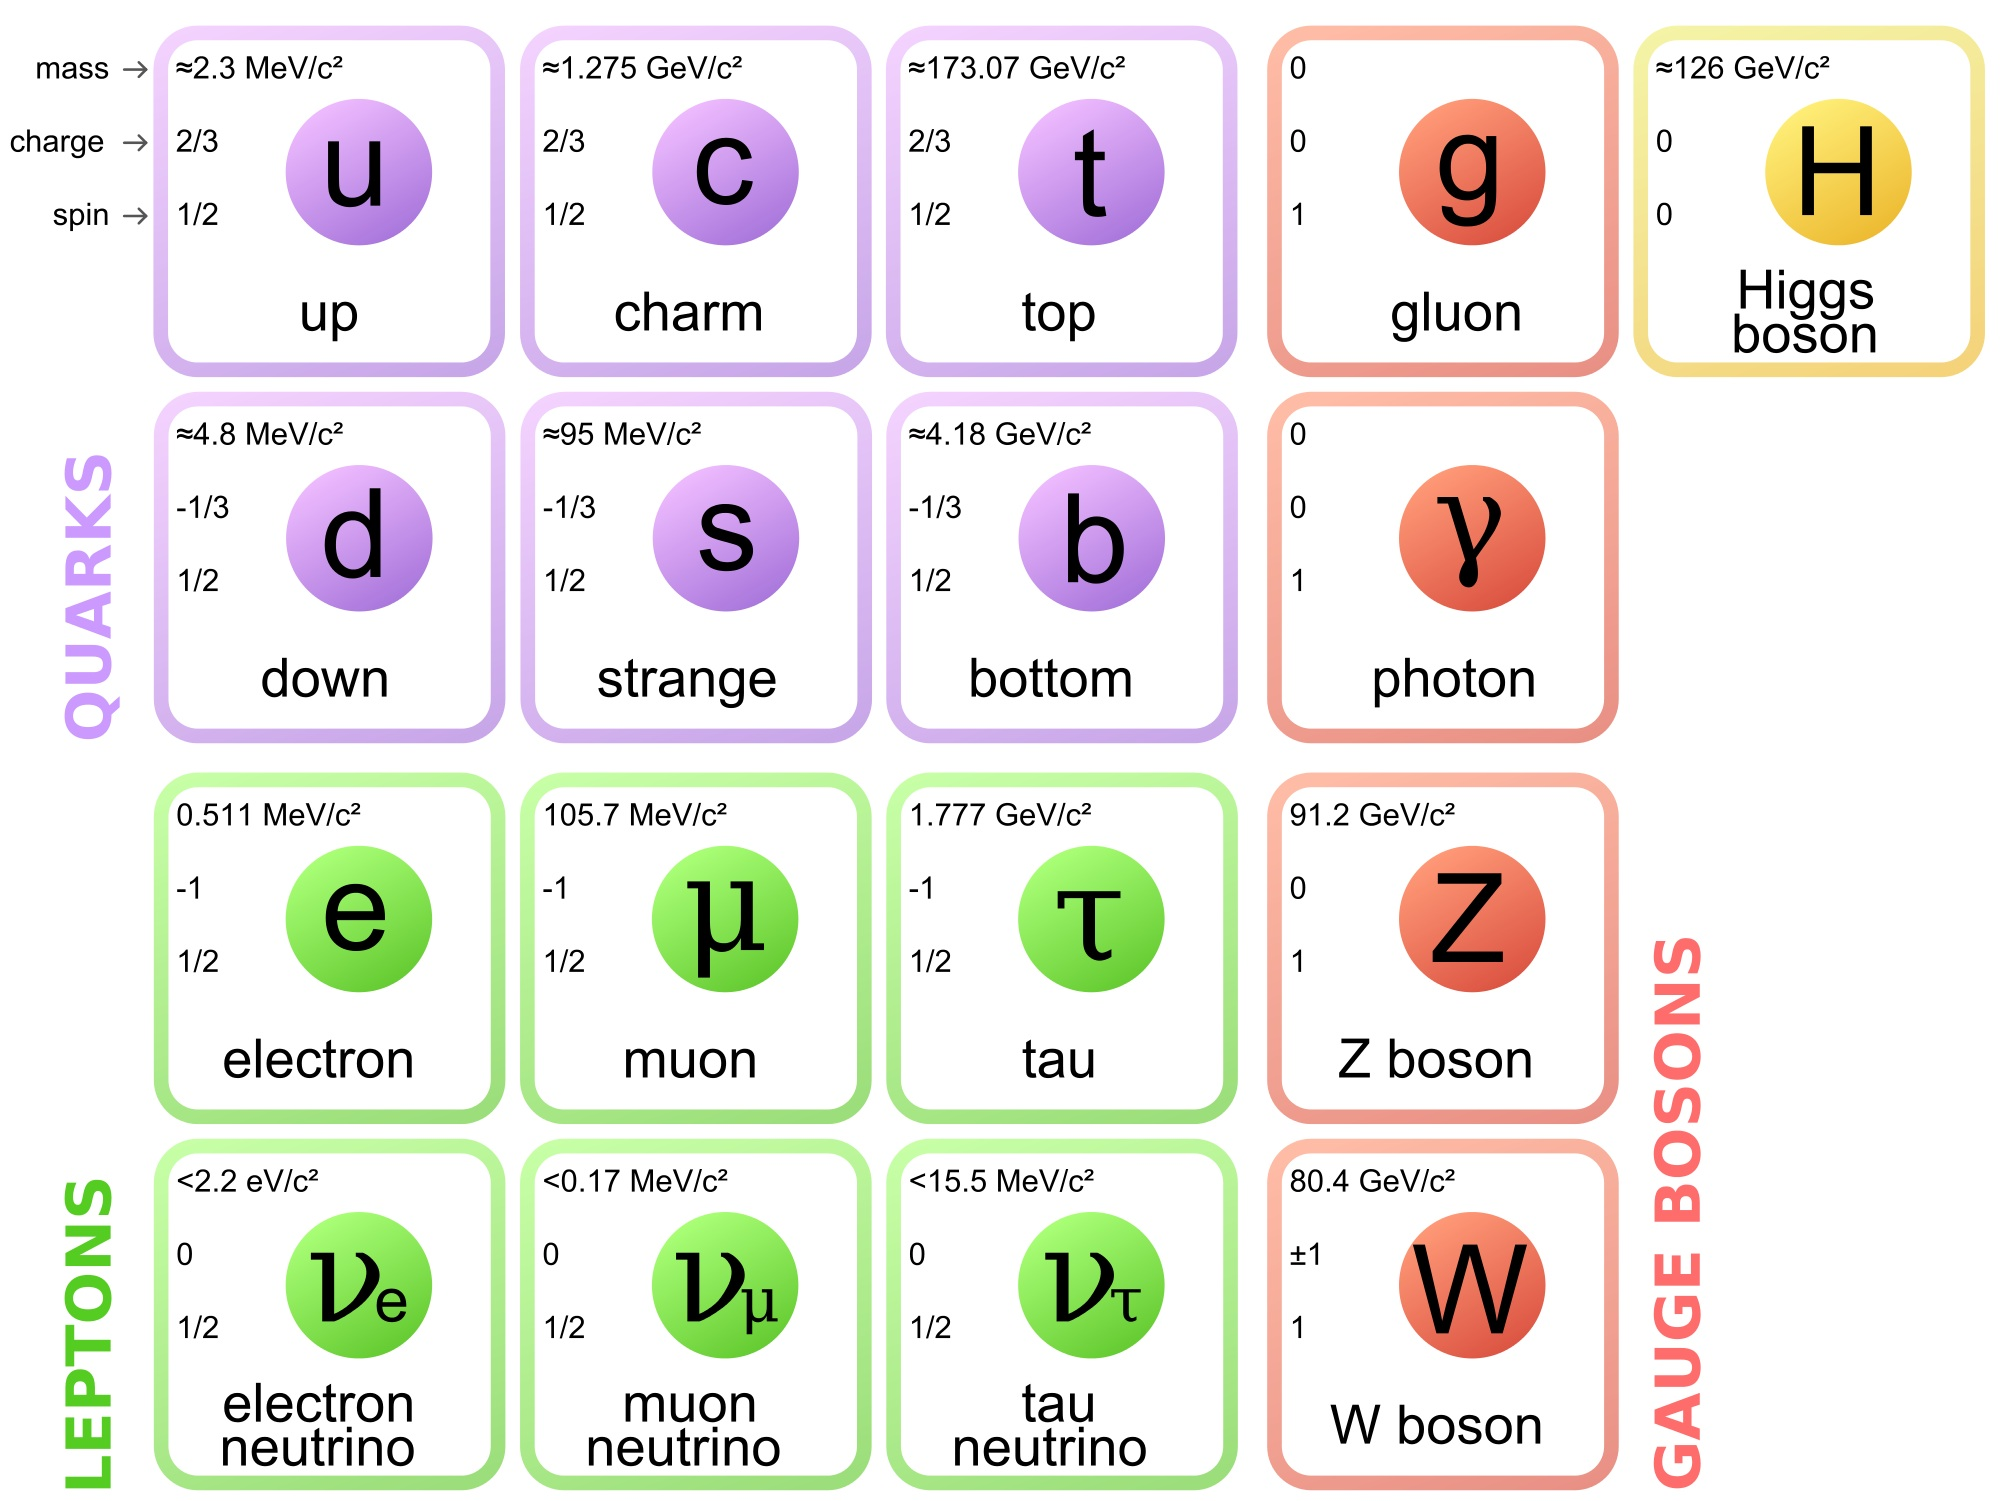
\includegraphics[width=0.45\textwidth]{Standard_Model_of_Elementary_Particles}
			\label{introduction_figure/Standard_Model_of_Elementary_Particles}
		}
		\subfigure[The interactions between elementary particle of the Standard model.]{
			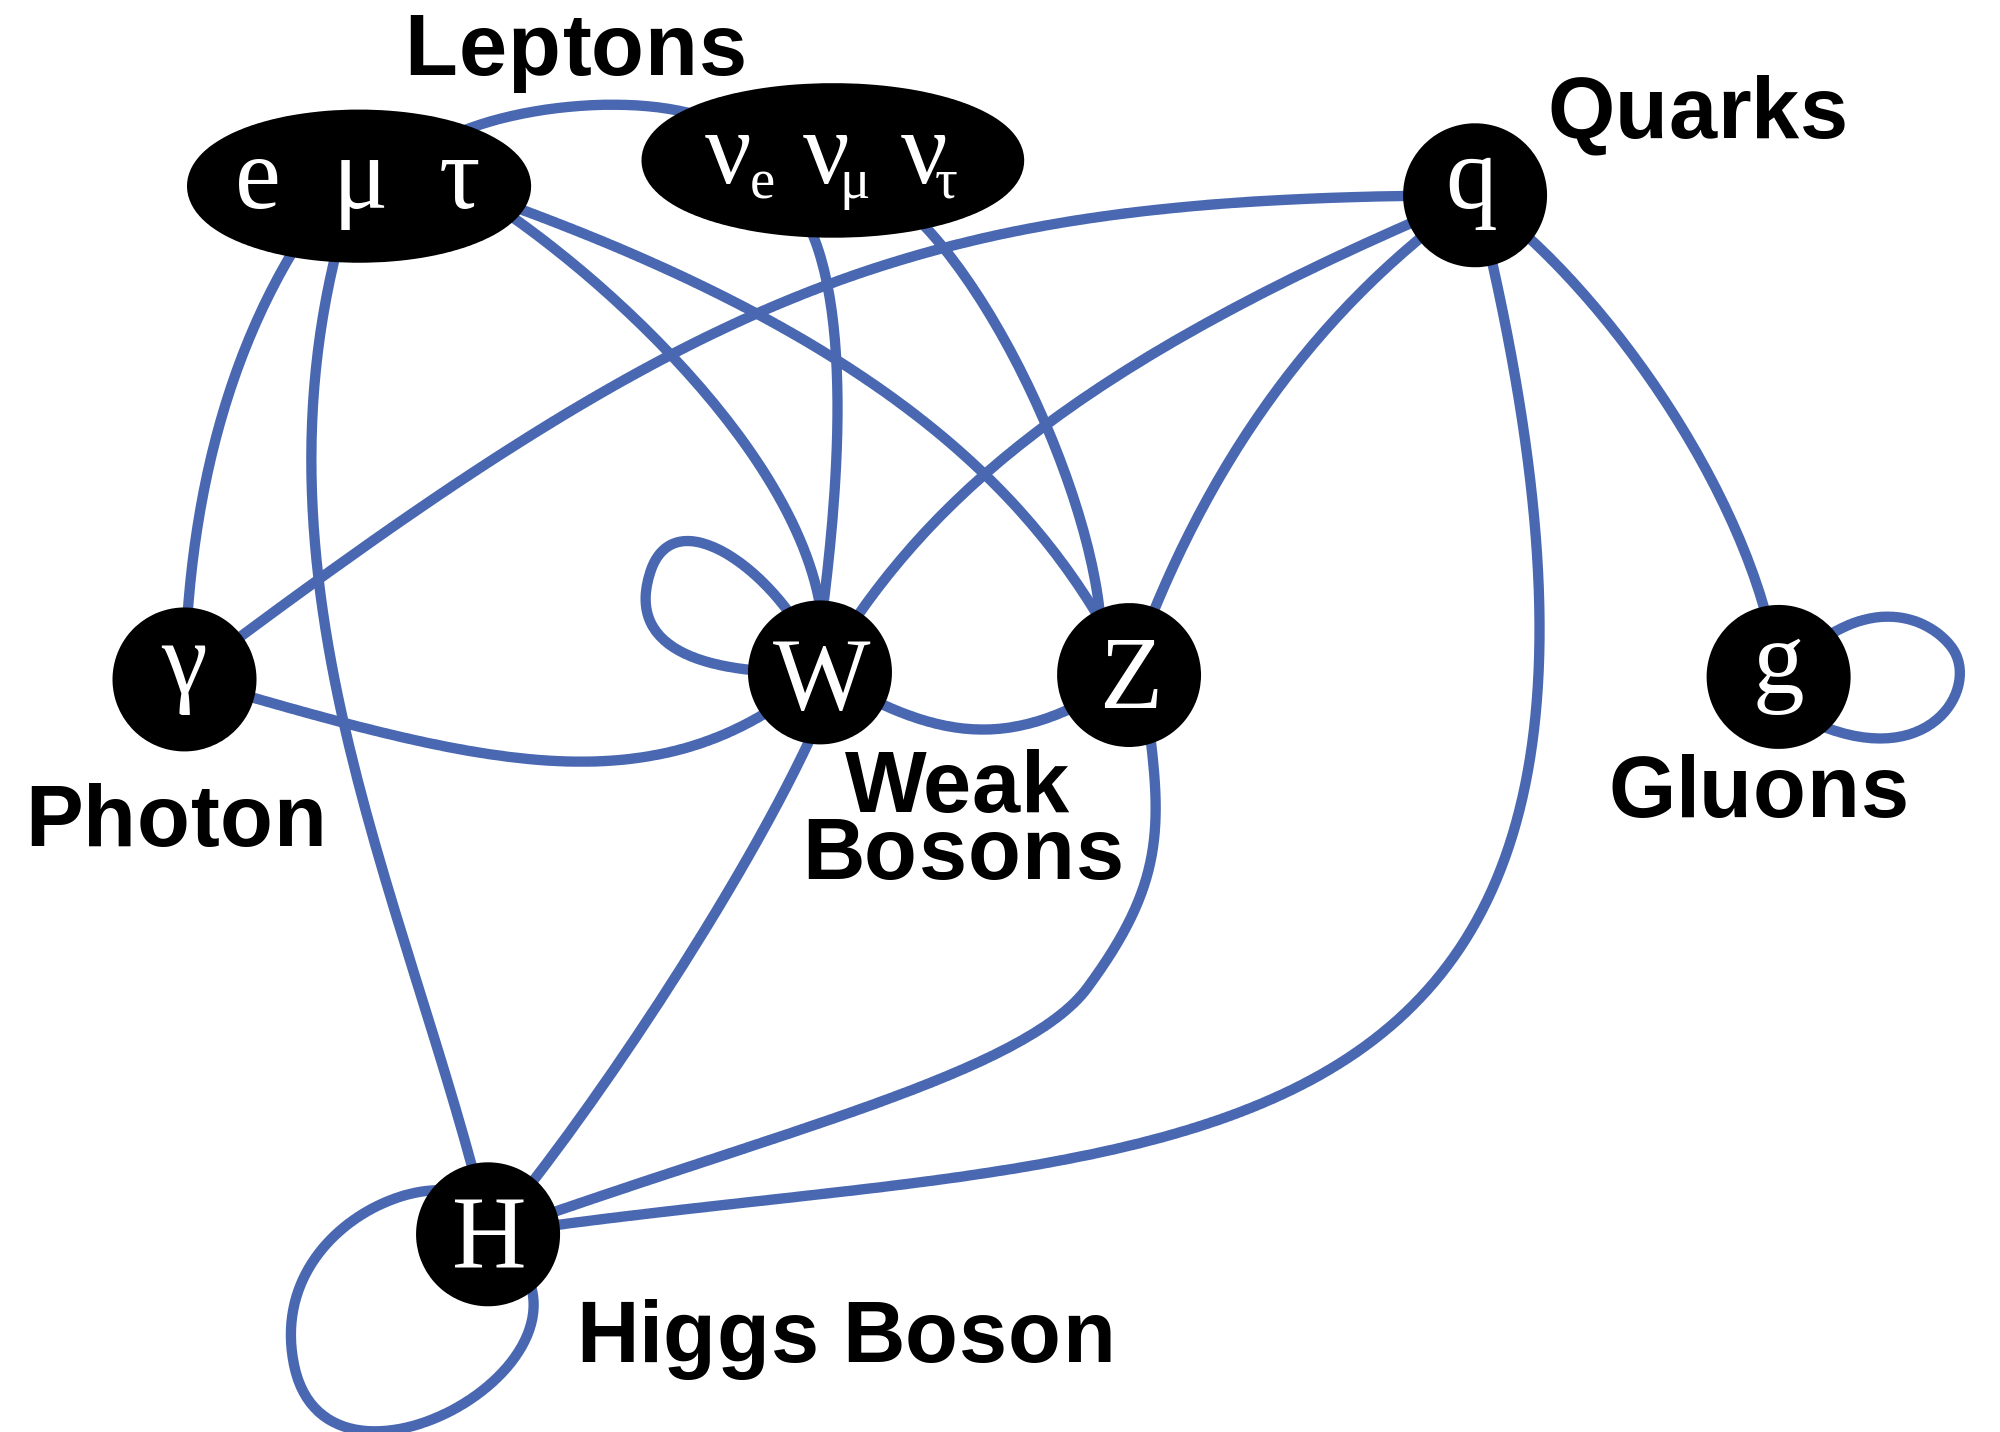
\includegraphics[width=0.45\textwidth]{Elementary_particle_interactions}
			\label{introduction_figure/Elementary_particle_interactions}
		}
		\label{SM}	
		\caption{fuck}

\end{figure}

Mathematically, the Standard Model is formed by the local gauge symmetry $SU$(3) $\times$ $SU$(2) $\times$ $U$(1). The $SU$(3) represents the strong force and only particle can interact strongly, The $SU$(2) is stand for weak interaction, and only the particle in weak doublets can interaction through weak force and electromagnetic force is described by $U$(1) symmetry with the weak hyper-charge.


\subsection{Elementary Particle}
\begin{table}[h]
\begin{center}
\begin{tabular}{l|c|c|c|c|c|c|c|c|r}
\hline
\hline
			Quark   &  Mass(Mev/$c^2$)   	&   J     &    B      &   Q    &    $I_3$   &   T      &   S    &   C   &	$B^{'}$   \\
\hline
			  $u$      & 2.3    	&   1/2     &  +1/3        &   +2/3    &   +1/2    &    0     &   0    &   0   &0	   \\
\hline
			  $d$     &  4.8   	&     1/2    &     +1/3      &   -1/3    &    -1/2   &    0     &   0    &   0   &	0   \\
\hline
			 $c$      &   1275  	&    1/2     &    +1/3       &   +2/3    &   0    &    0     &  0     &  +1    &0	   \\
\hline
			 $s$		&  95   	&   1/2      &    +1/3       &   -1/3    &   0    &    0     &   -1    &    0  &0	   \\
\hline
			 $t$		&   173210  	&   1/2      &   +1/3        &   +2/3    &  0     &   +1      &   0    &  0    &0	   \\		
\hline
			 $b$		&  4180   	&   1/2      &     +1/3      &   -1/3    &  0     &     0    &   0    &  0    &	-1   \\		
\hline
\hline						        
\end{tabular}
\caption{ Some quantum number of the six quarks\\J = total angular momentum, B = baryon number, Q = electric charge, I3 = isospin, C = charm, S = strangeness, T = topness, B′ = bottomness.} \label{t:quarka}
\end{center}
\end{table}

\subsection{The Cabibo-Kobayashi-Maskawa Matrix}


\subsection{B physics}
In 1977,the third generation bottom quark(b) was observed by the CFS\footnotemark[1]
E288 experiment headed by Leon Lederman at Fermi lab. 
A dimuon resonance at 9.5 GeV was found,which now recognized as $\Upsilon$ (1S).
$\Upsilon$ is a flavorless meson formed by a b quark and an anti-b quark. Figure 1.3 shows
the cross section to particle production of various $\Upsilon$ states measured by CUSB$\footnotemark[2]$
and CLEO detector in CESR$\footnotemark[2]$ at Cornell University.
B mesons are the
\footnotetext[1]{Columbia-Fermilab-Stony Brook colla}
\footnotetext[2]{Ego's id is mapped by Appendix}
\subsection{CP Violation}

%\begin{table}[t]
%\begin{center}
%\begin{tabular}{lcc}
%
%\hline
%                    &  {\small Itti's method}     & {\small Fuzzy growing}    \\
%\hline
%{\small Precision}           &  0.4475    & 0.4506 \\
%{\small Recall}              &  0.5515    & 0.5542 \\
%\hline
%
%\end{tabular}
%\caption[Evaluation of FOA sets]{\small Evaluation of FOA sets. } \label{t:FOA}
%\end{center}
%\end{table}

%\chapter{Belle Experiment}
\section{Introduction to the Belle Experiment}
The Belle experiment is designed to study the physics of CP violation,
which holds the key to the origin of universe. It is conducted by the Belle collaboration,
an international collaboration of physicists and engineers from 16 countries,
located at the High Energy Accelerator Research Organization(KEK) in Tsukuba, Ibaraki Prefecture,Japan.
This big project includes two major facilities: the KEKB accelerator and the Belle detector. Figure 2.1 shows
the bird's eye view of the organization.
%\include{}
\section{The KEKB Accelerator}
KEKB[29,30], which stands for the KEK B-factory,is an asymmetric energy
\section{The Belle Detector}
%\chapter{Event Selection and Reconstruction}
\section{Data Sample}
In this analysis, we use the full data which was collected by the Belle detector at the KEKB asymmetric-energy $e^+e^-$ colider\
(with one side is 3.5 GeV and another is 8GeV).The data on the $\Upsilon(4S)$ resonance is used, with the integrated luminosity is 710 $fb^-1$.\
The total number of $B\bar{B}$ event from experiment 7 to 65 is $771.581\pm10.566$ million. 
\subsection{Monte Carlo sample}
And there are various officially produced Monte Carlo have been used in the analysis, There are generic, continuum and rare MC. \
The generic Monte Carlo is about the decay of B mesons where b quark decay into a c quack, and the sample include two kinds, one is called "charged", which refer to the decay of\
 $\Upsilon(4s)$ into $B^+ B^-$ pairs, the other is called "mixed", which refer to the decay of $\Upsilon(4s)$ into $B^0 \bar{B^0}$ pairs.There are ten streams of generic MC available totally\
corresponding to ten times of Belle I data size.In this study, six stream of generic MC are used for now.Another kind of MC sample is the continuum, where the events have no $\Upsilon(4s)$ been\
produced, and the corresponding processes are $e^+ e^-$ pair decay to $u, d, s, c$ quark pairs, There are six streams of continuum MC available totally. All six streams of the continuum MC sample\
are used in this study.The other is rare MC sample which cover all the non $b \rightarrow c$ B decay transitions. The rare MC sample contain the 50 times the data luminosity\
for $b \rightarrow u \ell \nu$ transition, and 20 times data size for all other non $b \rightarrow c$ channel.\\
For signal decay study, all signal sample with $B \rightarrow K^{(*)} \nu \bar{\nu}$ which $K^{(*)}$ is stand for are generated with EvtGen package, and detector simulation is done with GEANT package.\
In the decay generated process, model VSS is used to simulate $\Upsilon(4s)$ decay $B^+ B^-$ and model VSS\_BMIX dm is used to simulate $\Upsilon(4s)$ decay $B^0 \bar{B^0}$ with $B^0 \bar{B^0}$\
mix condition turn on.The $B \rightarrow K^{(*)} \nu \bar{\nu}$ for all $K$ channel are used phase space decay model to describe.There are 771,0000 signal MC sample used for each $K{(*)}$ channels.\
%\subsection{Blind Analysis}
\section{Event Selection}
In this study, we only consider events passed through both HadronB(J) skim and full reconstruction skim.
Candidate $e^+ e^- \rightarrow \Upsilon(4s) \rightarrow B B $ events are characterized by a fully reconstructed tag-side \
B meson. The remaining particles are assumed to be products of signal-side B meson.
\subsection{Hadronic Tag}
In order to study the mode which include missing particle, e.g., neutrinos, We reconstruct the hadronic B meson, which called $B_{tag}$ by using the Fullrecon package in Belle library.The latest version Fullrecon package with the Neurobayes neural networks\cite{ref:Feindt2011} have the better performance on the candidate selection, and also increase the purity and efficiency that compare to the old Fullrecon package. \
The $B_{tag}$ candidates can reconstructed in one of the following mode:\\
$B^0 \rightarrow D^{(*)-} \pi^+ $ , $ D^{(*)-} \rho^+$ , $ D^{(*)-}a^+_1$ , $ D^{(*)-} D^{(*)+}_s$ ,etc.\\
$B^+ \rightarrow\bar{D}^{(*)0} \pi^+$ , $ \bar{D}^{(*)0} \rho^+$ , $ \bar{D}^{(*)0}a^+_1$ , $ \bar{D}^{(*)0} D^{(*)+}_s$ ,etc.\\
$D$ meson can reconstructed by:\\
$D^- \rightarrow K^0_s \pi^- \pi^0$ , $K^0_s \pi^- \pi^+ \pi^-$ , $K^+ \pi^+ \pi^-$ , $K^+  \pi^- \pi^-\pi^0$ ,etc. \\
\vspace*{1mm}
$\bar{D^0} \rightarrow K^+ \pi^-$ , $K^+ \pi^- \pi^0$ , $K^+ \pi^- \pi^+ \pi^-$ , $K^0_s \pi^0$ , $K^0_s \pi^- \pi^+$ , $K^0_s \pi^- \pi^+ \pi^0$ , $K^- K^+$ ,etc. \\
\vspace*{1mm}
$D^{*-}(D^*0) \rightarrow \bar{D^0} \pi^-(\bar{D^0} \pi^0$ , $ \bar{D^0} \gamma)$ ; $D^{*+}_s \rightarrow D^+_s \gamma$ ; $D^+_s \rightarrow K^0_s K^+$ and $K^+ K^- \pi^+$ .\\
\vspace*{2mm}
There are totally 1104 hadronic decay channels include. \
For the $B_{tag}$ candidate selection, choose the best candidate by using the event-wide rank according to NeuroBayes output with continuum suppression(cont\_NBRank).We also reject events with wrong sign reconstruction best $B_{tag}$\
will be rejected. i.e., reject the event of the signal side $B^+ \rightarrow K^+ \nu \bar{\nu}$ with the best $B_{tag}$ candidate $B^0$.  

\subsection{Particle Selection Criterion}
\begin{itemize}[leftmargin=*]
\item \textbf{Track Selection}\\
The track particles are all collected from MDST\_CHARGED bank after forming a $B_{tag}$, we require the transverse momentum $p_t$ greater than 0.1 GeV/c, and also require the impact parameter in radial direction\
$|dr| <$ 2cm, and in beam direction $|dz| <$ 5cm.
\item \textbf{Charge Particle Identification}\\
\textbf{$\bm{K^\pm}$ candidates} of the particle identification likelihood ratio $\mathcal{L}_{ K \pi}$ > 0.6,  $\mathcal{L_{\mu}}$ < 0.9\\
and  $\mathcal{L}_{e}$ < 0.9. \\
\textbf{$\bm{\pi^\pm}$ candidates} of the particle identification likelihood ratio $\mathcal{L_{ K \pi}}$ < 0.4,  $\mathcal{L_{\mu}}$ < 0.9\\
and  $\mathcal{L}_{e}$ < 0.9.\\
\textbf{$\bm{e^\pm}$ candidates} of the particle identification likelihood ratio $\mathcal{L}_{e}$ > 0.9, and also require \\
$\mathcal{L_{\mu}}$ < 0.9.\\
\textbf{$\bm{\mu^\pm}$ candidates} of the particle identification likelihood ratio $\mathcal{L_{\mu}}$ < 0.9.
\item \textbf{$\bm{K_s}$ candidates selection}\\
The $K_s$ candidates are all collected from MDST\_Vee2 bank, require \\ 
goodks == 1, $m_{Ks} > 0.4826$ and $m_{Ks} < 0.5526$ and also the $\chi ^2$ given by Vee2 bank must < 100.
\item \textbf{$\bm{\pi^0}$ candidates selection}\\ 
the $\pi0$ candidates are collected from MDST\_pi0 bank, $\pi^0$ are reconstructed by two photon candidates with an energy of 50MeV at least, \
The invariant mass of the photon pair should be within 117.8$MeV/c^2$ and 150.2$MeV/c^2$.

%and asymmetry $\alpha = \frac{|E_{\gamma1}−E_{\gamma2} |}{|E_{\gamma1}+E_{\gamma2} |}$ is smaller than 0.9.

\item \textbf{$\bm{K_L}$ candidates selection}\\
Collected from MDST\_klong, the $K_L$ candidates have to survive more than two KLM layers.
\item \textbf{$\bm{K^{*\pm}}$ candidates} are reconstructed in two different mode, there are $K^{*\pm} \rightarrow K^\pm \pi^0$ and $K^{*\pm} \rightarrow K_s \pi^\pm$. \
The $K^{*\pm}$ mass have to within the window, 0.8166 < $m_{K^*}$ < 0.9666. , and $K^{*0}$ mass have to within the window, 0.8166 < $m_{K^*}$ < 0.9666.
\item \textbf{$\bm{K^{*0}}$ candidates} are reconstructed in a charge K and a $\pi$. Their invariance mass must within the window 0.8211 < $m_{K^*}$ < 0.9711. \
The invariance mass distribution of
$K^{*0}$, $K^{*\pm}\rightarrow K^\pm \pi^0 $ and $K^{*\pm} \rightarrow K_s \pi^\pm$ are shown in Fig. \ref{K0mass}, \ref{kpi0mass} and \ref{kspimass} respectively.
\end{itemize}

\begin{figure}[h]
	\centering
	\subfigure[$K^{*0}$ mass.]{
		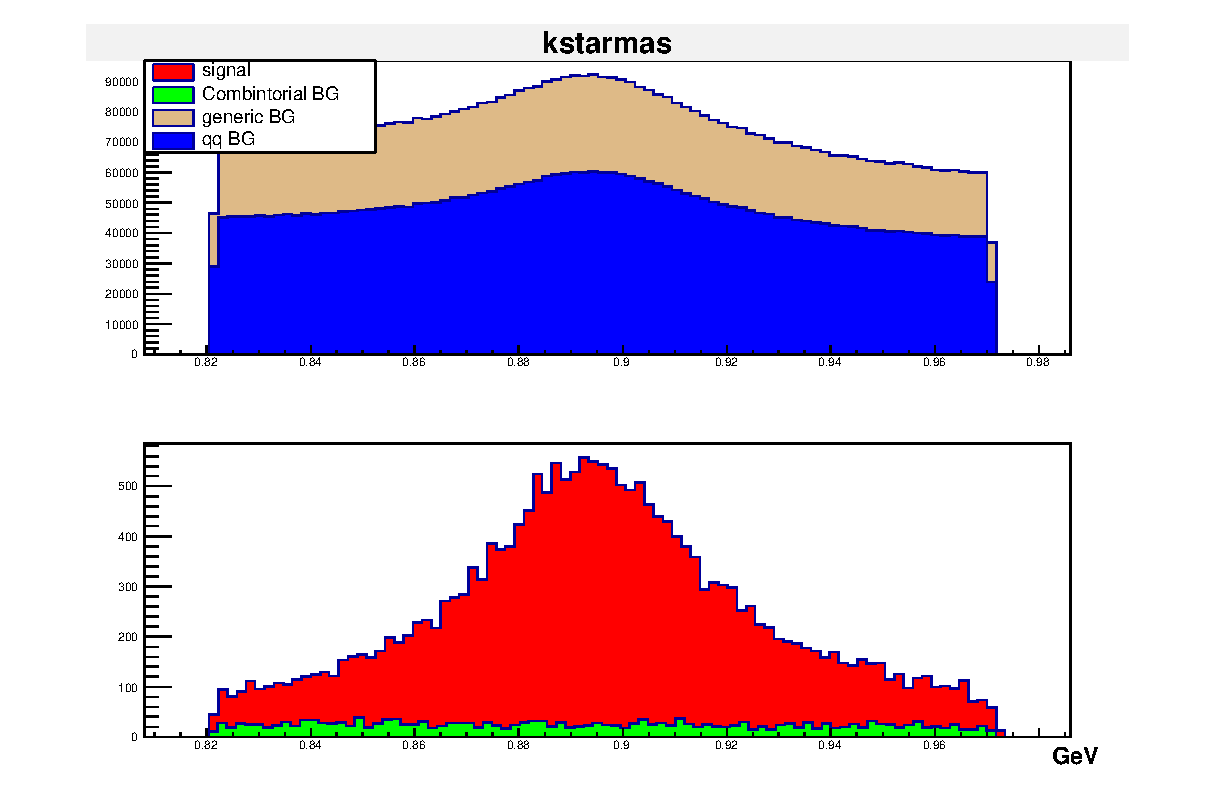
\includegraphics[width=0.45\textwidth]{eventselection_figure/kstarmas_1025_1_b0kst.eps}
		\label{K0mass}
	}
	\subfigure[$K^{*\pm} \rightarrow K^\pm \pi^0$ mass.]{
		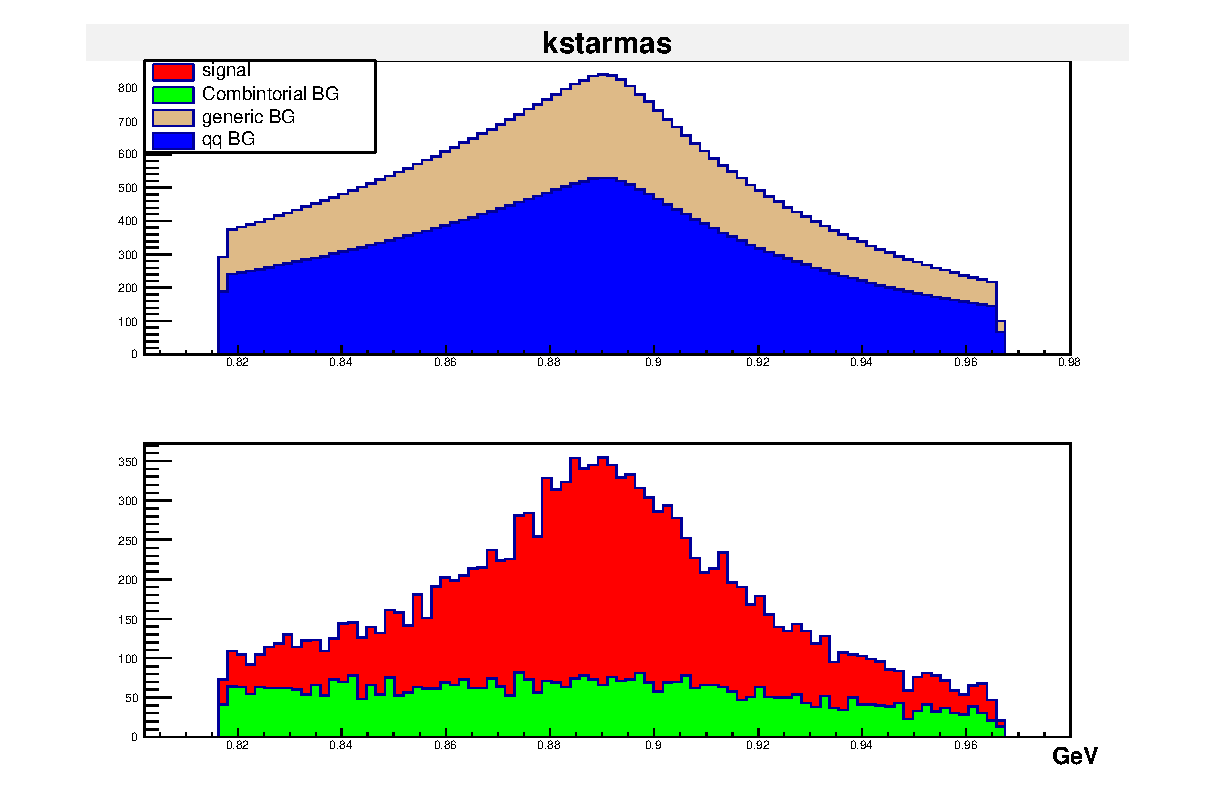
\includegraphics[width=0.45\textwidth]{eventselection_figure/kstarmas_1025_1_kpi0.eps}
		\label{kpi0mass}
	}
	\subfigure[$K^{*\pm} \rightarrow K_s \pi^\pm$ mass.]{
		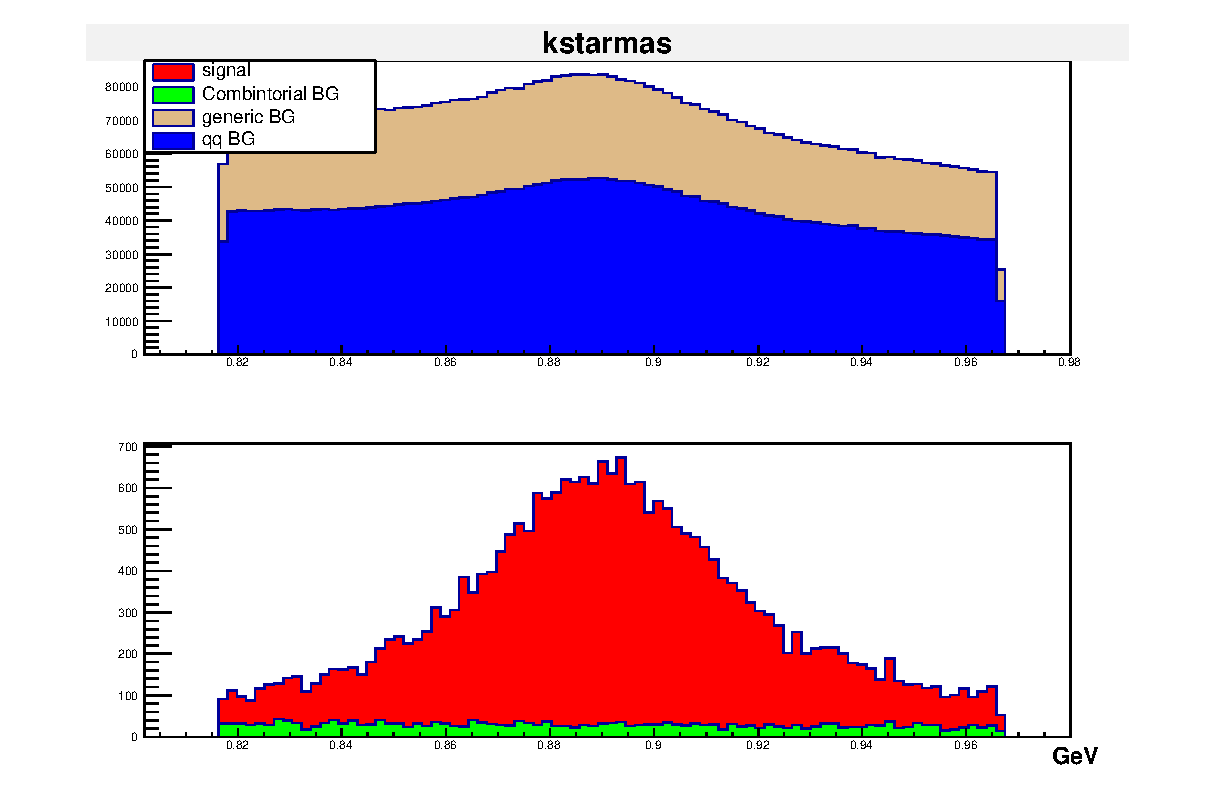
\includegraphics[width=0.45\textwidth]{eventselection_figure/kstarmas_1025_1_kspi.eps}
		\label{kspimass}
	}
	\label{kstarmass}	
	\caption{$K^*$ mass, red represent signal, green represent the combinatorial background,  brown represent the generic background and blue represent continuum background.}
\end{figure}

\subsection{Basic Selection}
It is necessary to apply the basic selection to get rid of the obvious background before we do the Neural-Network bases analysis. This pre-cut can improve the efficiency of \
training result.
\begin{itemize}[leftmargin=*]
\item \textbf{$\bm{B_{tag}}$ selection}\\
The $B_{tag}$ candidates are require to match $M_{bc}$ > 5.24 GeV/$c^2$ and $|\Delta E|$ < 0.05 GeV, the loose requirement on tag side $M_{bc}$ and $|\Delta E|$. \
We also require the $\bm{O_{tag}}$ with continuum suppression, we make a lower cut on log($o_{tag}$) > -7. The distribution of tag-side $M_{bc}$, $|\Delta E|$ and $O_{tag}$ are shown in Fig. \ref{fig:tagbmbc}, \ref{fig:tagbde} and \ref{fig:nbout} respectively.
\item $\bm{E_{ecl}}$\\
$E_{ecl}$ is the total remaining energies of the cluster in ECL detector which are not associated with $B_{tag}$ daughter particle and signal visible candidate.We make the different thresholds on different part of ECL, there are:
\begin{itemize}[leftmargin=*]
\item $E_{cluster}$ > 0.05GeV on barrel.
\item $E_{cluster}$ > 0.10GeV on forward end-cap.
\item $E_{cluster}$ > 0.15GeV on backward end-cap.
\end{itemize}
We define that $E_{ecl}$ < 0.3 GeV as the signal region, $E_{ecl}$ > 0.45 GeV as the sideband region, and set the upper cut on $E_{ecl}$ < 2 GeV.The $E_{ECL}$ distribution are shown in Fig. \ref{fig:sumecl}.
\item \textbf{Veto}\\
We expect there are nothing left beside the $B_{tag}$ and signal-side $B_{sig}$ candidate, we veto the events which have the additional track and also require there are no \
$K_L$ candidates left. We do not require the $\pi^0$ veto, because it'll drop too much signal efficiency. Instead make a $\pi^0$ veto, we make it as the training variable for NeuroBayes.\\
The efficiency table for each mode is shown in table \ref{t:efficiency_k} to \ref{t:efficiency_ks}.
\end{itemize}
\begin{figure}[ht]
	\centering
	\subfigure[$K^{\pm}$ mode.]{
		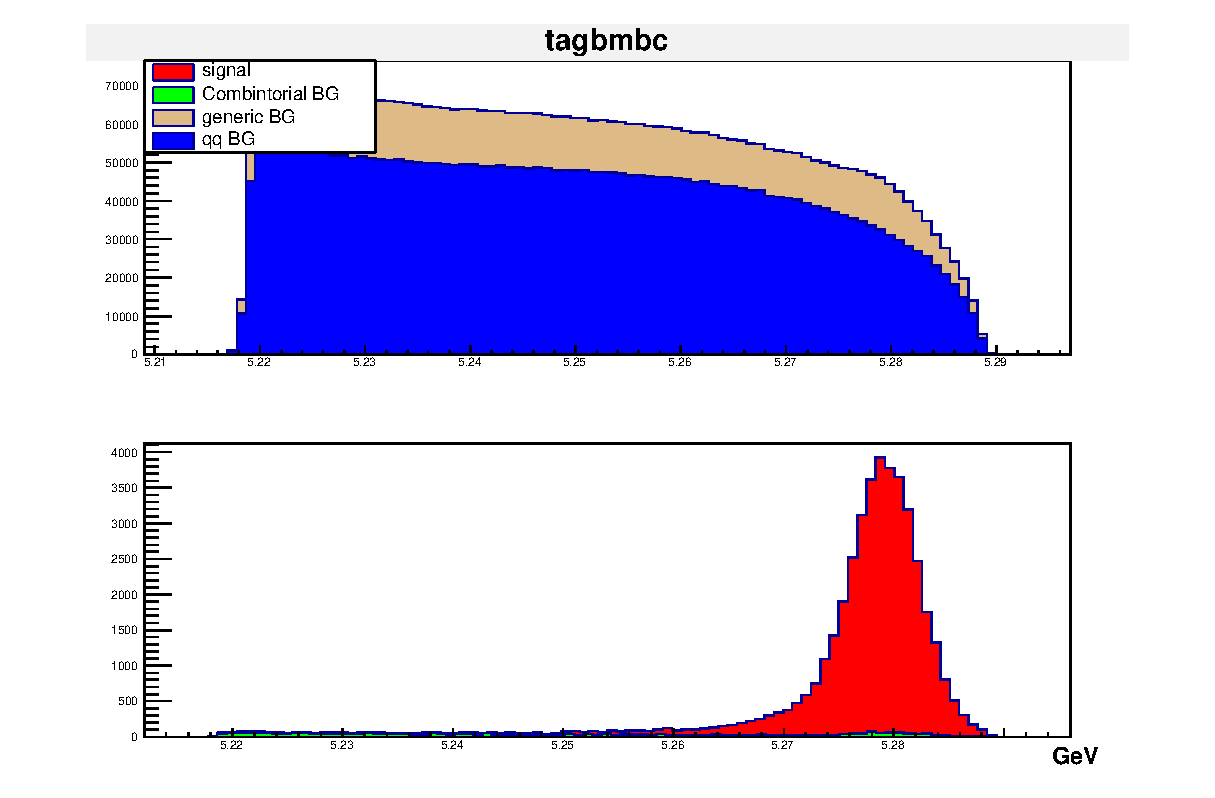
\includegraphics[width=0.45\textwidth]{eventselection_figure/tagbmbc_1025_1.eps}
		\label{kmbc}
	}
	\subfigure[$K^{*\pm} \rightarrow K^\pm \pi^0$ mode.]{
		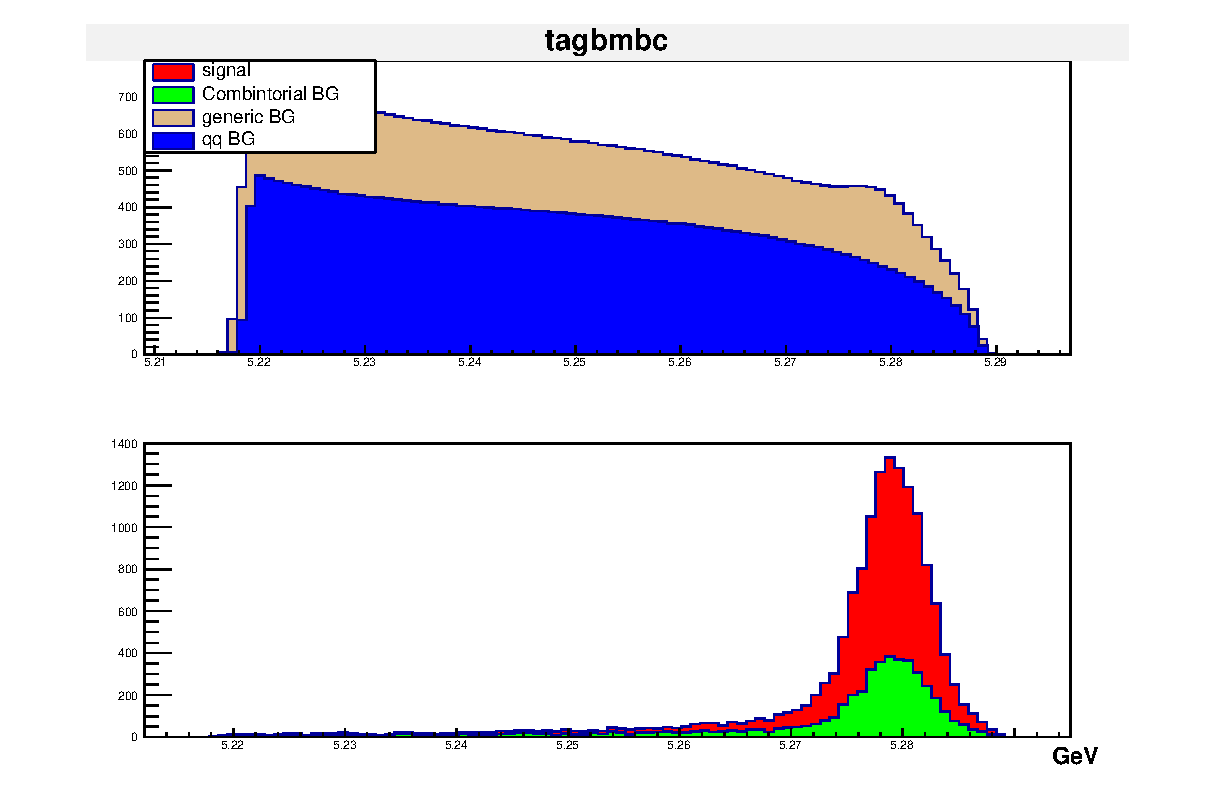
\includegraphics[width=0.45\textwidth]{eventselection_figure/tagbmbc_1025_1_kpi0.eps}
		\label{kpi0mbc}
	}
	\subfigure[$K^{*\pm} \rightarrow K_s \pi^\pm$ mode.]{
		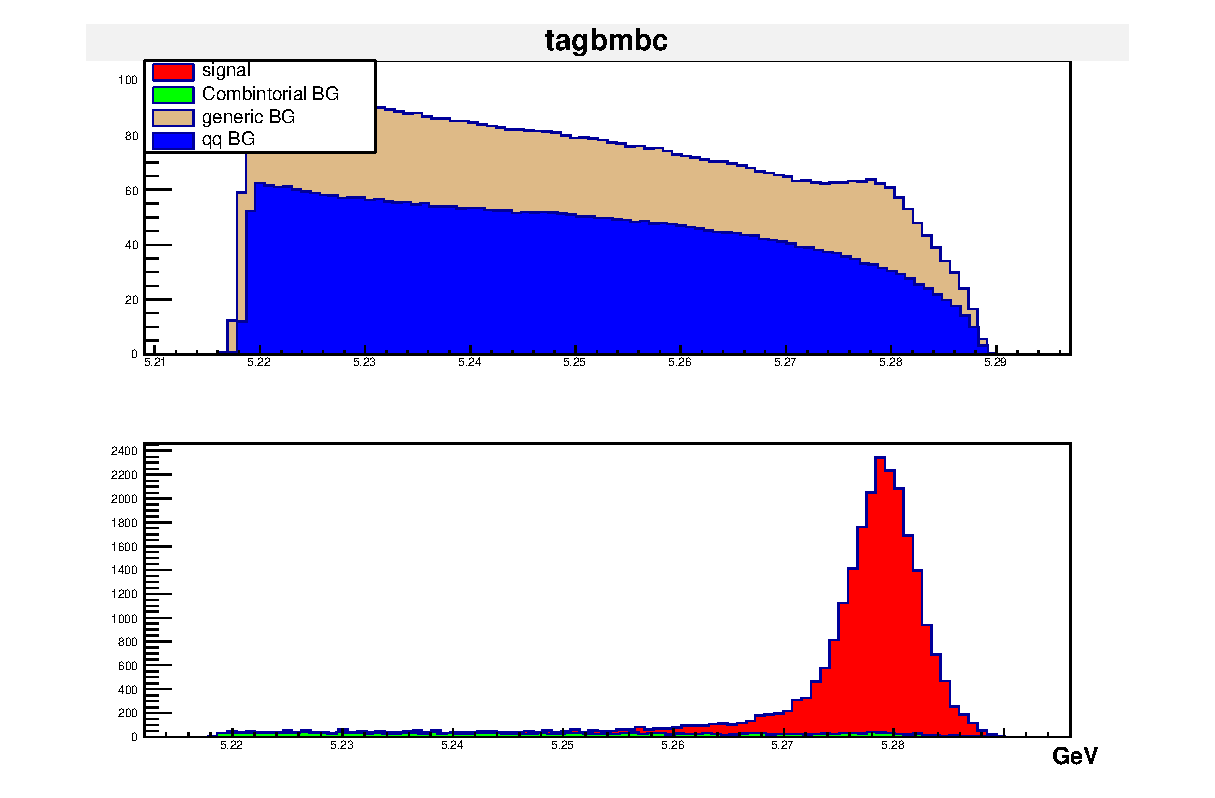
\includegraphics[width=0.45\textwidth]{eventselection_figure/tagbmbc_1025_1_kspi.eps}
		\label{kspimbc}
	}
    \subfigure[$K^{*0}$ mode.]{
		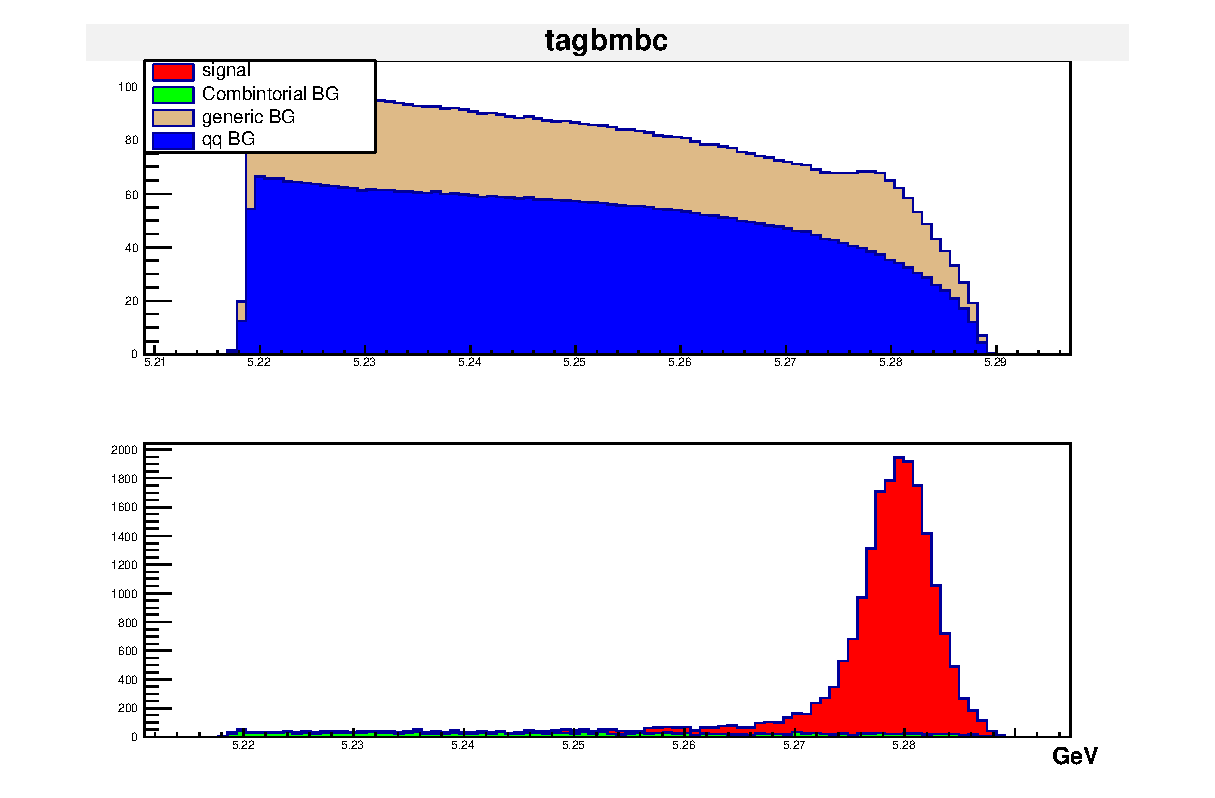
\includegraphics[width=0.45\textwidth]{eventselection_figure/tagbmbc_1025_1_b0kst.eps}
		\label{k0mbc}
	}
    \subfigure[$K_s$ mode.]{
		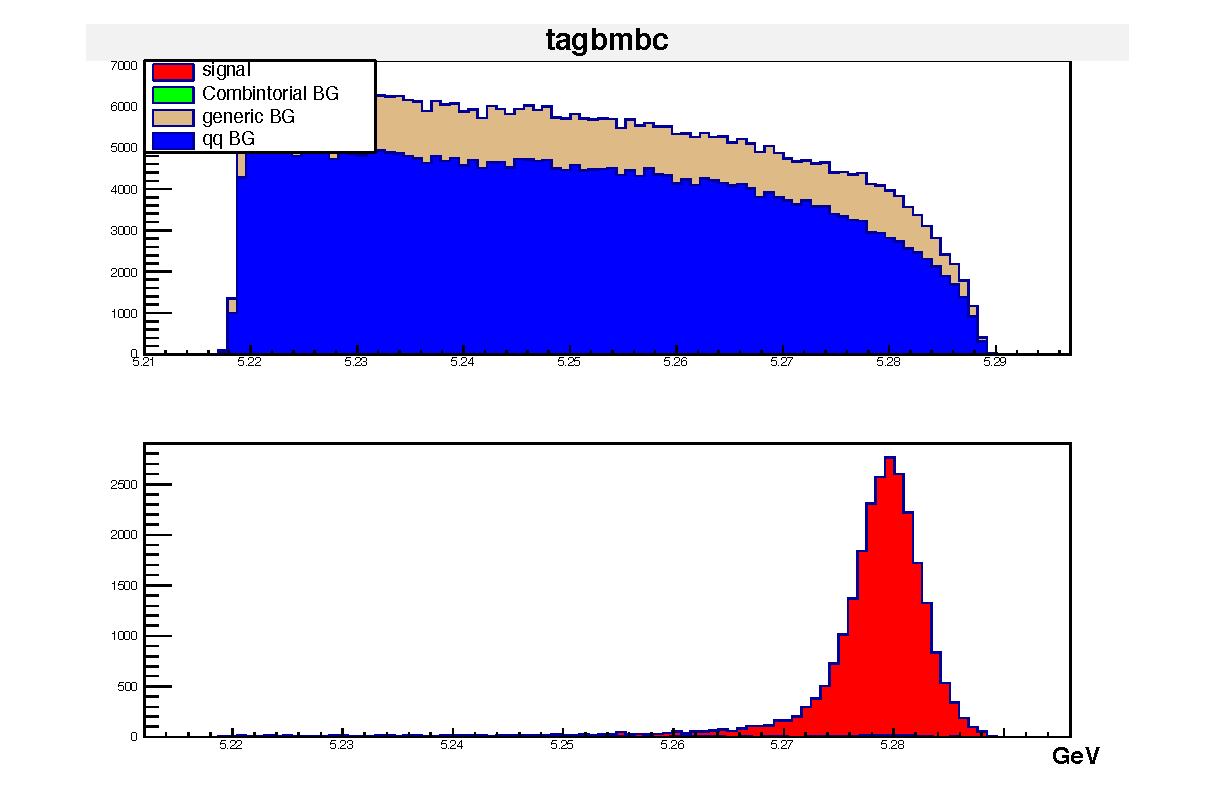
\includegraphics[width=0.45\textwidth]{eventselection_figure/tagbmbc_1025_1_b0ksh.eps}
		\label{ksmbc}
	}
	\caption{Tad-side $M_{bc}$ distribution for each mode. Red represent signal, green represent the combintorial background,  brown represent the generic background and blue represent continuum background.}
    	\label{fig:tagbmbc}	
\end{figure}


\begin{figure}[ht]
	\centering
	\subfigure[$K^{\pm}$ mode.]{
		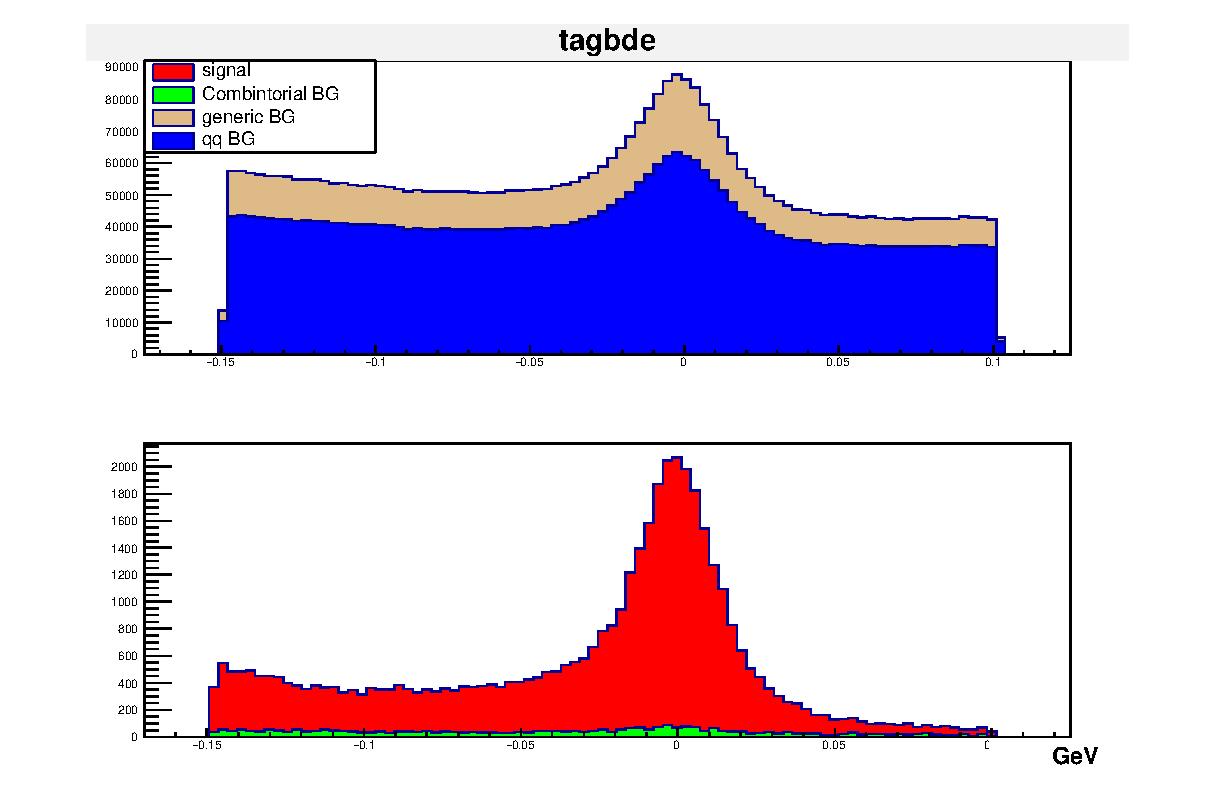
\includegraphics[width=0.45\textwidth]{eventselection_figure/tagbde_1025_1.eps}
		\label{kde}
	}
	\subfigure[$K^{*\pm} \rightarrow K^\pm \pi^0$ mode.]{
		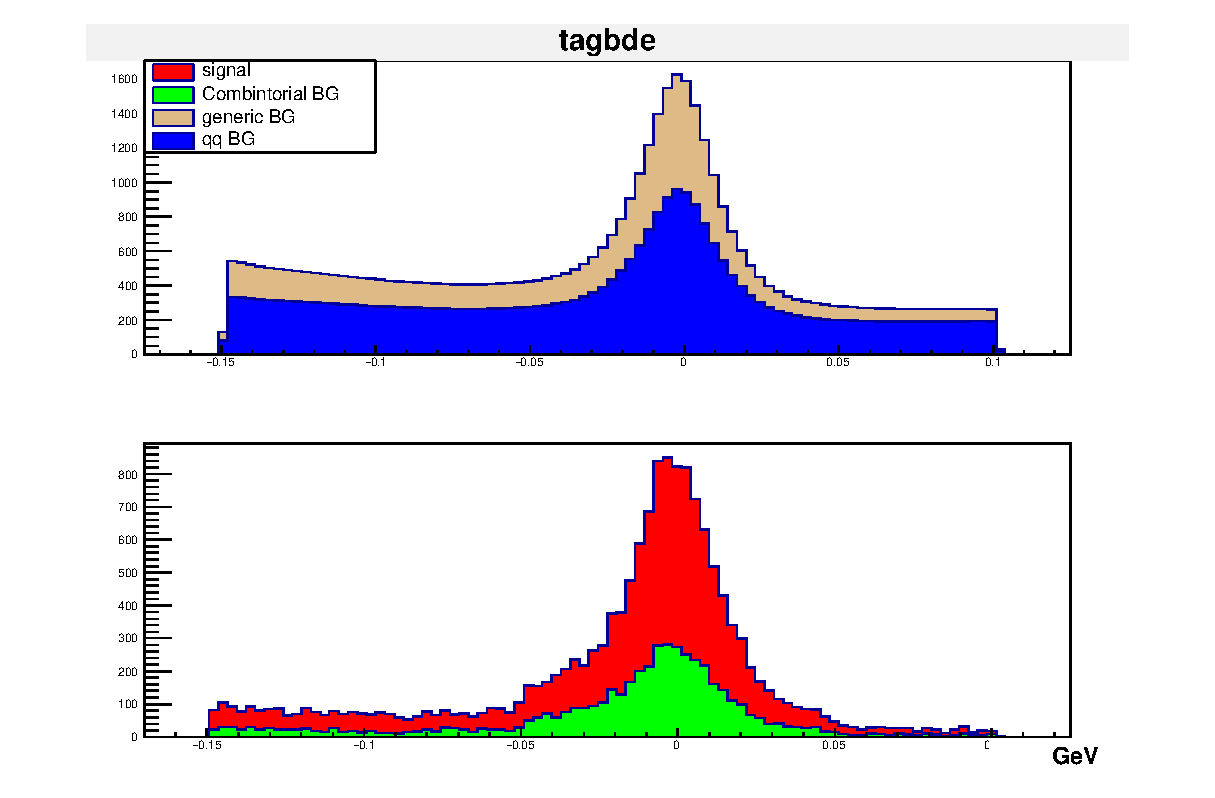
\includegraphics[width=0.45\textwidth]{eventselection_figure/tagbde_1025_1_kpi0.eps}
		\label{kpi0de}
	}
	\subfigure[$K^{*\pm} \rightarrow K_s \pi^\pm$ mode.]{
		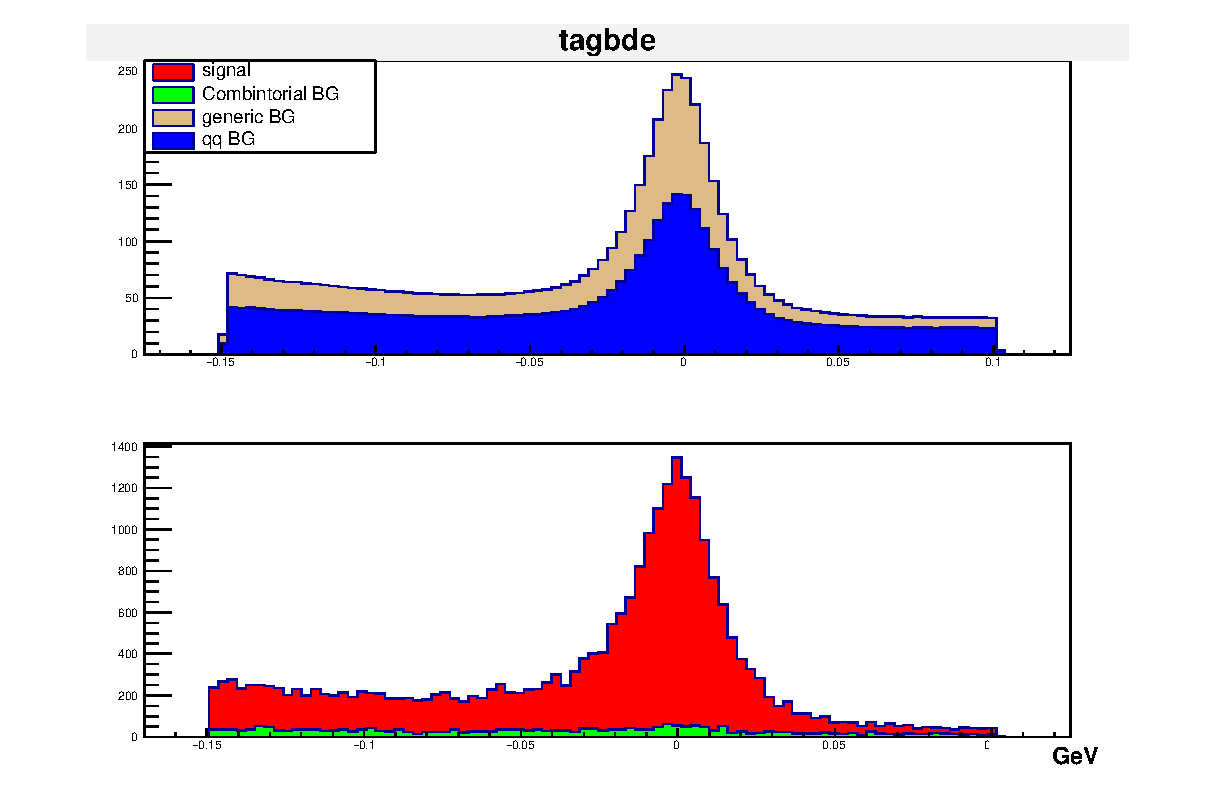
\includegraphics[width=0.45\textwidth]{eventselection_figure/tagbde_1025_1_kspi.eps}
		\label{kspide}
	}
    \subfigure[$K^{*0}$ mode.]{
		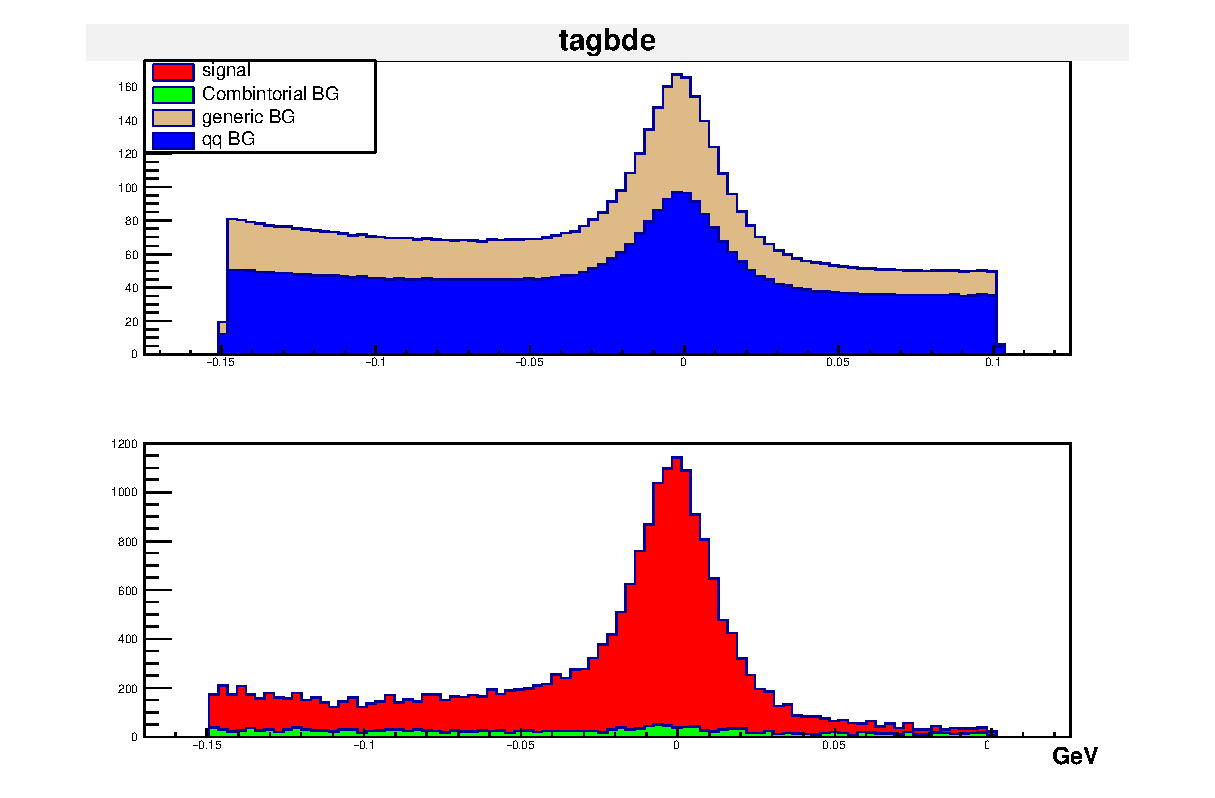
\includegraphics[width=0.45\textwidth]{eventselection_figure/tagbde_1025_1_b0kst.eps}
		\label{k0de}
	}
    \subfigure[$K_s$ mode.]{
		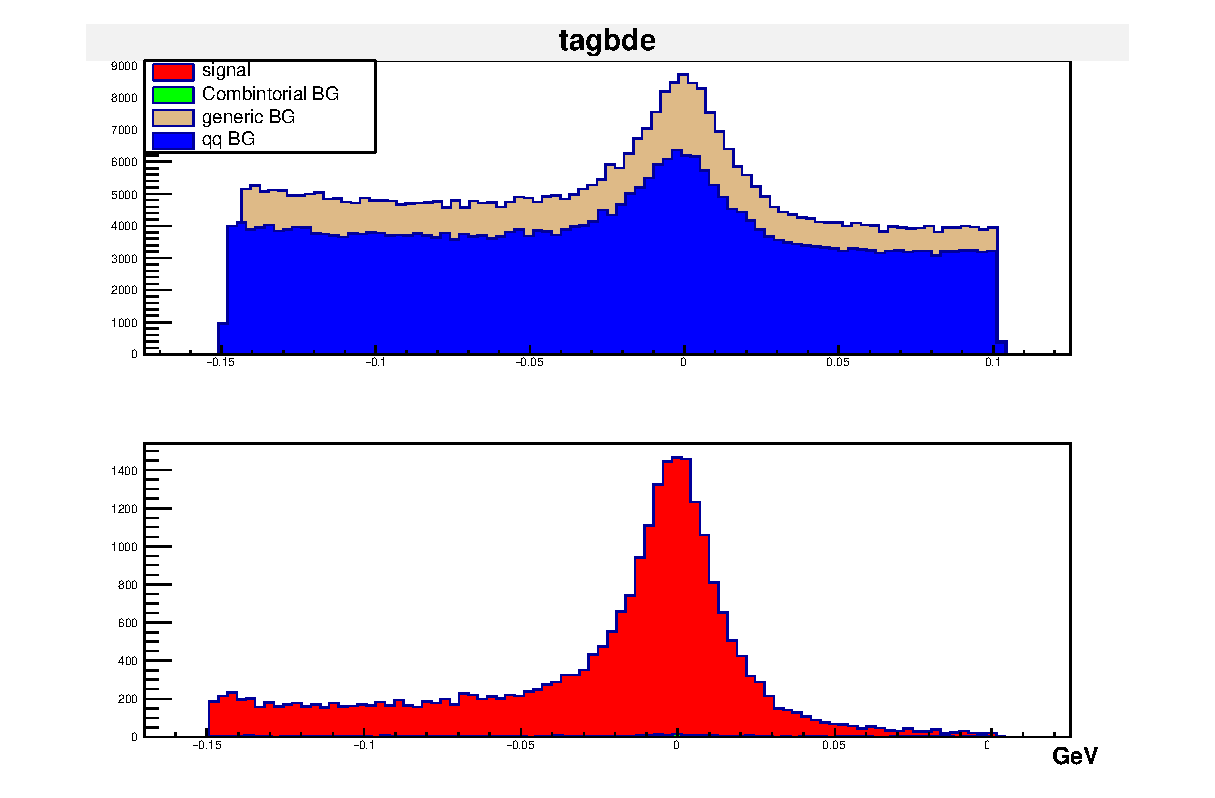
\includegraphics[width=0.45\textwidth]{eventselection_figure/tagbde_1025_1_b0ksh.eps}
		\label{ksde}
	}
	\caption{Tad-side $\Delta E$ distribution for each mode. Red represent signal, green represent the combinatorial background,  brown represent the generic background and blue represent continuum background.}
    	\label{fig:tagbde}	


    \end{figure}


    \begin{figure}[ht]
	\centering
	\subfigure[$K^{\pm}$ mode.]{
		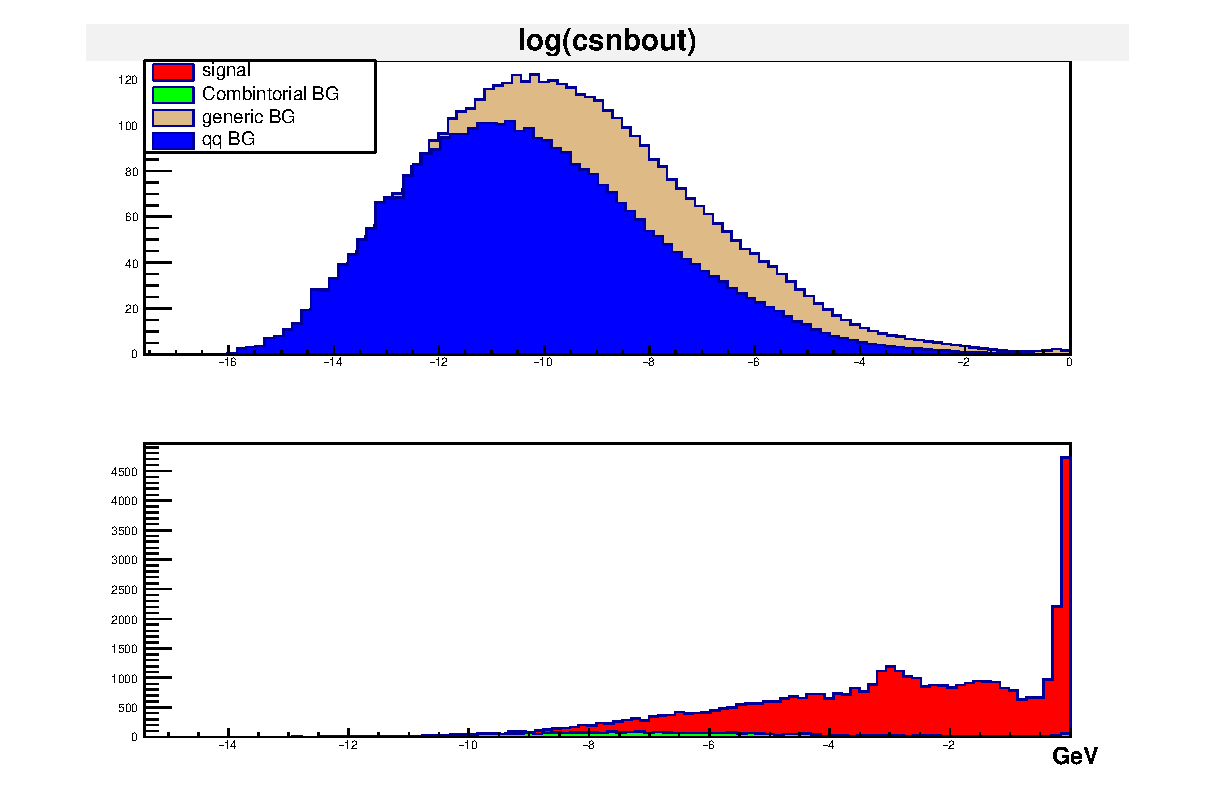
\includegraphics[width=0.45\textwidth]{eventselection_figure/log_csnbout__1025_1.eps}
		\label{knbout}
	}
	\subfigure[$K^{*\pm} \rightarrow K^\pm \pi^0$ mode.]{
		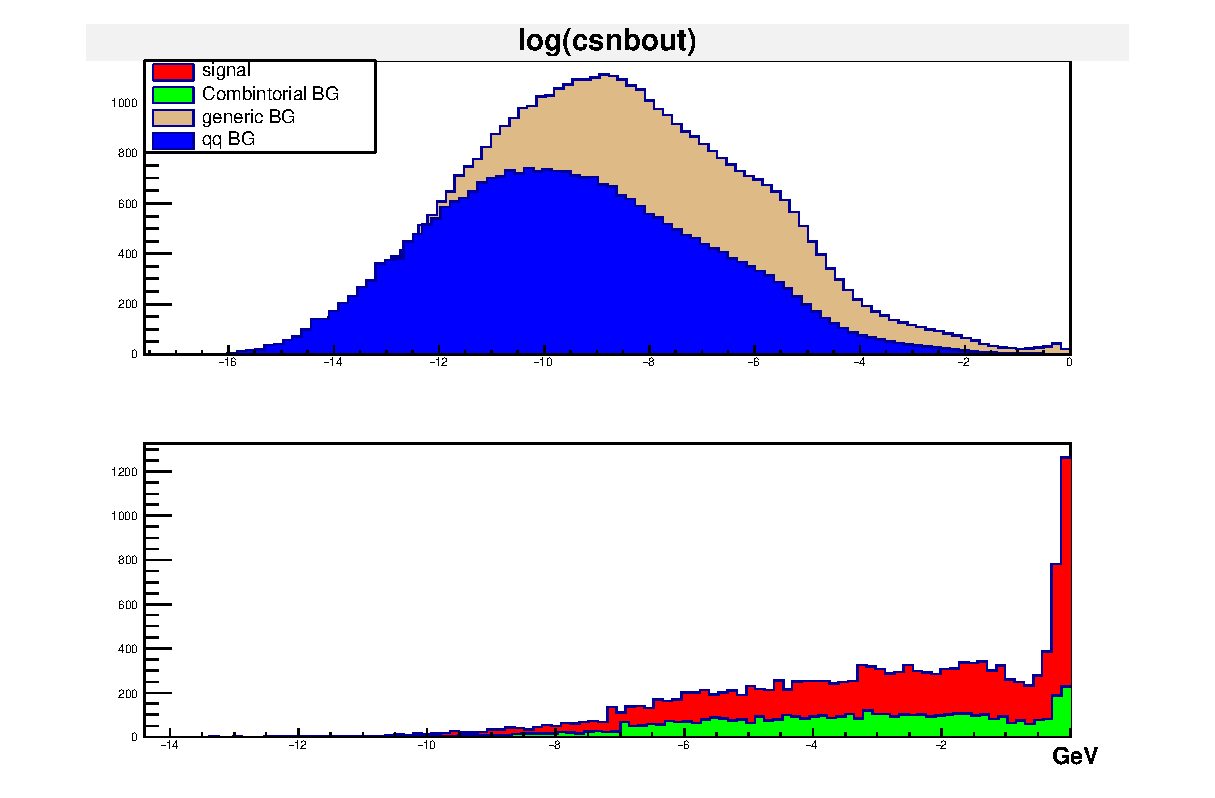
\includegraphics[width=0.45\textwidth]{eventselection_figure/log_csnbout__1025_1_kpi0.eps}
		\label{kpi0nbout}
	}
	\subfigure[$K^{*\pm} \rightarrow K_s \pi^\pm$ mode.]{
		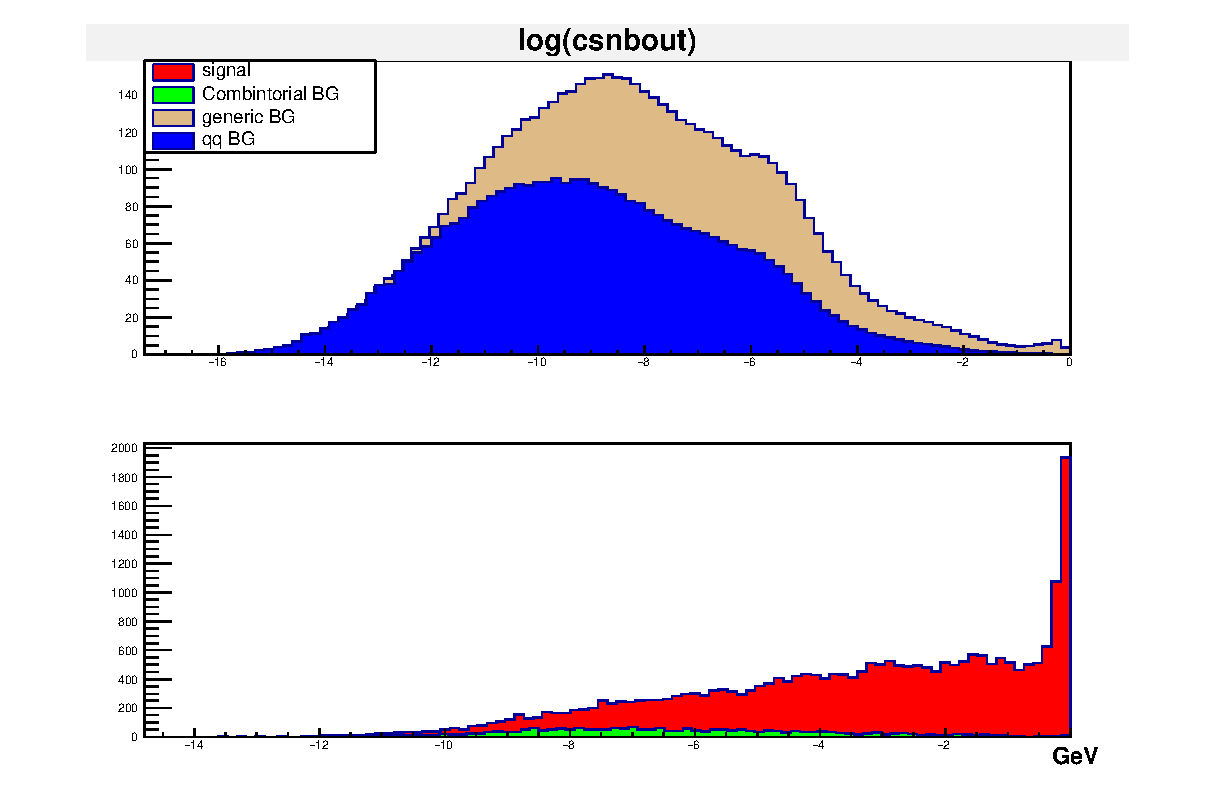
\includegraphics[width=0.45\textwidth]{eventselection_figure/log_csnbout__1025_1_kspi.eps}
		\label{kspinbout}
	}
    \subfigure[$K^{*0}$ mode.]{
		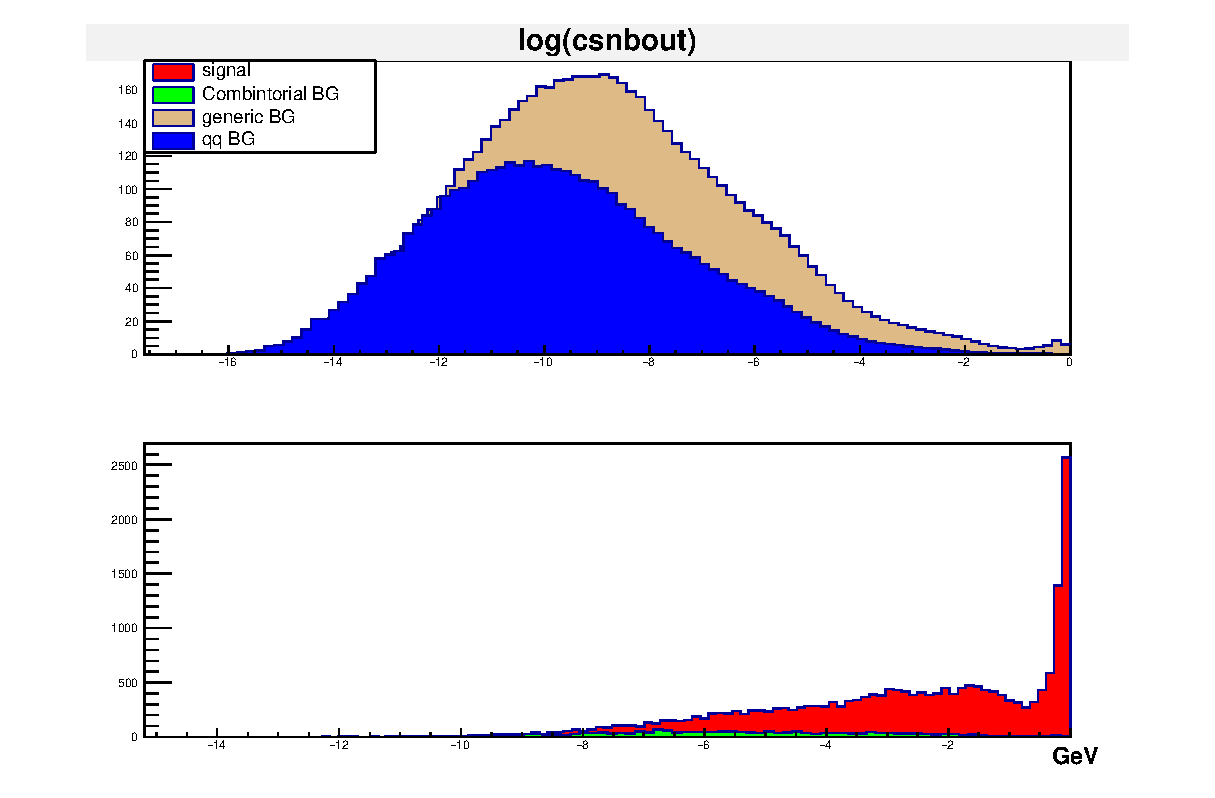
\includegraphics[width=0.45\textwidth]{eventselection_figure/log_csnbout__1025_1_b0kst.eps}
		\label{k0nbout}
	}
    \subfigure[$K_s$ mode.]{
		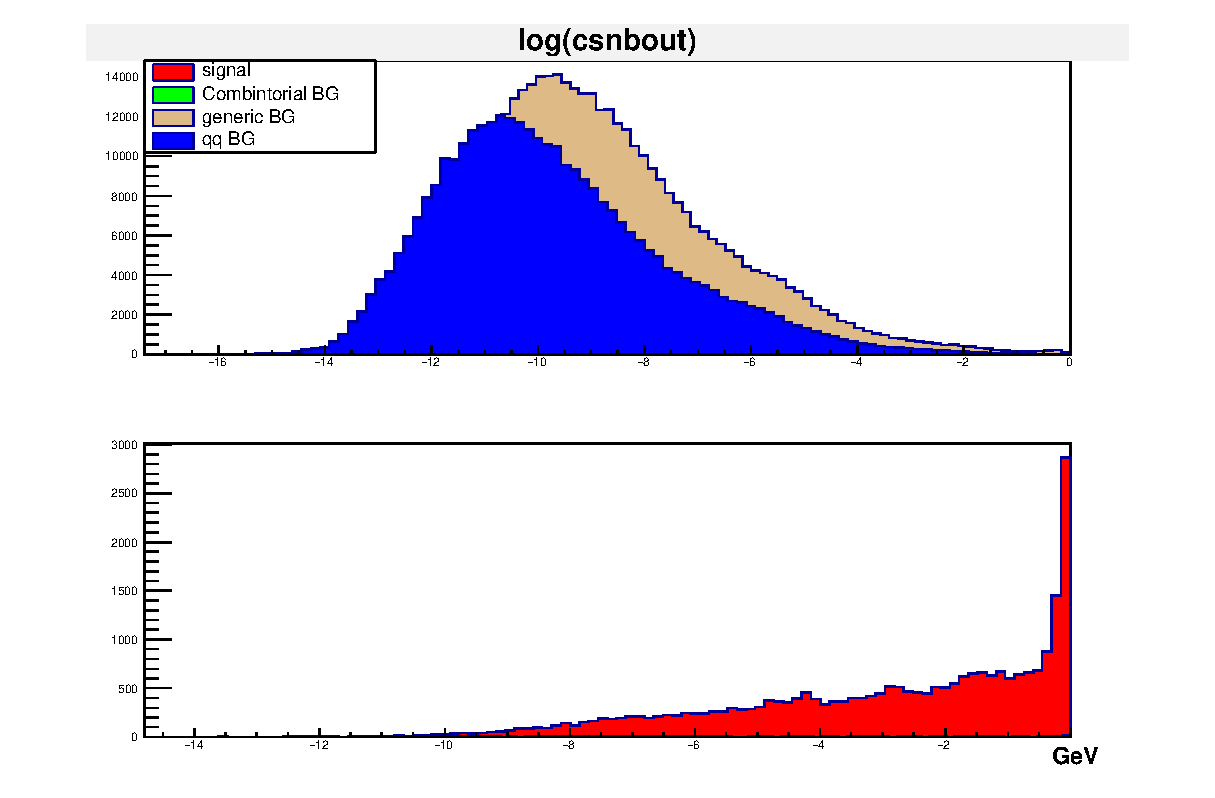
\includegraphics[width=0.45\textwidth]{eventselection_figure/log_csnbout__1025_1_b0ksh.eps}
		\label{ksnbout}
	}
	\caption{Tad-side NB output with continuum suppression $O_{tag}$ distribution for each mode. Red represent signal, green represent the combinatorial background,  brown represent the generic background and blue represent continuum background.}
    	\label{fig:nbout}	
\end{figure}

    \begin{figure}[ht]
	\centering
	\subfigure[$K^{\pm}$ mode.]{
		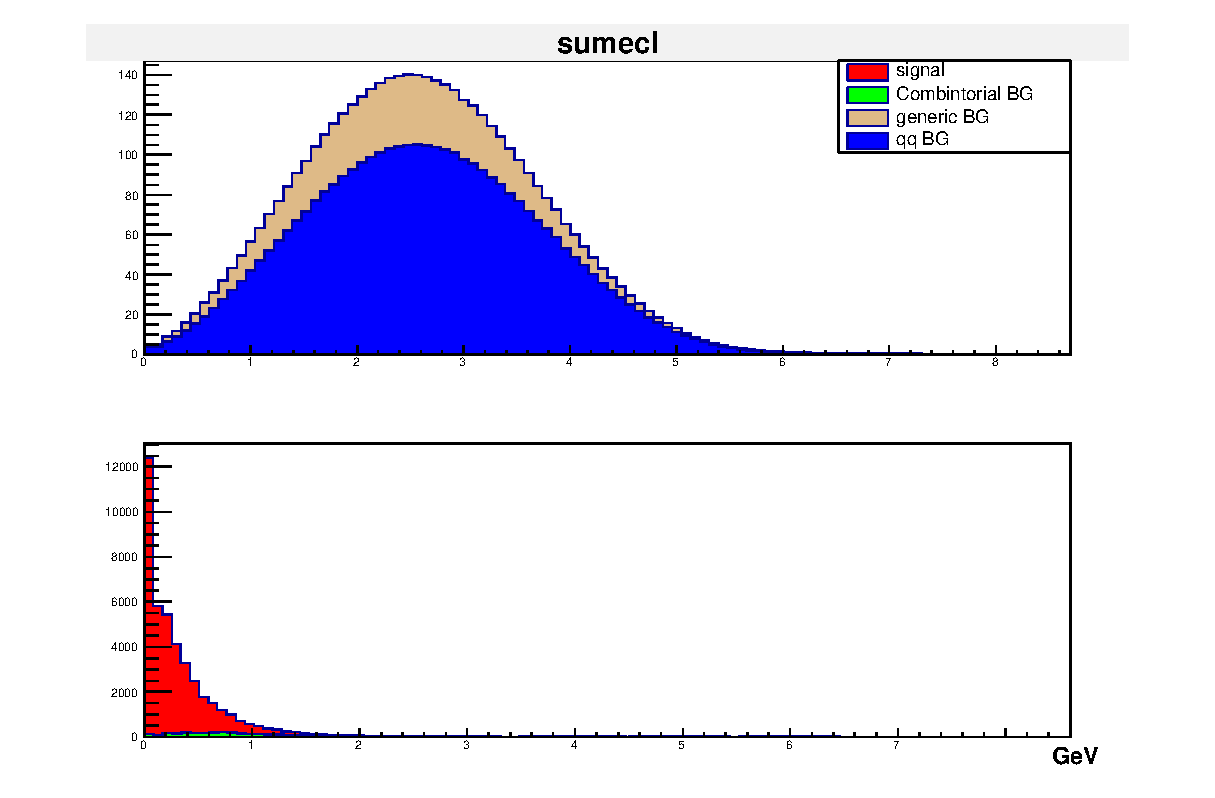
\includegraphics[width=0.45\textwidth]{eventselection_figure/sumecl_1025_1.eps}
		\label{ksumecl}
	}
	\subfigure[$K^{*\pm} \rightarrow K^\pm \pi^0$ mode.]{
		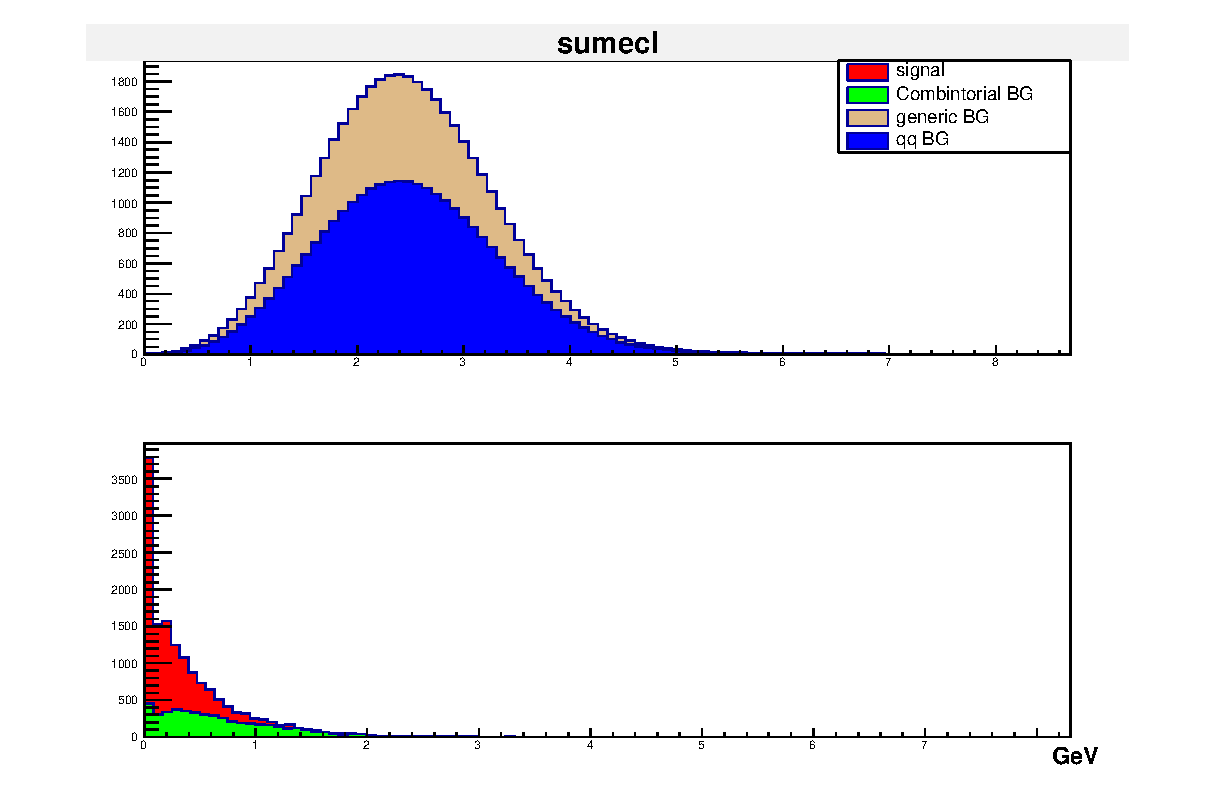
\includegraphics[width=0.45\textwidth]{eventselection_figure/sumecl_1025_1_kpi0.eps}
		\label{kpi0sumecl}
	}
	\subfigure[$K^{*\pm} \rightarrow K_s \pi^\pm$ mode.]{
		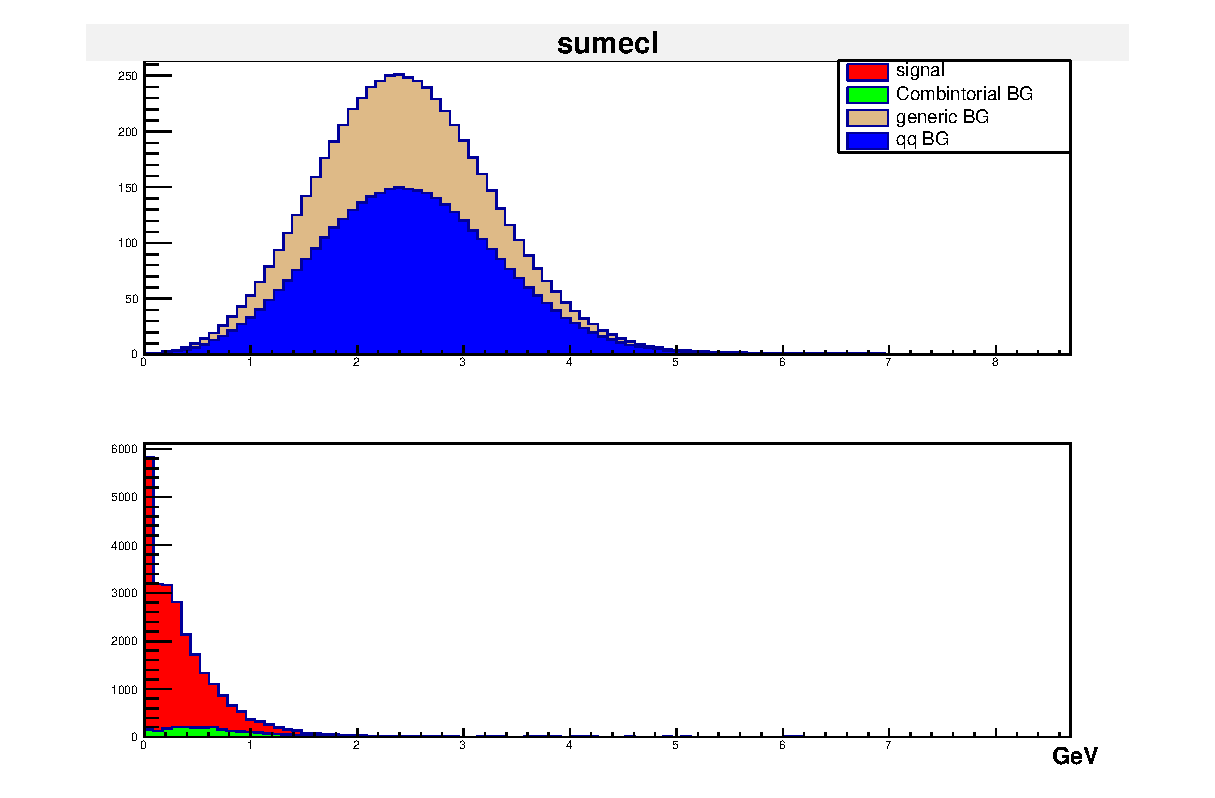
\includegraphics[width=0.45\textwidth]{eventselection_figure/sumecl_1025_1_kspi.eps}
		\label{kspisumecl}
	}
    \subfigure[$K^{*0}$ mode.]{
		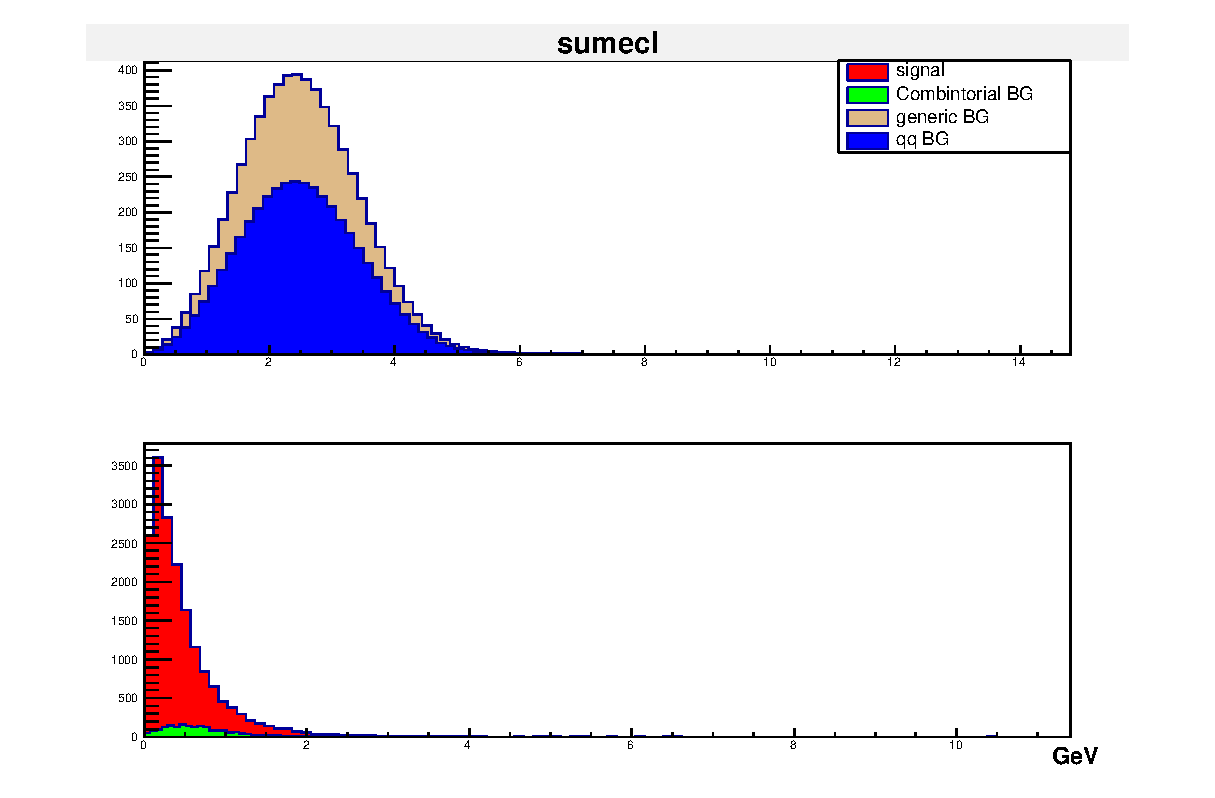
\includegraphics[width=0.45\textwidth]{eventselection_figure/sumecl_1025_1_b0kst.eps}
		\label{k0sumecl}
	}
    \subfigure[$K_s$ mode.]{
		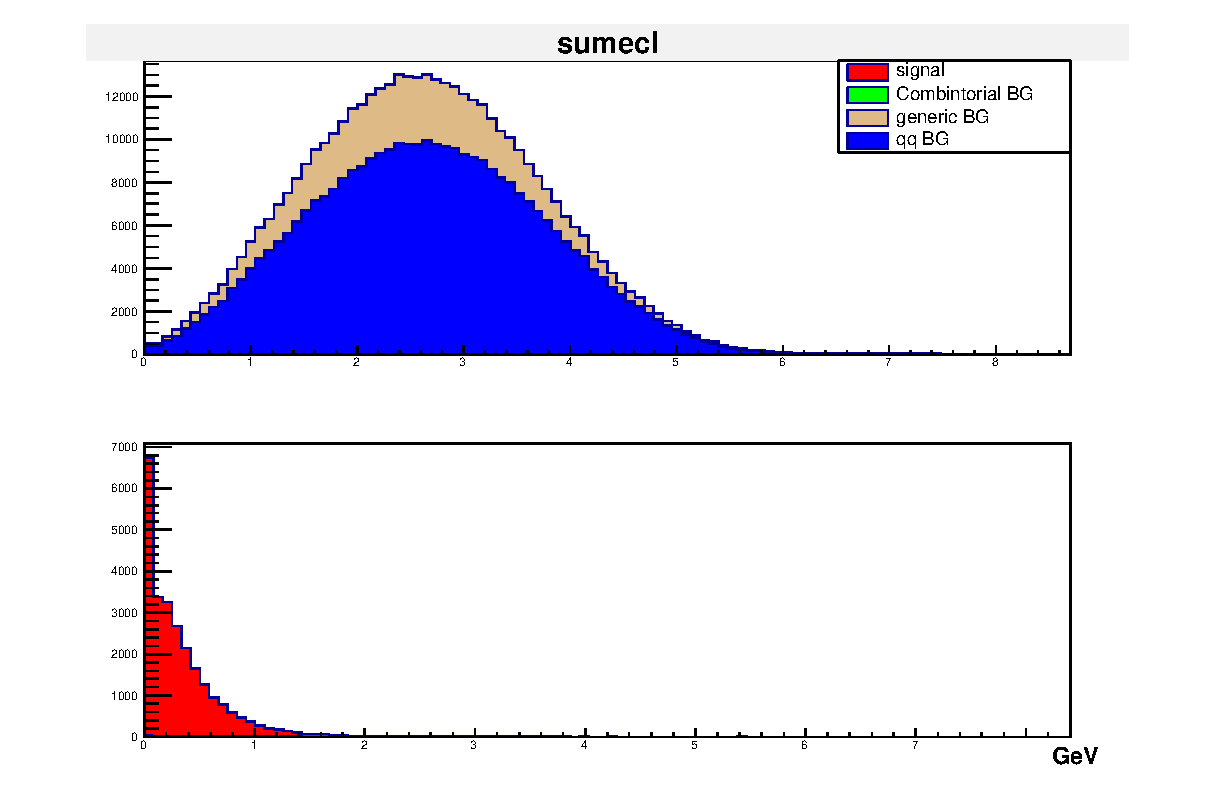
\includegraphics[width=0.45\textwidth]{eventselection_figure/sumecl_1025_1_b0ksh.eps}
		\label{kssumecl}
	}
\caption{Remaining energy $E_{ECL}$ distribution for each mode. Red represent signal, green represent the combinatorial background,  brown represent the generic background and blue represent continuum background.}
\label{fig:sumecl}	
\end{figure}
%%%%%%%%%%%%%%%%%%%%%%%%%%%%%%%%%%%%%%%%%%%%%%%%%%%%%%%%%%%%%%%%%%%%%%%%%%%%%%%%%%%%
\begin{table}[ht]
\small
\begin{center}
\begin{tabular}{ |p{2.2cm}||p{3.6cm}||p{2.8cm}||p{2.1cm}||p{1.3cm}|| }
\hline
 Cut					& Sig Efficiency$\times10^{-3}$  & generic BG$\times10^{4}$&qq BG$\times10^{4}$& com BG \\
\hline
\hline
  Fullrecon \& Track 		& $6.05\pm 0.03 $ 	& $ 10300\pm 1.01 $ 	&  $ 22900\pm1.51$	&7.30\%  \\ % &   $1.03 \times 10^{8}$&   $2.33 \times 10^{8}$ \\
 \hline
 $B_{\rm{tag}}M_{\rm{bc}} $  		& $5.96\pm 0.03$ 	& $ 6510\pm 0.81 $      & $ 14400\pm1.2 $	&4.50\%\\ %&   $3.77 \times 10^{7}$&   $8.93 \times 10^{7}$ \\
 \hline
 $ | B{\rm{tag}}\Delta E | $  		& $4.00 \pm 0.02$	& $ 3710\pm 0.61 $	& $  7430\pm0.86 $ 	&3.39\%\\ % &  $2.19 \times 10^{7}$ &   $4.70 \times 10^{7}$ \\
 \hline
 $E_{\rm{ecl}} $			& $3.96\pm 0.02$	& $ 969\pm 0.31$	& $ 1900\pm0.44 $ 	&2.88\%\\ % &  $5.86 \times 10^{6}$&   $1.22 \times 10^{7}$\\
 \hline
 n\_ track==0 				& $3.50\pm 0.02$	&$10.91\pm 0.03$	& $28.59\pm0.053$	&1.39\%\\ % &   $73524$&   $224138$ \\
 \hline		
$log(\rm{o_{tag}})$ 			& $3.45\pm 0.02$	&$6.35	\pm 0.03$	& $6.17 \pm0.024$	&1.12\% \\ %&   $1692$ &   $2555$\\
 \hline
\end{tabular}
\caption{$K^\pm$ mode: The efficiency drop and background level for each basic selection. The percentage of com BG means the fraction of the combinatorial background in signal MC. } \label{t:efficiency_k}

\end{center}
\end{table}

\begin{table}[ht]
 \small
\begin{center}
\begin{tabular}{ |p{2.2cm}||p{3.6cm}||p{2.8cm}||p{2.1cm}||p{1.3cm}|| }
 \hline
 Cut						& Sig Efficiency$\times10^{-3}$  & generic BG$\times10^{4}$&qq BG$\times10^{4}$& com BG \\
\hline
\hline
  Fullrecon \& Track 			& $1.37 \pm 0.01$ 	& $ 4496\pm0.67 $ 	&  $ 4849 \pm0.7$& 40.7\% \\ % &   $1.03 \times 10^{8}$&   $2.33 \times 10^{8}$ \\
 \hline
  $ M_{K^{* \pm}}  $  				& $1.29\pm 0.01$  	& $ 1560\pm0.40 $	& $ 370\pm0.19 $ & 32.5\%\\ % &   $5.95 \times 10^{7}$  &   $1.42 \times 10^{8}$\\
  \hline
 $B_{\rm{tag}}M_{\rm{bc}} $  			& $1.27\pm 0.01$ 	& $ 974\pm0.31$		& $ 229\pm0.15 $ &31.8\%\\ %&   $3.77 \times 10^{7}$&   $8.93 \times 10^{7}$ \\
 \hline
 $ | B{\rm{tag}}\Delta E | $  			& $1.00\pm 0.01$	& $ 586 \pm0.24$	& $ 132\pm0.12 $ &33.2\%\\ % &  $2.19 \times 10^{7}$ &   $4.70 \times 10^{7}$ \\
 \hline
 $E_{\rm{ecl}} $				& $0.999\pm 0.01 $	& $ 173\pm0.13$		& $ 38\pm0.06 $ &32.9\%\\ % &  $5.86 \times 10^{6}$&   $1.22 \times 10^{7}$\\
 \hline
 n\_ track==0 					& $0.977\pm 0.01 $	& $0.34\pm0.006$ 	& $2.3\pm0.02$  &32.5\%\\ % &   $73524$&   $224138$ \\
 \hline		
$log(\rm{o_{tag}})$ 				& $0.957\pm 0.01 $	& $0.18\pm0.004$	& $0.54\pm0.007$ &32.7\% \\ %&   $1692$ &   $2555$\\
 \hline
\end{tabular}
\caption{$K^{*\pm} \rightarrow K^+ \pi^0$ mode: The efficiency drop and background level for each basic selection. The percentage of com BG means the fraction of the combinatorial background in signal MC. } \label{t:efficiency_kpi0}
\end{center}
\end{table}
%%%%%%%%%%%%%%%%%%%%%%%%%%%%%%%%%%%%%%%%%%%%%%%%%%%%%%%%%%%%%%%%%%%%%%%%%%%%%%%%%%%%%%
\begin{table}[ht]
 \small
\begin{center}
\begin{tabular}{ |p{2.2cm}||p{3.6cm}||p{2.8cm}||p{2.1cm}||p{1.3cm}|| }
 \hline
 Cut& Sig Efficiency$\times10^{-3}$  & generic BG$\times10^{4}$&qq BG$\times10^{4}$& com BG \\
\hline
\hline
  Fullrecon \& Track 			& $2.981 \pm 0.02$ 	& $ 278 \pm 0.17$ 	&  $ 432 \pm 0.21$& 9.8\% \\ % &   $1.03 \times 10^{8}$&   $2.33 \times 10^{8}$ \\
 \hline
  $  M_{K^{* \pm}}  $  				& $2.979 \pm 0.02$  	& $ 228 \pm 0.15$	& $ 370 \pm 0.19$ & 9.7\%\\ % &   $5.95 \times 10^{7}$  &   $1.42 \times 10^{8}$\\
  \hline
 $B_{\rm{tag}}M_{\rm{bc}} $  			& $2.94 \pm 0.02$ 	& $ 142 \pm 0.11$	 & $ 229 \pm 0.15$ &6.5\%\\ %&   $3.77 \times 10^{7}$&   $8.93 \times 10^{7}$ \\
 \hline
 $ | B{\rm{tag}}\Delta E | $  			& $2.09 \pm 0.02$	& $88.32\pm 0.09$	& $132\pm 0.12$ &4.3\%\\ % &  $2.19 \times 10^{7}$ &   $4.70 \times 10^{7}$ \\
 \hline
 $E_{\rm{ecl}} $				& $2.07 \pm 0.02$	& $26.68\pm 0.05$	& $37.5\pm 0.06$ &4.2\%\\ % &  $5.86 \times 10^{6}$&   $1.22 \times 10^{7}$\\
 \hline
 n\_ track==0 					& $1.98 \pm 0.02$	&$0.879\pm 0.01 $	& $2.35\pm 0.015$  &3.3\%\\ % &   $73524$&   $224138$ \\
 \hline		
$log(\rm{o_{tag}})$ 				& $1.91 \pm 0.02$	&$0.490\pm 0.007$ 	& $0.54\pm 0.007$ &2.6\% \\ %&   $1692$ &   $2555$\\
 \hline
\end{tabular}
\caption{$K^{*\pm} \rightarrow K_s \pi^\pm$ mode: The efficiency drop and background level for each basic selection. The percentage of com BG means the fraction of the combinatorial background in signal MC. } \label{t:efficiency_kspi}
\end{center}
\end{table}

\begin{table}[ht]
 \small
\begin{center}
\begin{tabular}{ |p{2.2cm}||p{3.6cm}||p{2.8cm}||p{2.1cm}||p{1.3cm}|| }
 \hline
 Cut& Sig Efficiency$\times10^{-3}$  & generic BG$\times10^{4}$&qq BG$\times10^{4}$& com BG \\
\hline
\hline
  Fullrecon \& Track\&$M_{K*0} $	& $(2.47\pm 0.02)$ 	&$1558\pm  0.395$&$2771\pm 0.526$&9.88\% \\ % &   $1.03 \times 10^{8}$&   $2.33 \times 10^{8}$ \\
 \hline
 $B_{\rm{tag}}M_{\rm{bc}}$  			& $(2.44\pm 0.02)$ 	&$972 \pm 0.312$&$1716 \pm 0.414$&6.59\%\\ %&   $3.77 \times 10^{7}$&   $8.93 \times 10^{7}$ \\
 \hline
 $ | B{\rm{tag}}\Delta E |$  			& $(1.79\pm 0.02)$	&$585 \pm 0.242$&$953 \pm0.309$	&4.00\%\\ % &  $2.19 \times 10^{7}$ &   $4.70 \times 10^{7}$ \\
 \hline
 $E_{\rm{ecl}}$					& $(1.78\pm 0.02$	&$173  \pm 0.132$&$270\pm0.164$	&3.94\%\\ % &  $5.86 \times 10^{6}$&   $1.22 \times 10^{7}$\\
 \hline
 n\_ track					& $(1.73 \pm 0.02)$	&$13.3\pm 0.04$	&$22.9\pm0.048$	&0.79\%\\ % &   $73524$&   $224138$ \\
 \hline		
$log(\rm{o_{tag}})$ 				& $(1.70 \pm0.01)$	&$7.64\pm0.03$	&$4.98\pm0.022$	&0.72\% \\ %&   $1692$ &   $2555$\\
 \hline
\end{tabular}
\caption{$K^{*0}$ mode: The efficiency drop and background level for each basic selection. The percentage of com BG means the fraction of the combintorial background in signal MC. } \label{t:efficiency_k0}
\end{center}
\end{table}
%%%%%%%%%%%%%%%%%%%%%%%%%%%%%%%%%%%%%%%%%%%%%%%%%%%%%%%%%%%%%%%%%%
\begin{table}[ht]
 \small
\begin{center}
\begin{tabular}{ |p{2.2cm}||p{3.6cm}||p{2.8cm}||p{2.1cm}||p{1.3cm}|| }
 \hline
 Cut& Sig Efficiency$\times10^{-3}$  & generic BG$\times10^{4}$&qq BG$\times10^{4}$& com BG \\
\hline
\hline
  Fullrecon \& Track\&$M_{K*0} $	& $(3.53\pm 0.02)$ &$601\pm 0.245$&$1210\pm 3479$	&2.77\% \\ % &   $1.03 \times 10^{8}$&   $2.33 \times 10^{8}$ \\
 \hline
 $B_{\rm{tag}}M_{\rm{bc}}$  		& $(3.49\pm 0.02)$ &$383 \pm 0.196$&$761 \pm 0.275$	&1.70\%\\ %&   $3.77 \times 10^{7}$&   $8.93 \times 10^{7}$ \\
 \hline
 $ | B{\rm{tag}}\Delta E |$  		& $(2.56\pm 0.02)$	&$223 \pm 0.149$&$401 \pm0.200$	&1.23\%\\ % &  $2.19 \times 10^{7}$ &   $4.70 \times 10^{7}$ \\
 \hline
 $E_{\rm{ecl}}$				& $(2.52 \pm 0.02$	&$57\pm0.076$&$97\pm0.099$	&1.19\%\\ % &  $5.86 \times 10^{6}$&   $1.22 \times 10^{7}$\\
 \hline
 n\_ track					& $(2.40 \pm 0.02)$	&$0.95\pm0.01$&$2.69\pm0.016$	&0.79\%\\ % &   $73524$&   $224138$ \\
 \hline		
$log(\rm{o_{tag}})$ 				& $(2.33\pm0.02)$	&$0.53\pm0.007$&$0.56\pm0.008$	&0.72\% \\ %&   $1692$ &   $2555$\\
 \hline
\end{tabular}
\caption{$K_s$ mode: The efficiency drop and background level for each basic selection. The percentage of com BG means the fraction of the combinatorial background in signal MC. } \label{t:efficiency_ks}\end{center}
\end{table}
%%%%%%%%%%%%%%%%%%%%%%%%%%%%%%%%%%%%%%%%%%%%%%%%%%%%%%%%%%%%%%%%%%%%%%%%%%%%%%%%%%%%%

\chapter{Model Independent Study}
\section{$S_b$ Distribution}
The $S_b$ is defined as $S_b \equiv q^2/m^2_B$, where $q^2$ is the squared magnitude of the four-momentum transferred from the B meson to the neutrino pairs, and the $m_B$ is the mass of B meson.  Instead make a requirement on signal side candidate($K^*$) momentum, which is highly correlated to the $S_b$, we keep the full $S_b$ spectrum and provide the model-independent study bin-by-bin on $S_b$ spectrum. In this study, we perform the bin-by-bin optimization and calculate the partial branching fractions($\Delta \mathcal{B}$) in intervals of $S_b = 0.1$. With the full spectrum study, we have the opportunity to probe the hint of new physics. The $S_b$ distribution shown in Fig. \ref{fig:sb}.
    \begin{figure}[ht]
	\centering
	\subfigure[$K^{\pm}$ mode.]{
		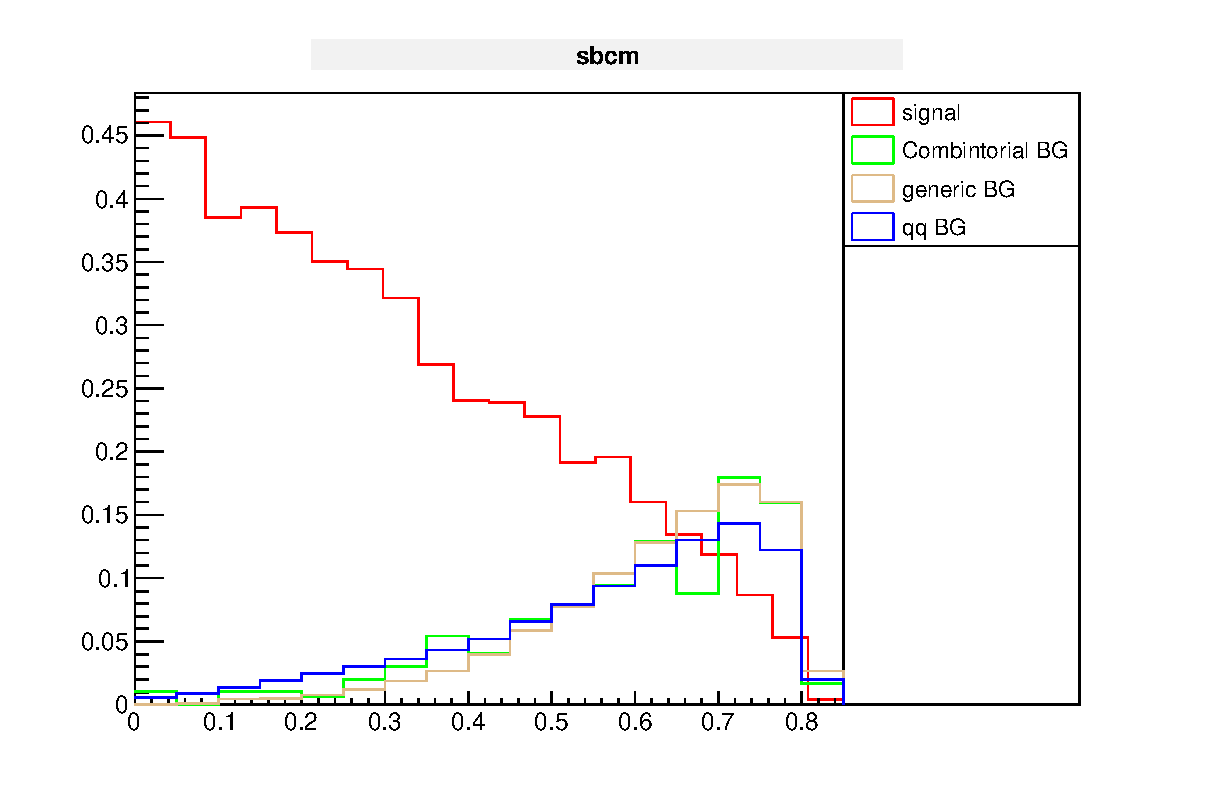
\includegraphics[width=0.45\textwidth]{bin_by_bin_study_figure/knunu/sbcm_1025_1.eps}
		\label{ksb}
	}
	\subfigure[$K^{*\pm} \rightarrow K^\pm \pi^0$ mode.]{
		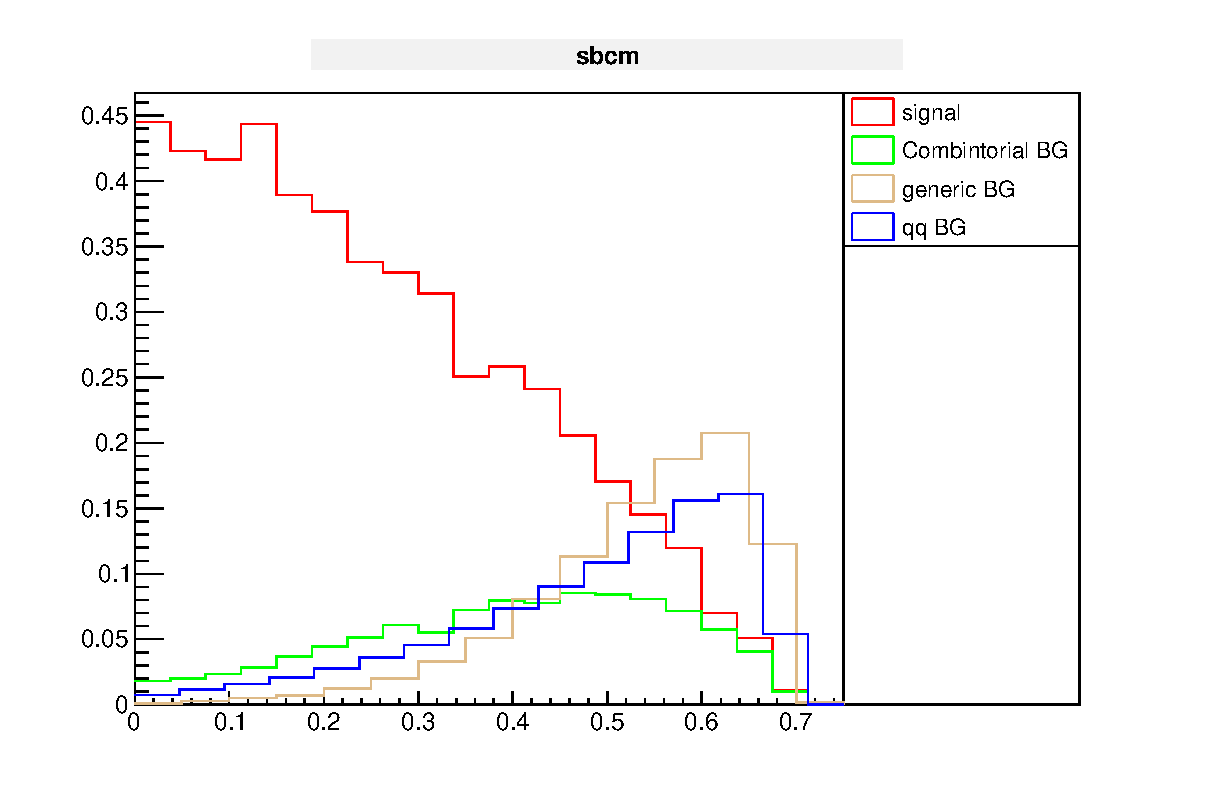
\includegraphics[width=0.45\textwidth]{bin_by_bin_study_figure/kstar1/sbcm_1025_kstar1.eps}
		\label{kpi0sb}
	}
	\subfigure[$K^{*\pm} \rightarrow K_s \pi^\pm$ mode.]{
		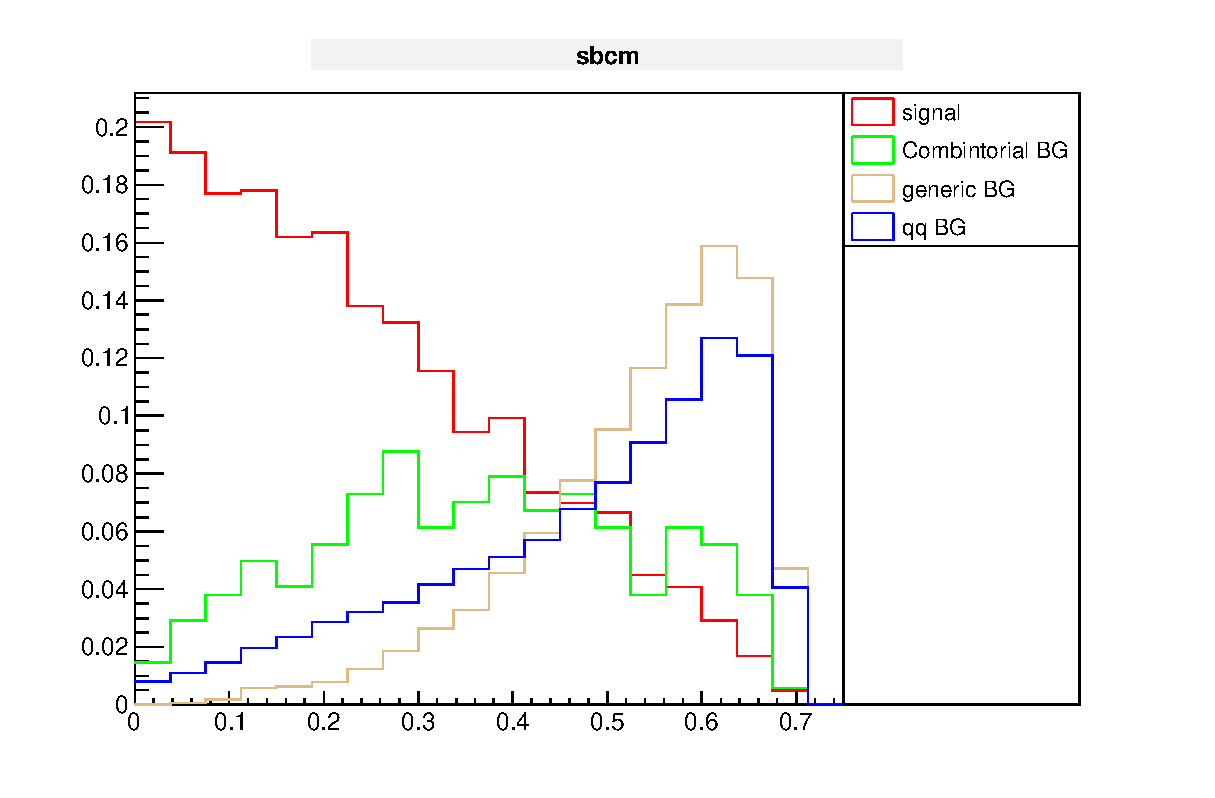
\includegraphics[width=0.45\textwidth]{bin_by_bin_study_figure/kstar2/sbcm_1025_112.eps}
		\label{kspisb}
	}
    \subfigure[$K^{*0}$ mode.]{
		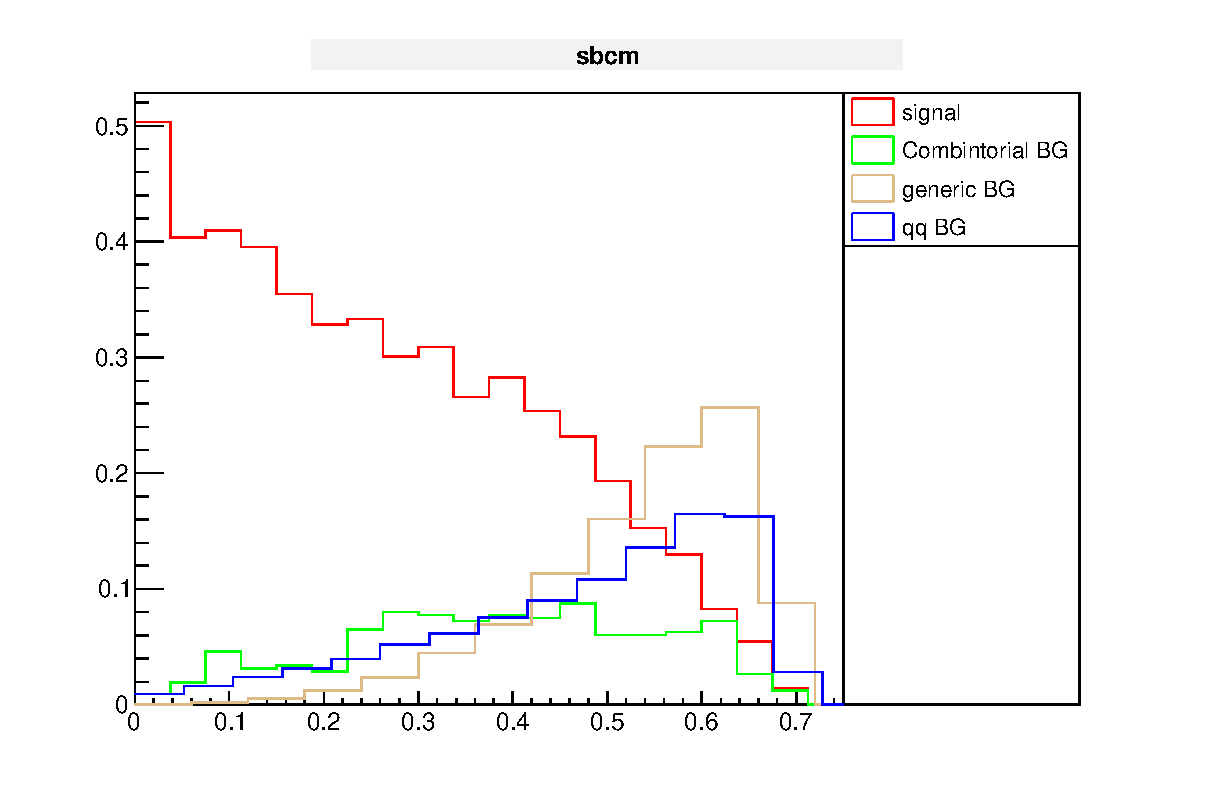
\includegraphics[width=0.45\textwidth]{bin_by_bin_study_figure/k0/sbcm_1025_1.eps}
		\label{k0sb}
	}
    \subfigure[$K_s$ mode.]{
		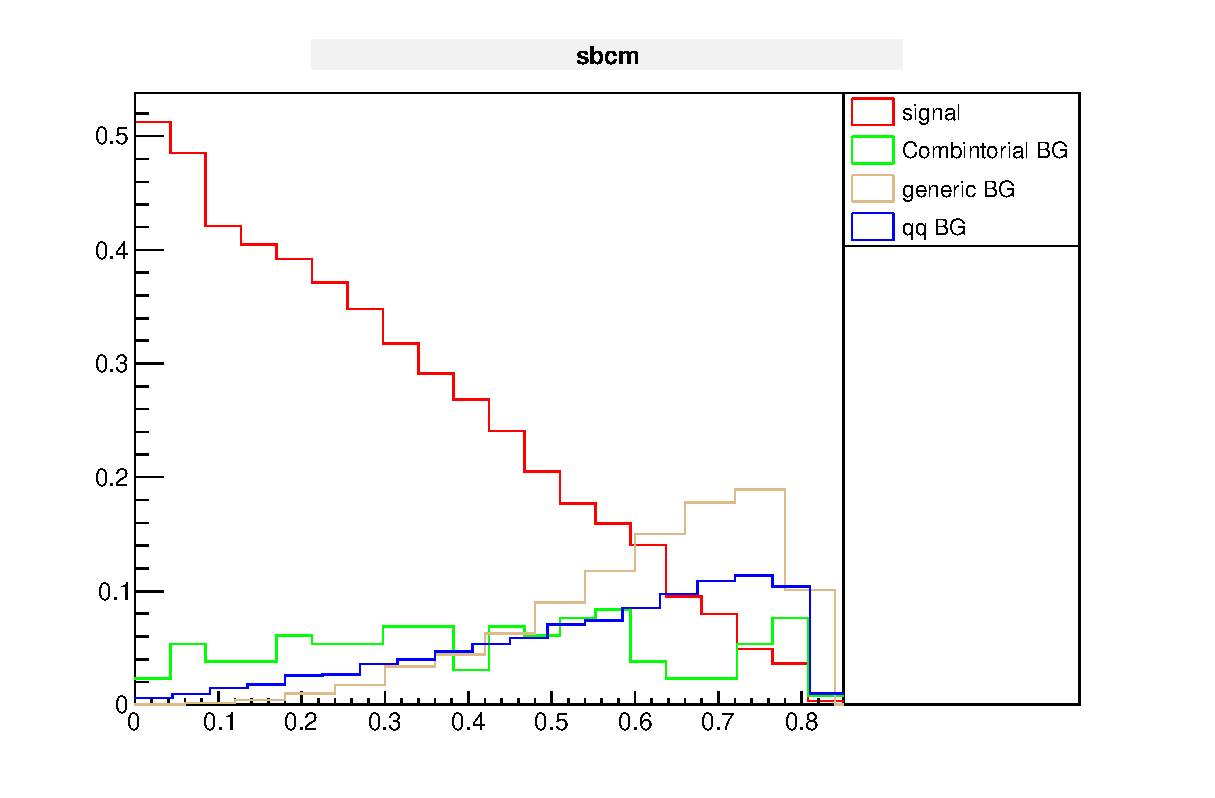
\includegraphics[width=0.45\textwidth]{bin_by_bin_study_figure/kshort/sbcm_1025_1.eps}
		\label{kssb}
	}
\caption{$S_b$ distribution for each mode. Red represent signal, green represent the combintorial background,  brown represent the generic background and blue represent continuum background.}
\label{fig:sb}	
\end{figure}
\section{Neural-Network training}
In order to do the further separation between signal and background bin-by-bin, the powerful neural-network based multivariate analysis package Neurobayes is used. In this study, we use two kind of variables to training twice. One kind of variables is aiming to reduce the generic background; the other kind is shape variable from KSFW(Kakuno san's super fox-wolfram)\cite{ref:Lee2003} \cite{ref:fox1978}, there are 23 variables in total. 
\subsection{Training result} 
For the first kind of training, which is aiming to get rid of the generic background, we use generic MC sample as the background candidate, signal correct reconstruct MC sample as the signal candidate.The variables we use in first kind of NB training are list in table \ref{t:nbvlike_variables}, some of the variables list in table are based on Sebastian Neubauer's study~\cite{ref:Neubauer2011}. For the second kind of training(KSFW variables), we use continuum MC sample as the background candidate, signal correct reconstruct MC sample as the signal candidate.The training result with the table \ref{t:nbvlike_variables} for each mode is shown in Fig. \ref{fig:nbvlike}, The training result with KSFW variables is shown in Fig. \ref{fig:nbksfw}.
\begin{table}[ht]
\small
\begin{center}
\begin{tabular}{ |p{3cm}||p{10cm}|  }
 \hline
 cut& Description \\
 \hline
 \hline
  $B{\rm{tag}}\Delta E$   &  $\Delta E$ of Btag candidate.    \\
 \hline
 $B{\rm{tag}}M_{\rm{bc}}$   &  $M_{\rm{bc}}$ of Btag candidate.   \\
 \hline
 n\_ trackAll    & Number of additional track without any cuts.(i.e. no restrict on dr, dz and $P_T$ )  \\
  \hline
 n\_ pi0all    & Number of additional $\pi_0$ without any cuts.(no restrict on momentum )  \\
 \hline
 cosMEcm & Angle between the missing momentum and the whole event in the center of mass rest frame.\\
 \hline
 cos$\theta_{\rm{k}}$& Angle between signal candidate and Beam-pipe in lab frame.\\
 \hline
B$\Delta$dz& The different between the mean $|dz|$ of tag-side B signal condidate.  \\
 \hline
B$\Delta$dzsign& The significance of B$\Delta$dz.\\
\hline
 SumeclInMMdDir& The total enery measured by the calorimeter in a small cone around the direction of the missing-momentum.\\
 \hline
  $log(\rm{o_{tag}})$ & continuous suppression $NB_{\rm{out}}$\\
 \hline
RatiotoOthertype & the ratio of this BTag candidates NBout and the best of the other type if there is one.\\
 \hline
RatiotoSecondBest & the ratio of this BTag candidates NBout to the second best of this type if there is one.\\
 \hline
  $K^*$ mass   &  The invariant mass of $K^{*}$ candidate.    \\
 \hline
  $K^*$ child1 mass   &  The invariant mass of $K^{*}$ candidate first child.    \\
 \hline
  $K^*$ child2 mass   &  The invariant mass of $K^{*}$ candidate second child.    \\
 \hline
  Ddecay   &  Decay hashes of the tag-side D meson    \\
 \hline
  Tag\_expid   &  Experiment ID    \\
 \hline
\end{tabular}

\caption{The variables use in first kind of NB training, which is aiming to reduce the generic background. } \label{t:nbvlike_variables}
\end{center}
\end{table}

   \begin{figure}[ht]
	\centering
	\subfigure[$K^{\pm}$ mode.]{
		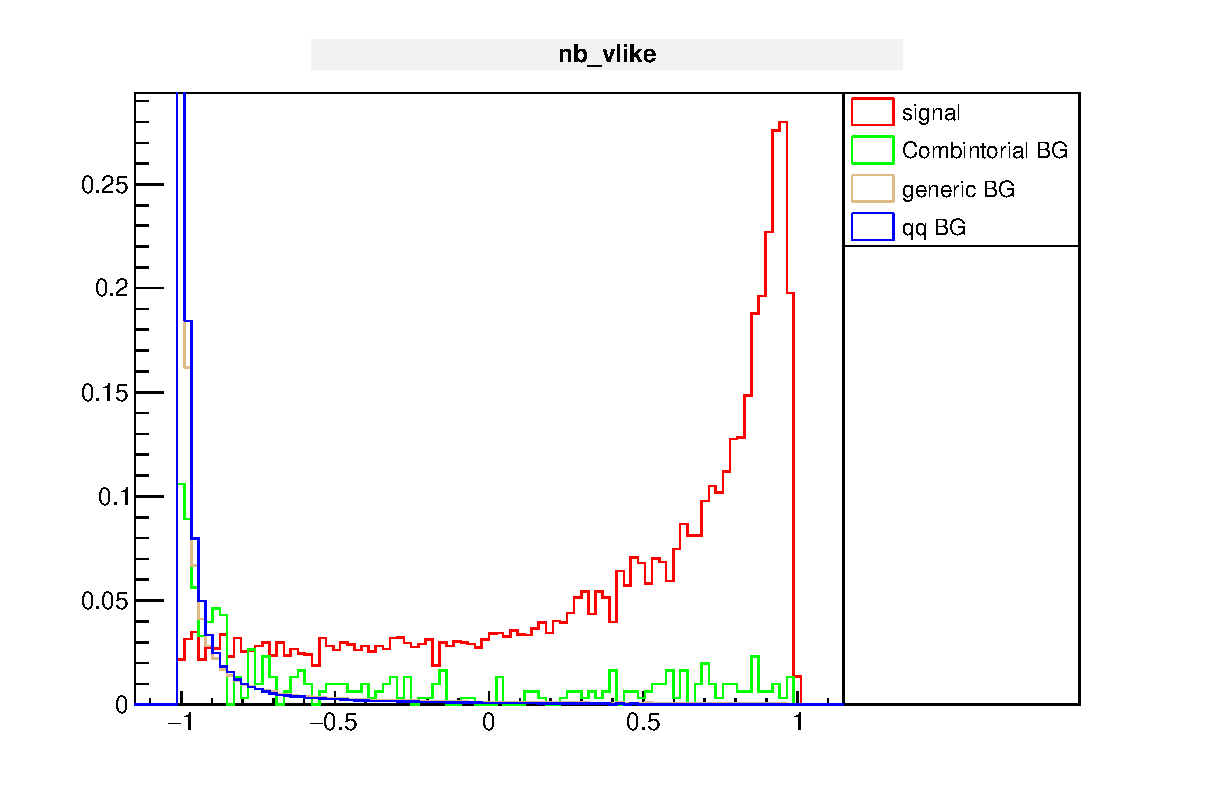
\includegraphics[width=0.45\textwidth]{bin_by_bin_study_figure/knunu/nb_vlike_1025_1.eps}
		\label{knbvlike}
	}
	\subfigure[$K^{*\pm} \rightarrow K^\pm \pi^0$ mode.]{
		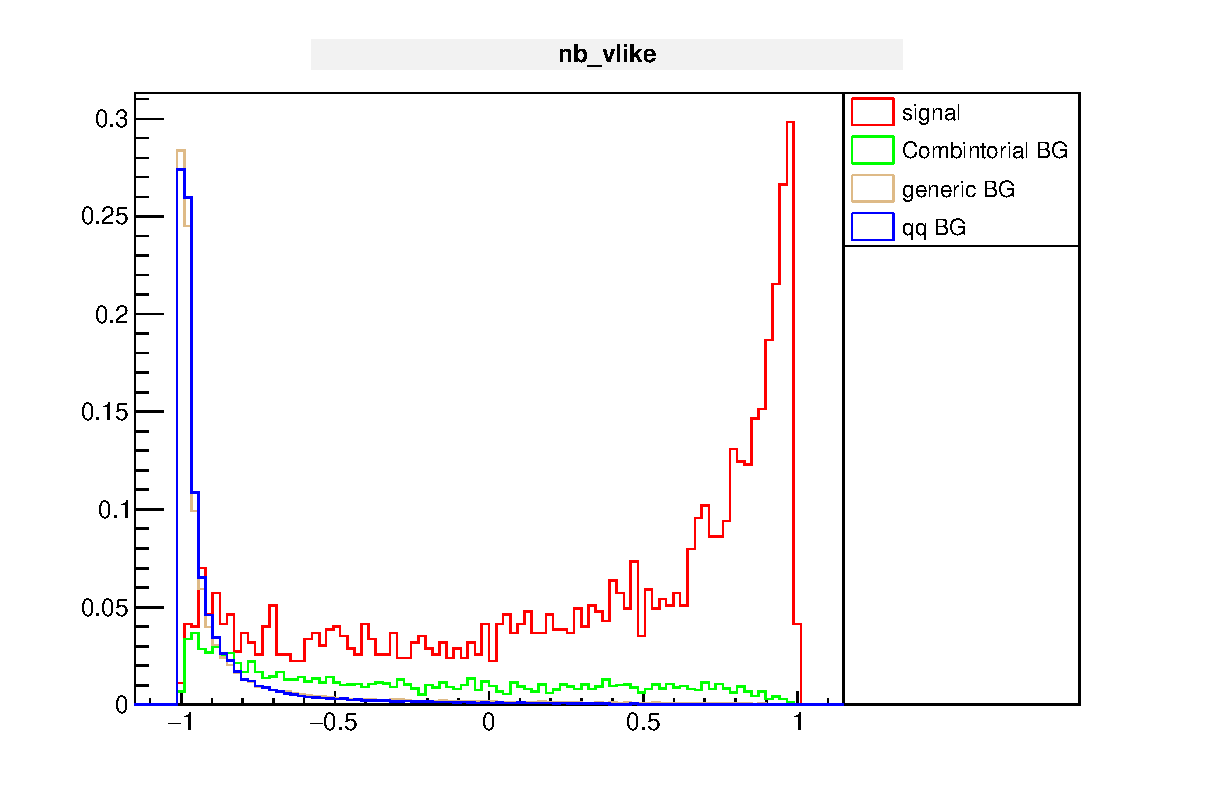
\includegraphics[width=0.45\textwidth]{bin_by_bin_study_figure/kstar1/nb_vlike_1025_kstar1.eps}
		\label{kpi0nbvlike}
	}
	\subfigure[$K^{*\pm} \rightarrow K_s \pi^\pm$ mode.]{
		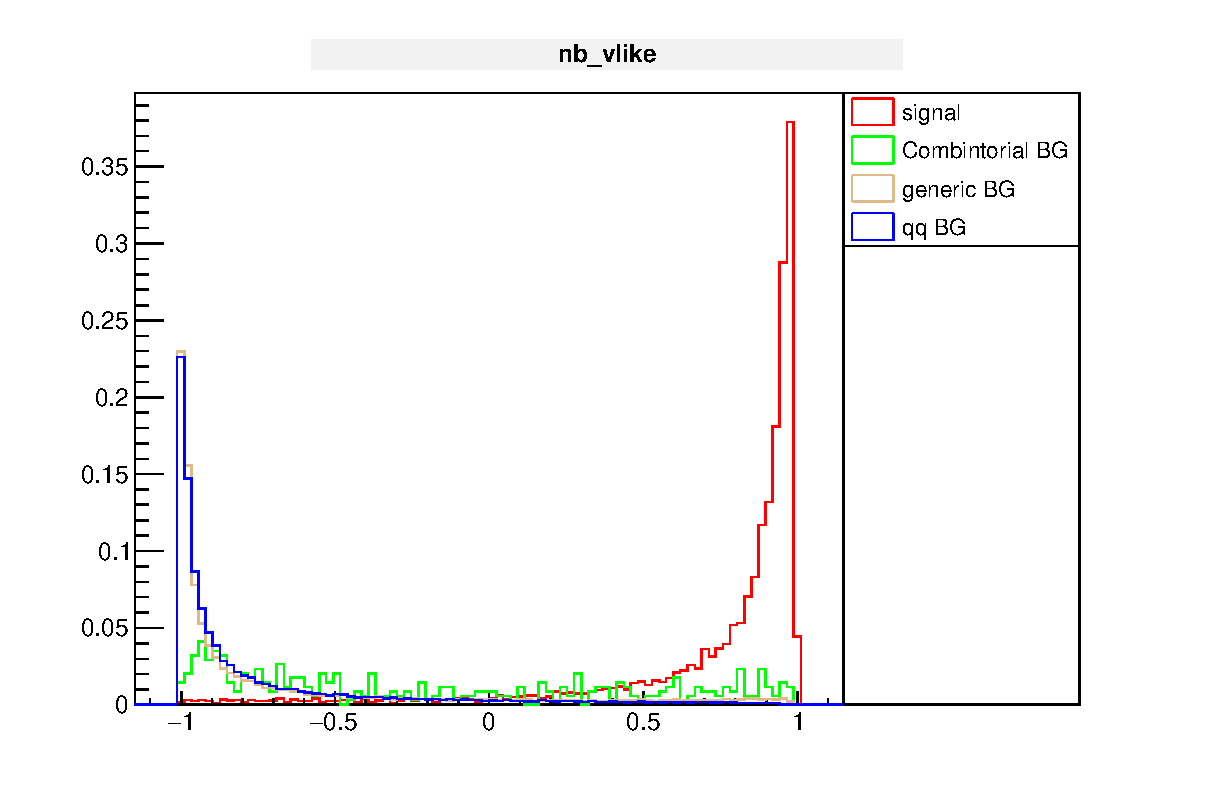
\includegraphics[width=0.45\textwidth]{bin_by_bin_study_figure/kstar2/nb_vlike_1025_112.eps}
		\label{kspinbvlike}
	}
    \subfigure[$K^{*0}$ mode.]{
		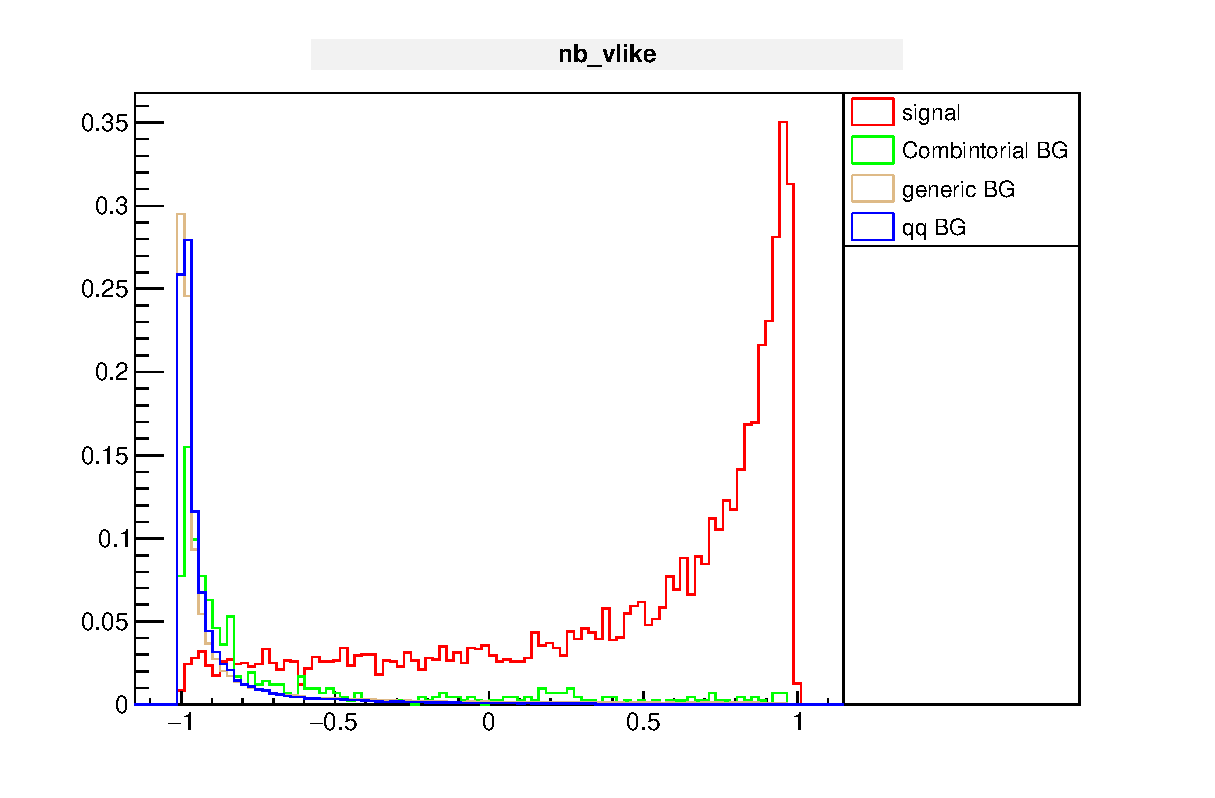
\includegraphics[width=0.45\textwidth]{bin_by_bin_study_figure/k0/nb_vlike_1025_1.eps}
		\label{k0nbvlike}
	}
    \subfigure[$K_s$ mode.]{
		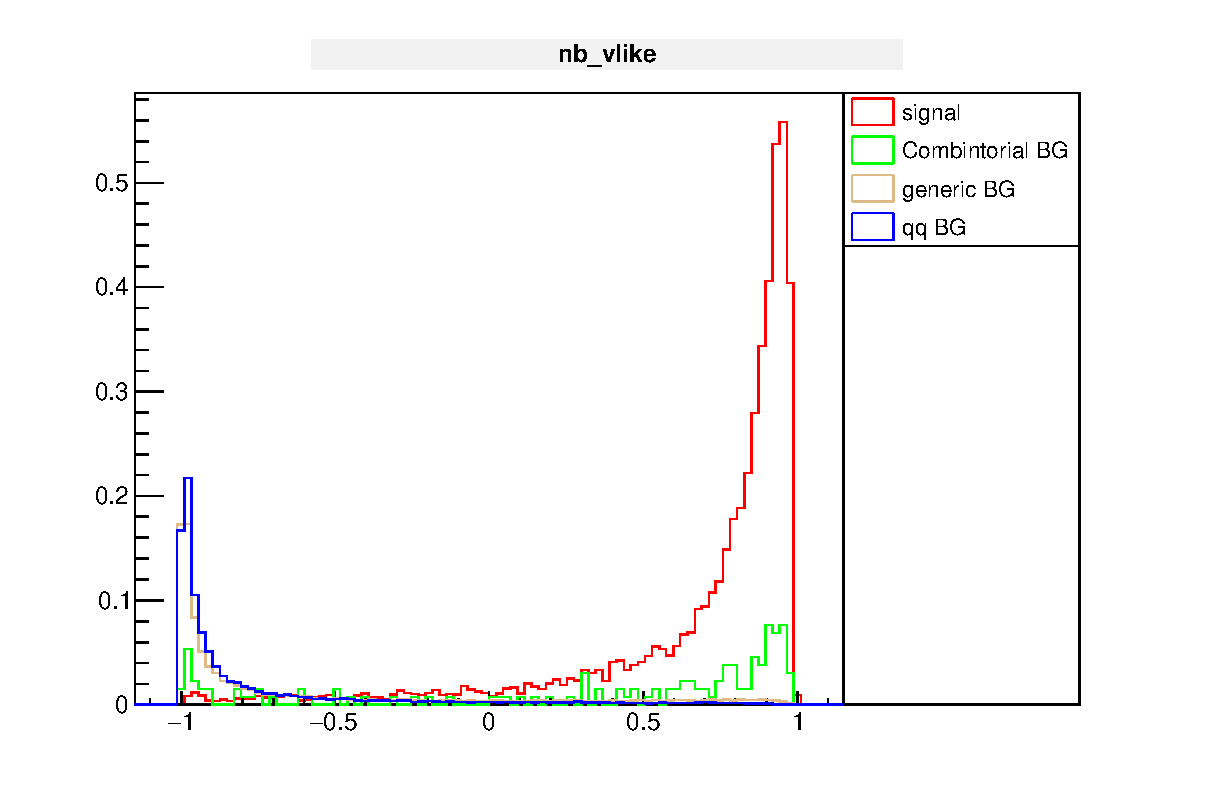
\includegraphics[width=0.45\textwidth]{bin_by_bin_study_figure/kshort/nb_vlike_1025_1.eps}
		\label{ksnbvlike}
	}
\caption{Neurobayes output with variables list in table \ref{t:nbvlike_variables} for each mode. Red line represent signal, green line represent the combinatorial background,  brown line represent the generic background and blue line represent continuum background.}
\label{fig:nbvlike}	
\end{figure}

   \begin{figure}[ht]
	\centering
	\subfigure[$K^{\pm}$ mode.]{
		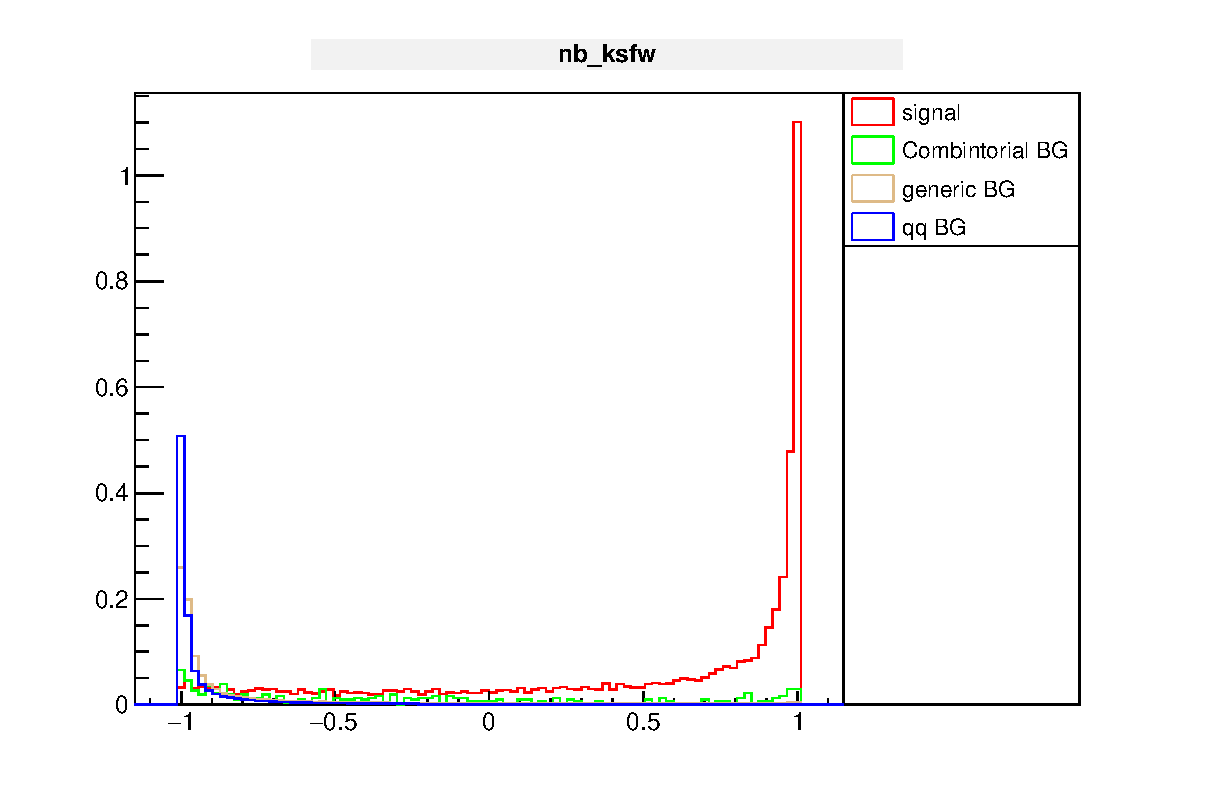
\includegraphics[width=0.45\textwidth]{bin_by_bin_study_figure/knunu/nb_ksfw_1025_1.eps}
		\label{knbksfw}
	}
	\subfigure[$K^{*\pm} \rightarrow K^\pm \pi^0$ mode.]{
		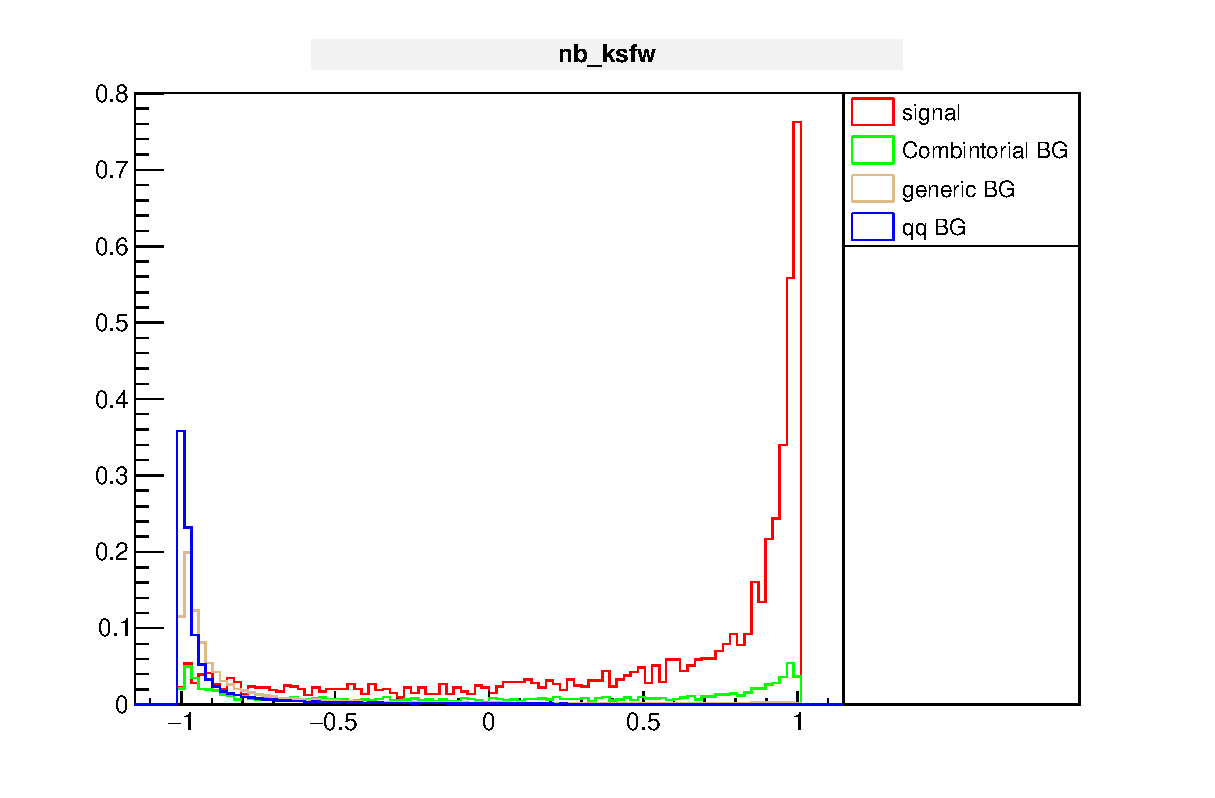
\includegraphics[width=0.45\textwidth]{bin_by_bin_study_figure/kstar1/nb_ksfw_1025_kstar1.eps}
		\label{kpi0nbksfw}
	}
	\subfigure[$K^{*\pm} \rightarrow K_s \pi^\pm$ mode.]{
		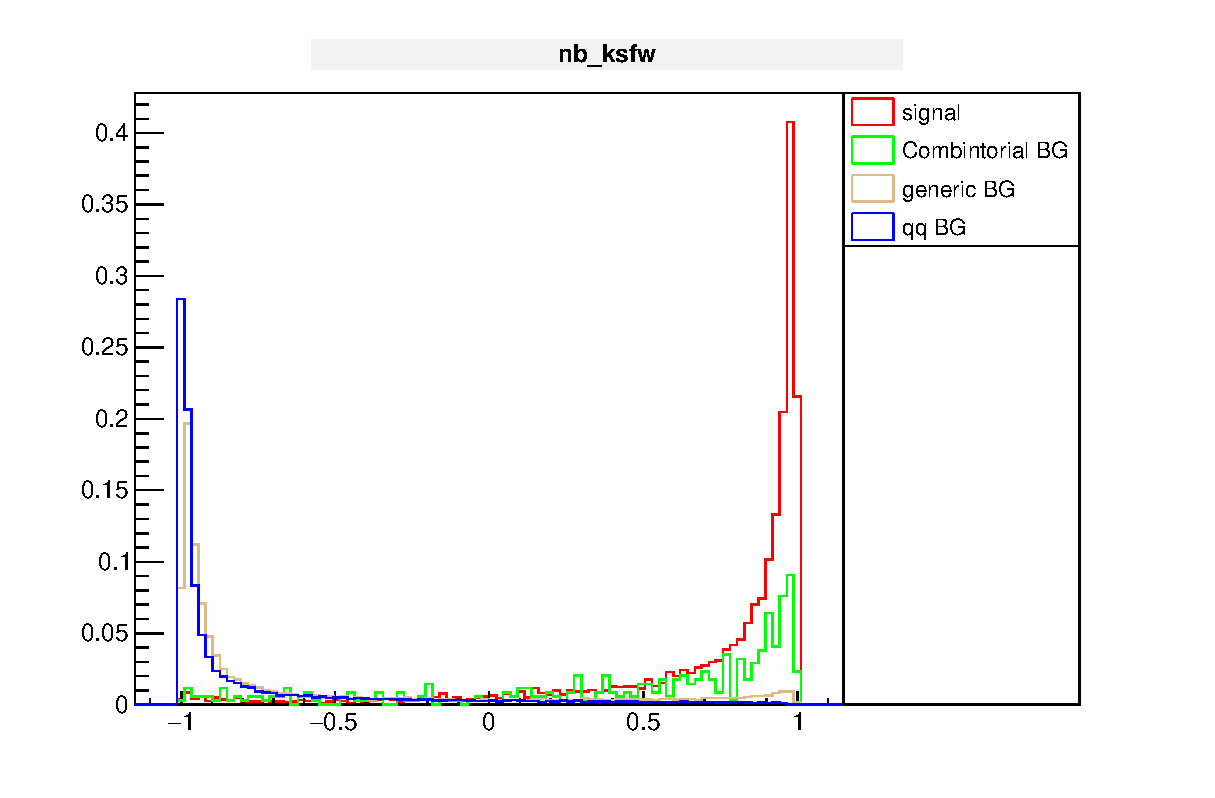
\includegraphics[width=0.45\textwidth]{bin_by_bin_study_figure/kstar2/nb_ksfw_1025_112.eps}
		\label{kspinbksfw}
	}
    \subfigure[$K^{*0}$ mode.]{
		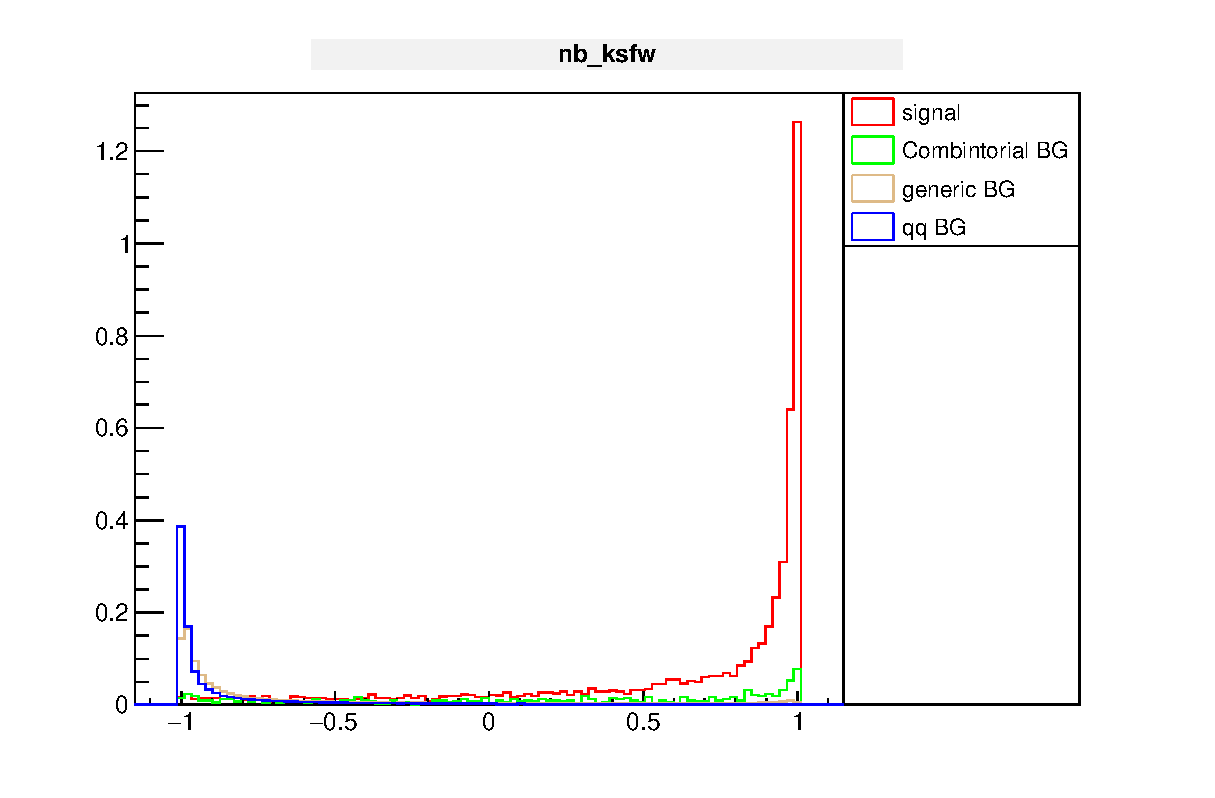
\includegraphics[width=0.45\textwidth]{bin_by_bin_study_figure/k0/nb_ksfw_1025_1.eps}
		\label{k0nbksfw}
	}
    \subfigure[$K_s$ mode.]{
		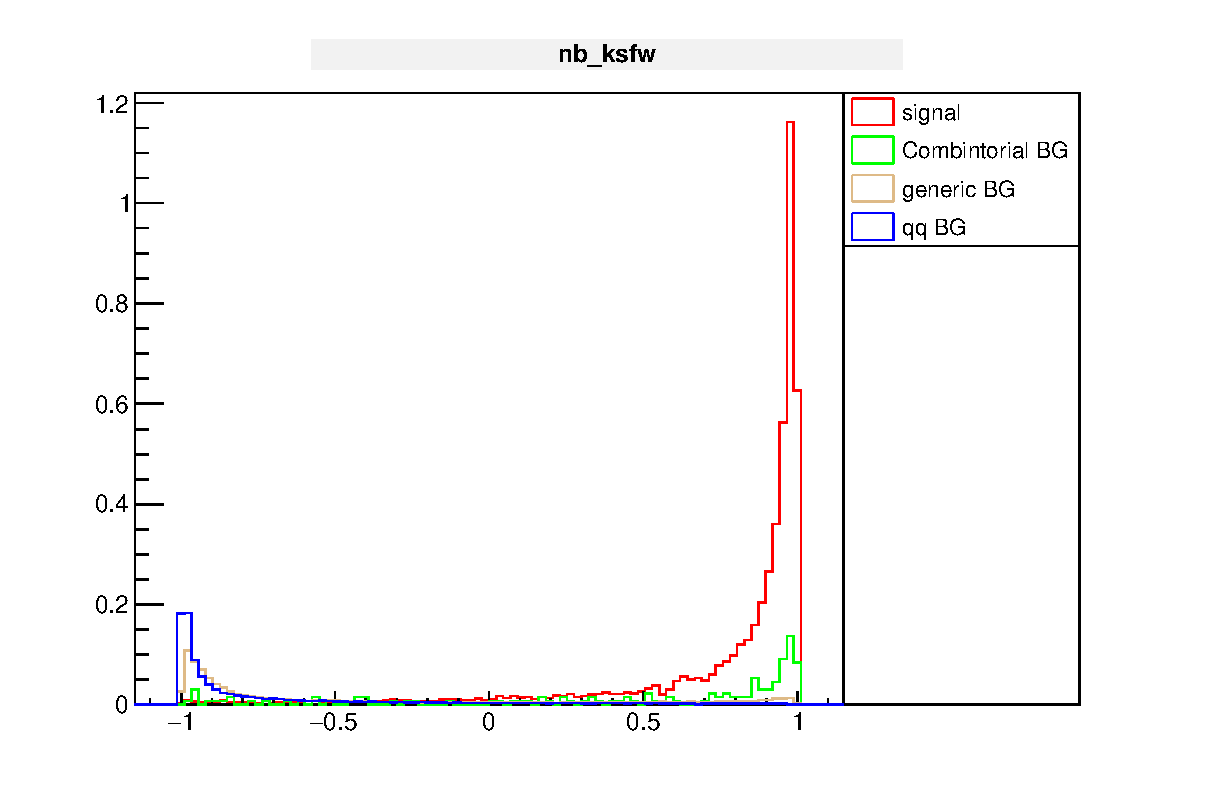
\includegraphics[width=0.45\textwidth]{bin_by_bin_study_figure/kshort/nb_ksfw_1025_1.eps}
		\label{ksnbksfw}
	}
\caption{Neurobayes output with KSFW variables for each mode. Red line represent signal, green line represent the combinatorial background,  brown line represent the generic background and blue line represent continuum background.}
\label{fig:nbksfw}	
\end{figure}

\subsection{Optimization}
With two different variables sets of training, we get two neural-network output, there are nbvlike(variables in \ref{t:nbvlike_variables}) and nbksfw(KSFW variables). We perform the two dimensional bin-by-bin optimization on $S_b$ distribution in the signal box, which $E_{ecl} < 0.3$ by maximizing the figure of merit\cite{ref:Punzi2003}
\begin{equation}
\label{eq:fom}
\mathcal{F.O.M} = \frac{\epsilon_{sig}}{0.5 n_{\sigma}+\sqrt{N_{bkg}}},
\end{equation}
where the number of sigmas $n_\sigma$ =1.28 corresponds to one-side Gaussian limit at 90 \% CL, $\epsilon_{sig}$ is signal efficiency and $N_{bkg}$ means the expected number of background events.\\
The partial signal efficiency means the signal efficiency found within the given $S_b$ interval multiplied by the fraction of the signal efficiency distribution inside that interval.
\begin{equation}
\label{eq:peff}
\epsilon^{'sig} = \frac{N_{yield}}{N_{gen} \times R_{bin} } 
\end{equation}
The $R_{bin}$ for each bin and each mode are shown in table \ref{t:rbin} and the original $S_b$ distribution without any selection for each mode are shown in fig \ref{fig:sbcmwithotcut}. 
% \begin{table}[ht]
% \small
% \begin{center}
% \begin{tabular}{ |p{0.8cm}||p{3.7cm}||p{1.2cm}||p{1.2cm}||p{2.6cm}||p{2.7cm}| }
%  \hline
%  Bin & Partial Signal Efficiency & nbvlike & nbksfw & $N_{sig}$ & $N_{bg}$  \\
%  \hline
%  bin 1  & $(8.97 \pm 0.24) \times 10^{-4}$ &0.8&0.7&$0.657\pm 0.018 $  &$0.0\pm 1.0 $\\ % &   $1.03 \times 10^{8}$&   $2.33 \times 10^{8}$ \\
%  \hline
%  bin 2  & $(9.90 \pm 0.27)\times 10^{-4}$ &0.6& -0.2&$0.653 \pm 0.017 $&$1.0\pm 1.0 $\\ % &   $1.03 \times 10^{8}$&   $2.33 \times 10^{8}$ \\
%  \hline
%  bin 3  & $(1.37 \pm 0.03)\times 10^{-3}$ &0.5&0.6&$0.796 \pm 0.019 $&$5.40\pm 2.32 $\\ % &   $1.03 \times 10^{8}$&   $2.33 \times 10^{8}$ \\
%  \hline
%  bin 4  & $(1.63 \pm 0.04)\times 10^{-3}$ &0.4&-0.5&$0.812 \pm 0.020 $&$19.4\pm 4.41 $ \\ % &   $1.03 \times 10^{8}$&   $2.33 \times 10^{8}$ \\
%  \hline
%  bin 5  & $(1.65\pm 0.04) \times 10^{-3}$ &0.3& -0.8&$0.687 \pm 0.018 $&$33.4\pm 5.78 $ \\ % &   $1.03 \times 10^{8}$&   $2.33 \times 10^{8}$ \\
%  \hline
%  bin 6  & $(1.51\pm 0.05) \times 10^{-3}$ &0.4& -0.8&$0.50\pm 0.015 $&$35.0 \pm 5.92 $\\ % &   $1.03 \times 10^{8}$&   $2.33 \times 10^{8}$ \\
%  \hline
%  bin 7  & $(1.73 \pm 0.06)\times 10^{-3}$ &0.2&-0.8&$0.419 \pm 0.014 $&$ 54.6\pm 7.39 $ \\ % &   $1.03 \times 10^{8}$&   $2.33 \times 10^{8}$ \\
%  \hline
%  bin 8  & $(1.19 \pm 0.06)\times 10^{-3}$ &0.3&-0.8&$0.166 \pm 0.009 $&$ 40.2\pm 6.34 $ \\ % &   $1.03 \times 10^{8}$&   $2.33 \times 10^{8}$ \\
%  \hline
%  bin 9  & $(1.25 \pm 0.14)\times 10^{-3}$ &-0.3&-0.9&$0.013 \pm 0.002 $&$ 2.4\pm 1.55 $ \\ % &   $1.03 \times 10^{8}$&   $2.33 \times 10^{8}$ \\
%  \hline
%  \hline
% \end{tabular}

% \caption{Bin-by-bin optimization in signal box $E_{ecl} < 0.3$ result for $B^\pm \rightarrow K^\pm \nu \bar{\nu}$, set 0.1 for a interval on $S_b$, use 5 stream of both bb and qq MC and rare MC. Optimize with nbvlike and nbksfw 2D cut } \label{t:optk}
% \end{center}
% \end{table}

\begin{table}[h]
\small
\begin{center}
\begin{tabular}{ |p{0.8cm}||p{3.7cm}||p{1.2cm}||p{1.2cm}||p{2.6cm}||p{2.7cm}| }
 \hline
 Bin & Partial Signal Efficiency & nbvlike & nbksfw & $N_{sig}$ & $N_{bg}$  \\
 \hline
 bin 1  & $(1.65 \pm 0.03) \times 10^{-3}$ &0.2&0.7&$1.21\pm 0.024 $  &$4.22\pm 2.05 $\\ % &   $1.03 \times 10^{8}$&   $2.33 \times 10^{8}$ \\
 \hline
 bin 2  & $(1.22 \pm 0.03)\times 10^{-3}$ &0.7& 0.3&$0.807 \pm 0.019 $&$3.3\pm 1.82 $\\ % &   $1.03 \times 10^{8}$&   $2.33 \times 10^{8}$ \\
 \hline
 bin 3  & $(1.37 \pm 0.03)\times 10^{-3}$ &0.5&0.6&$0.796 \pm 0.020 $&$6.66\pm 2.58 $\\ % &   $1.03 \times 10^{8}$&   $2.33 \times 10^{8}$ \\
 \hline
 bin 4  & $(1.63 \pm 0.04)\times 10^{-3}$ &0.4&-0.5&$0.812 \pm 0.020 $&$21.0\pm 4.58 $ \\ % &   $1.03 \times 10^{8}$&   $2.33 \times 10^{8}$ \\
 \hline
 bin 5  & $(1.65\pm 0.04) \times 10^{-3}$ &0.3& -0.8&$0.687 \pm 0.018 $&$35.06\pm 5.92 $ \\ % &   $1.03 \times 10^{8}$&   $2.33 \times 10^{8}$ \\
 \hline
 bin 6  & $(1.51\pm 0.05) \times 10^{-3}$ &0.4& -0.8&$0.50\pm 0.015 $&$36.46 \pm 6.04 $\\ % &   $1.03 \times 10^{8}$&   $2.33 \times 10^{8}$ \\
 \hline
 bin 7  & $(1.73 \pm 0.06)\times 10^{-3}$ &0.2&-0.8&$0.419 \pm 0.014 $&$ 56.08\pm 7.49 $ \\ % &   $1.03 \times 10^{8}$&   $2.33 \times 10^{8}$ \\
 \hline
 bin 8  & $(1.19 \pm 0.06)\times 10^{-3}$ &0.3&-0.8&$0.166 \pm 0.009 $&$ 41.04\pm 6.41 $ \\ % &   $1.03 \times 10^{8}$&   $2.33 \times 10^{8}$ \\
 \hline
 bin 9  & $(1.25 \pm 0.14)\times 10^{-3}$ &-0.3&-0.9&$0.013 \pm 0.002 $&$ 2.44\pm 1.56 $ \\ % &   $1.03 \times 10^{8}$&   $2.33 \times 10^{8}$ \\
 \hline
 \hline
\end{tabular}

\caption{Bin-by-bin optimization in signal box $E_{ecl} < 0.3$ result for $B^\pm \rightarrow K^\pm \nu \bar{\nu}$, set 0.1 for a interval on $S_b$, use 5 stream of both bb and qq MC and rare MC. Optimize with nbvlike and nbksfw 2D cut } \label{t:optk}
\end{center}
\end{table}

\begin{table}[h]
\small
\begin{center}
\begin{tabu}to \textwidth{ |X[l]|X[c]|X[c]|X[c]|X[c]| }
\hline
 Bin & $N_{BG}$ &$N_{generic BG}$ & $N_{continuum BG}$ & $N_{rare BG}$   \\
 \hline
 bin 1  & 4.22  &0.2 &1.0&3.02\\ 
 \hline
 bin 2  & 3.3  &1.8 &0.4&1.1\\ 
 \hline
 bin 3  & 6.66  &4.6 &0.0&1.26\\ 
 \hline
 bin 4  & 21.0 	&17.8 &1.6&1.6 \\ 
 \hline
 bin 5  & 35.06  &29.2 &2.0&1.66 \\ 
 \hline
 bin 6  & 36.46 &31.6 &1.2&1.46 \\
 \hline
 bin 7  & 56.08 	&45.2 &0.6&1.48 \\ 
 \hline
  bin 8  & 41.04 	&32.2 &0.2&0.84 \\ 
 \hline
  bin 9  & 2.44 	&1.8 &0.2&0.04 \\ 
 \hline
 \hline
\end{tabu}
\caption{Background composition for $B^\pm \rightarrow K^\pm \nu \bar{\nu}$,, all the amount are scale to one data size.} \label{t:bgcomk}
\end{center}
\end{table}


\begin{figure}[ht]
\centering
\subfigure[Bin1]{
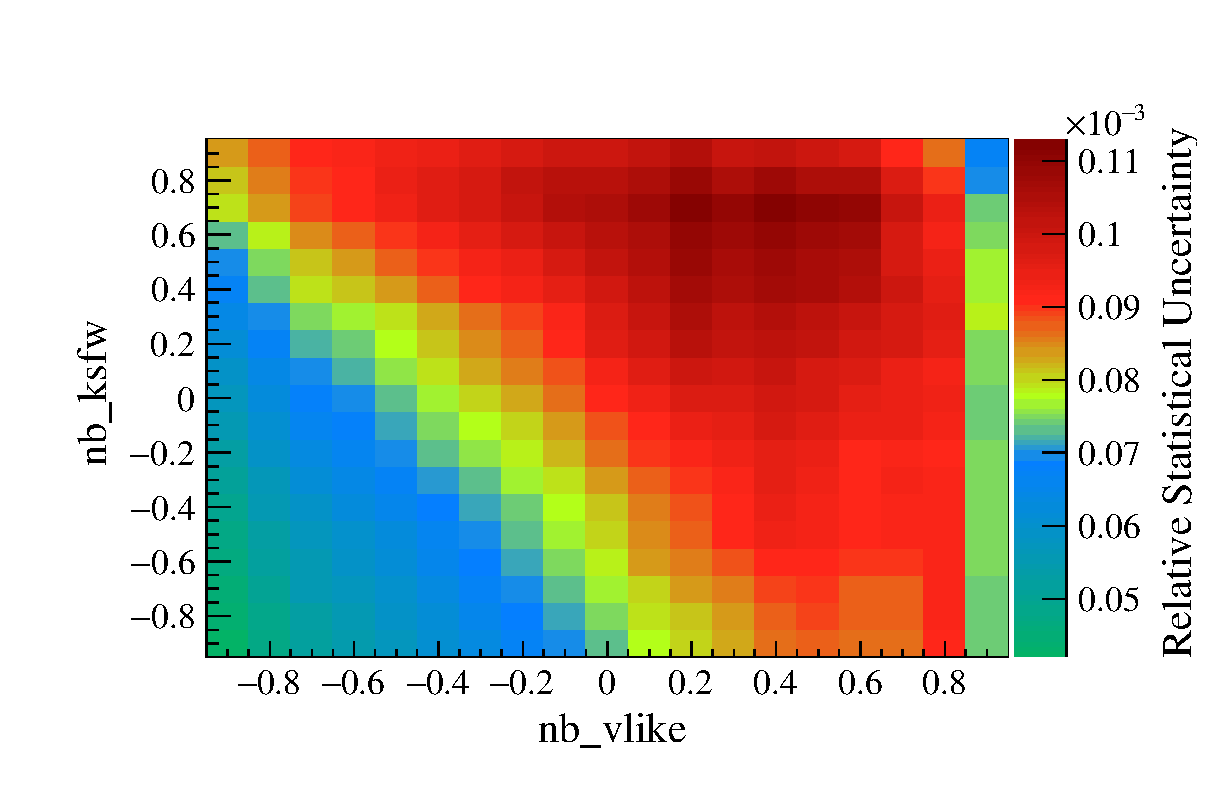
\includegraphics[width=0.2\textwidth]{bin_by_bin_study_figure/knunu/Uncert_0_1118_01bin.eps}
\label{kbin1}
}
    \subfigure[Bin2]{
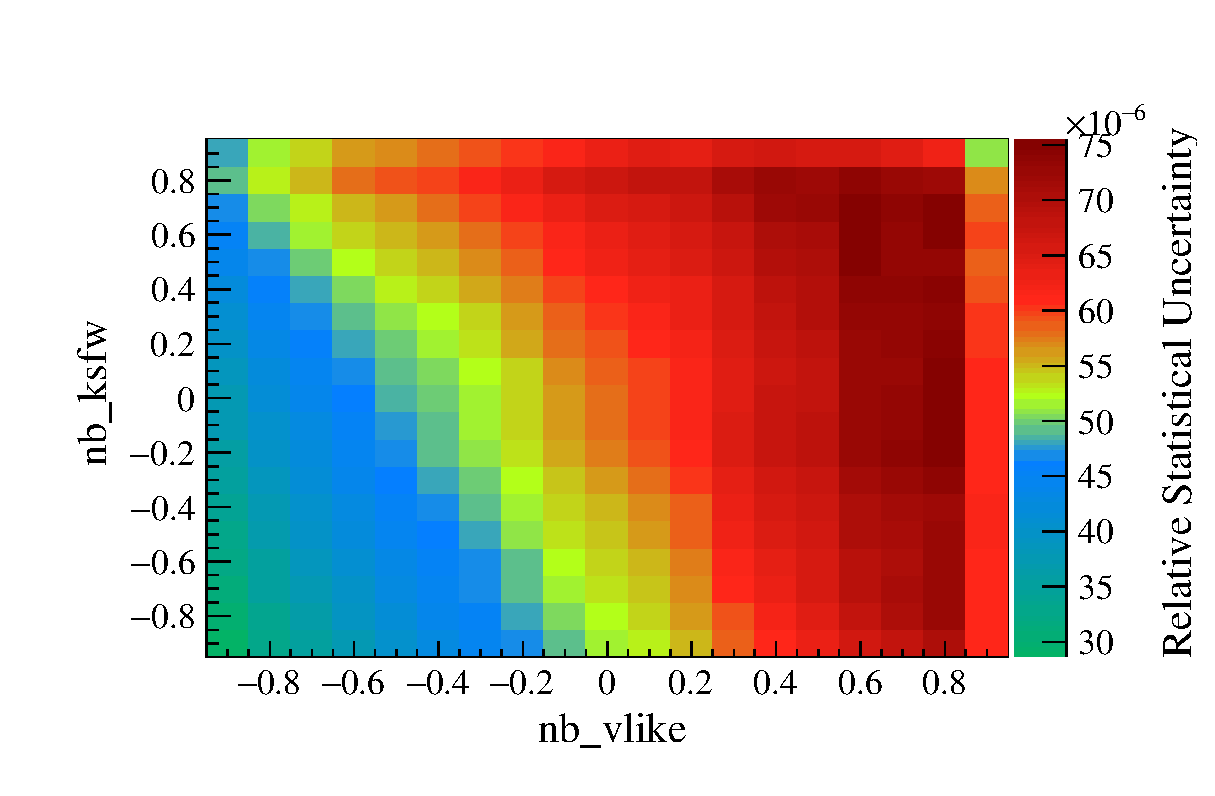
\includegraphics[width=0.2\textwidth]{bin_by_bin_study_figure/knunu/Uncert_1_1118_01bin.eps}
\label{kbin2}
	}
    \subfigure[Bin3]{
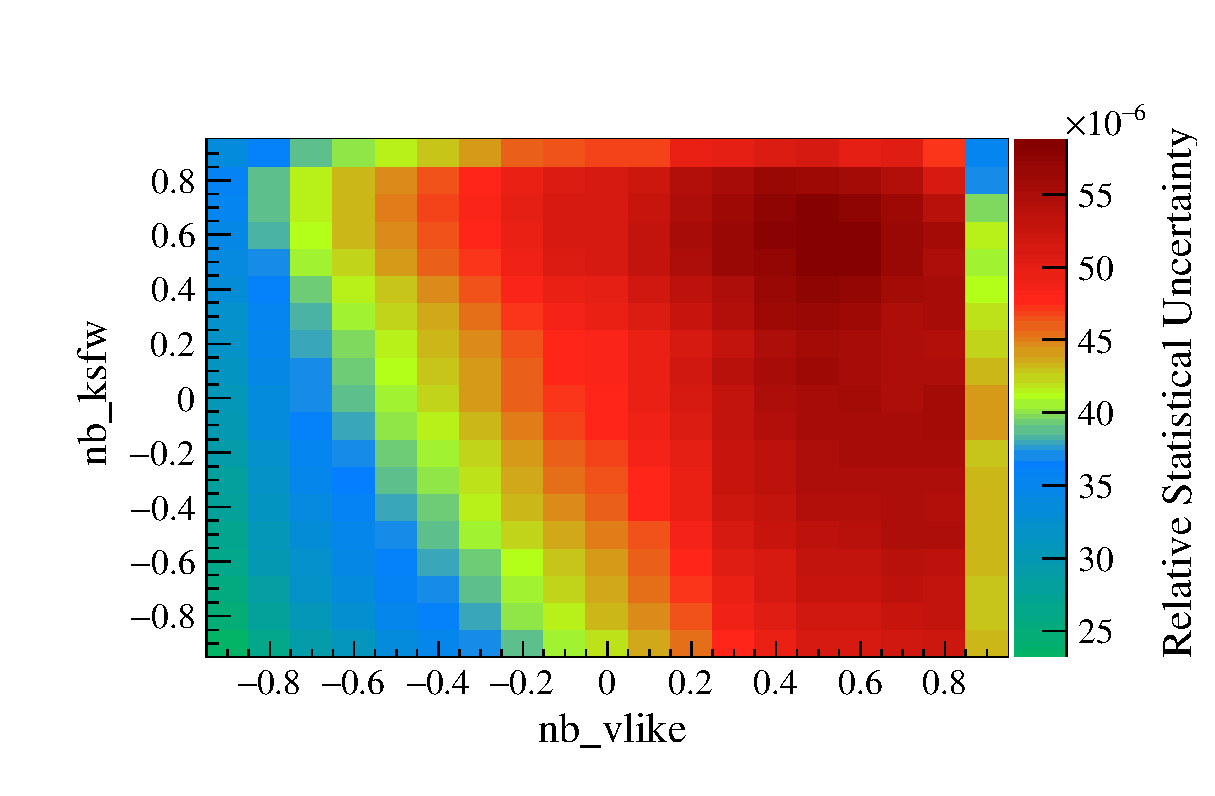
\includegraphics[width=0.2\textwidth]{bin_by_bin_study_figure/knunu/Uncert_2_1118_01bin.eps}
\label{kbin3}
	}
    \subfigure[Bin4]{
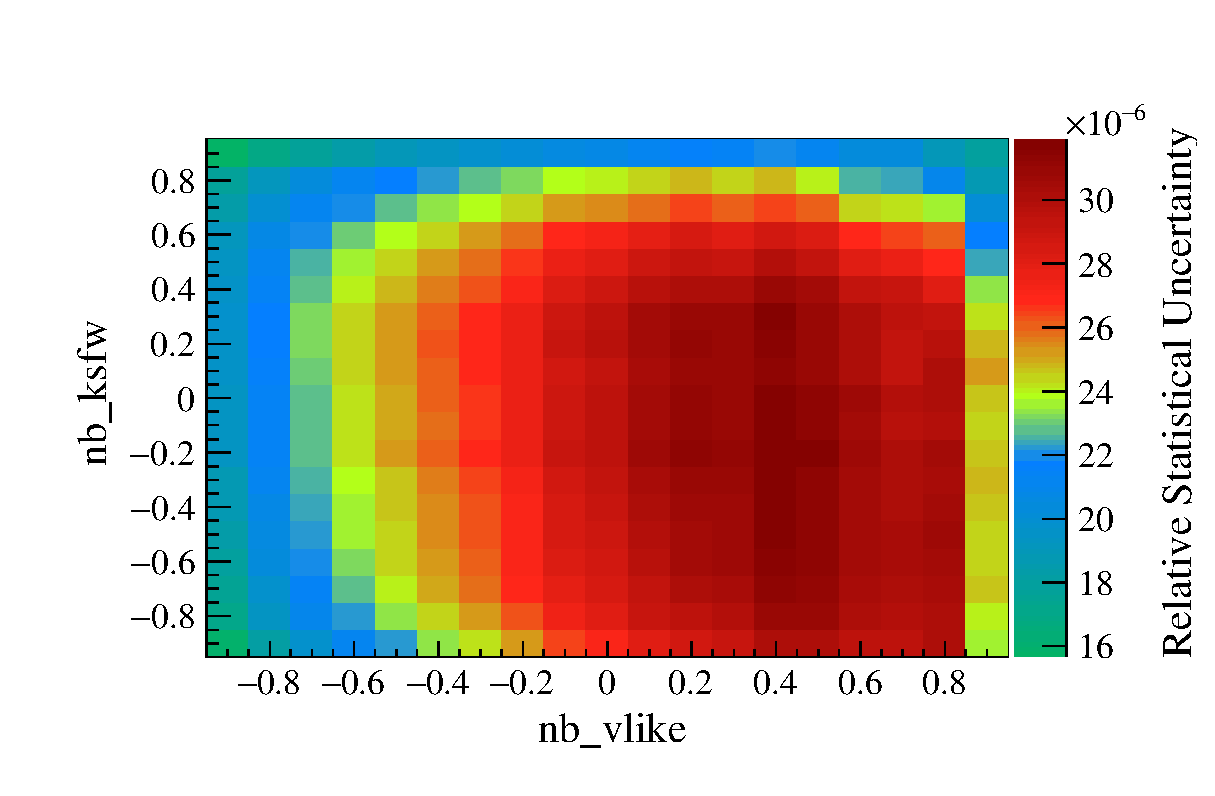
\includegraphics[width=0.2\textwidth]{bin_by_bin_study_figure/knunu/Uncert_3_1118_01bin.eps}
\label{kbin4}
	}
    \subfigure[Bin5]{
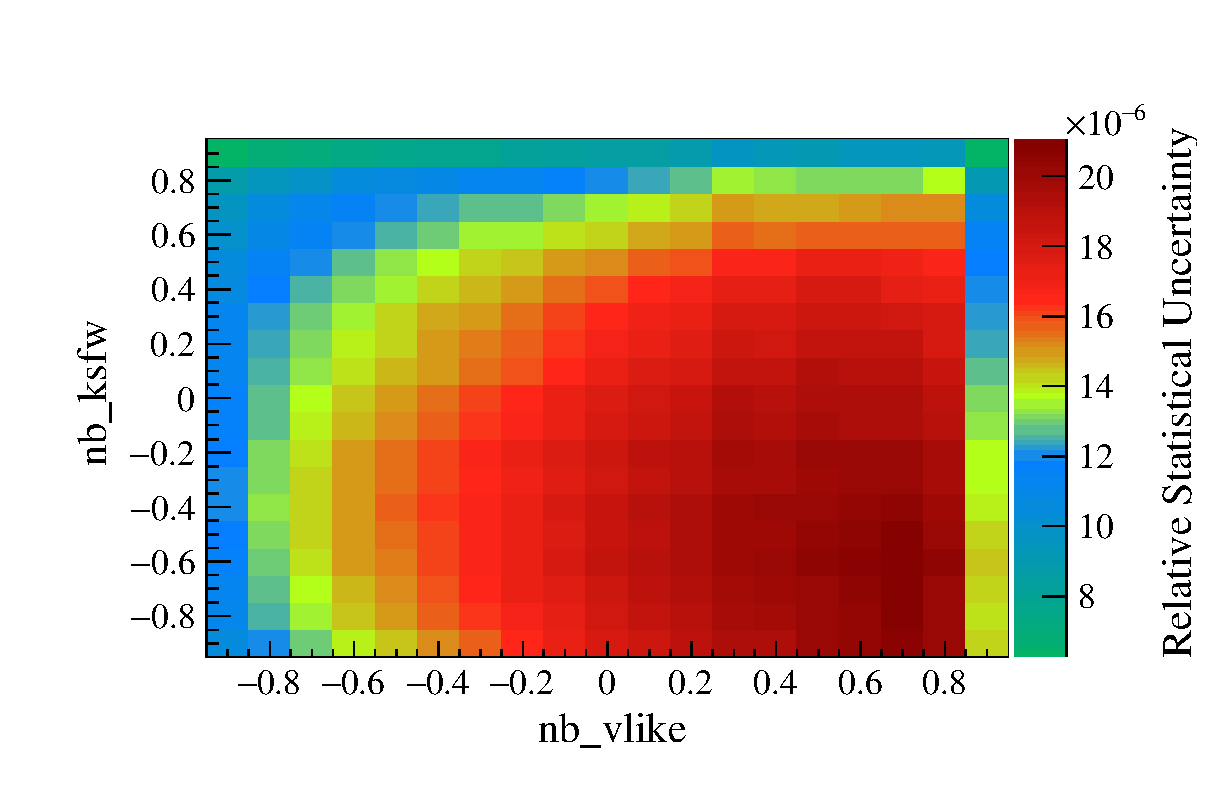
\includegraphics[width=0.2\textwidth]{bin_by_bin_study_figure/knunu/Uncert_4_1118_01bin.eps}
\label{kbin5}
	}
    \subfigure[Bin6]{
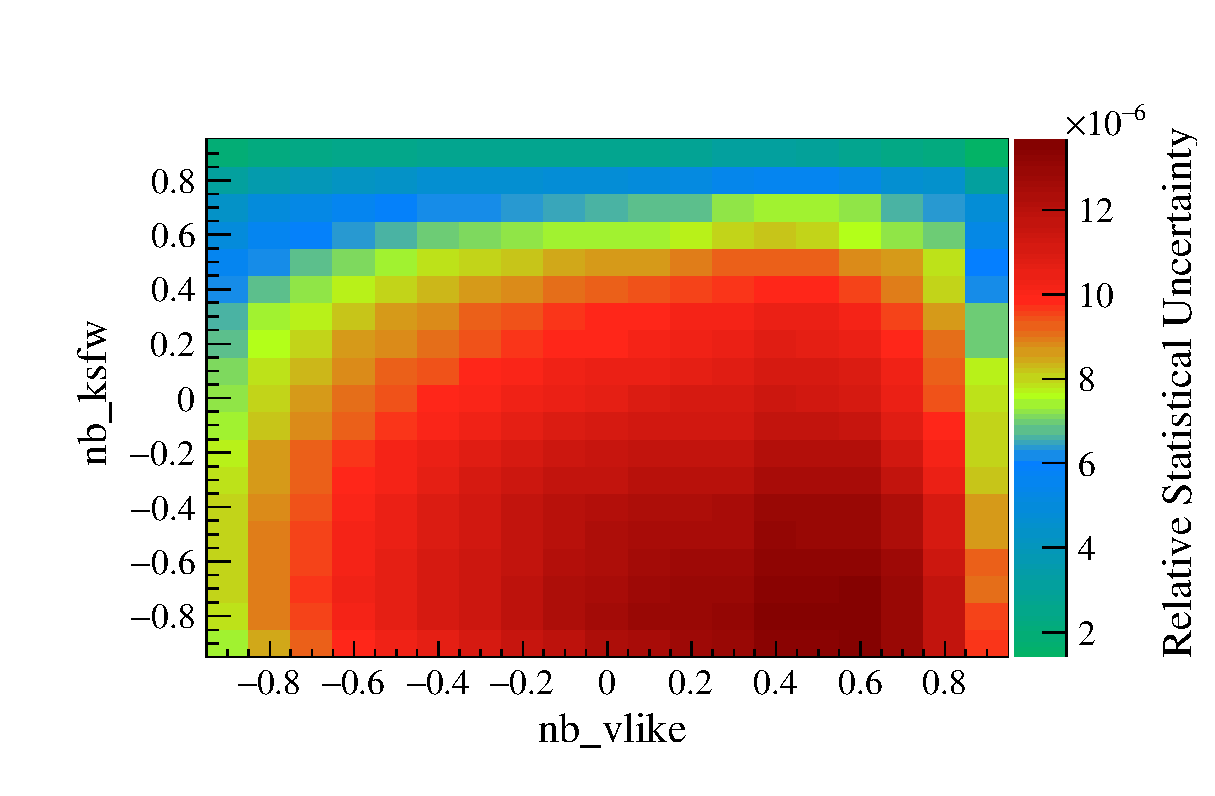
\includegraphics[width=0.2\textwidth]{bin_by_bin_study_figure/knunu/Uncert_5_1118_01bin.eps}
\label{kbin6}
	}
    \subfigure[Bin7]{
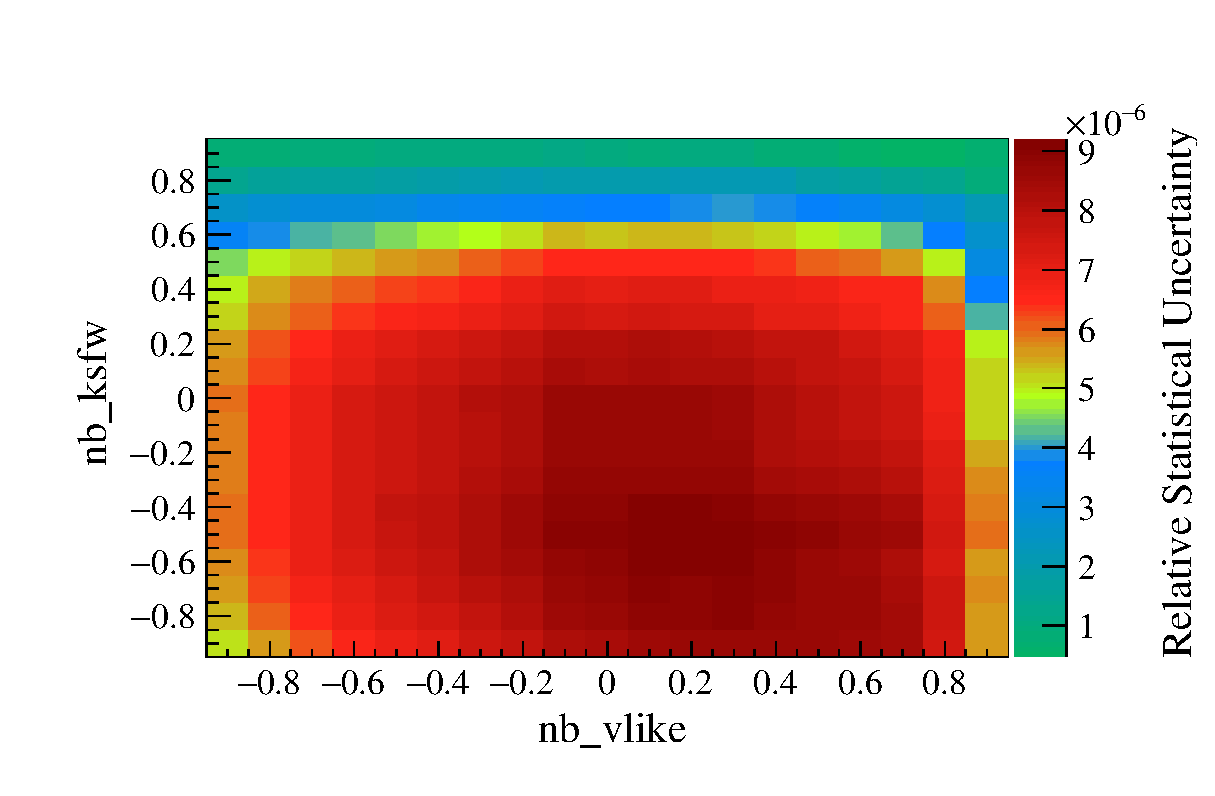
\includegraphics[width=0.2\textwidth]{bin_by_bin_study_figure/knunu/Uncert_6_1118_01bin.eps}
\label{kbin7}
	}
    \subfigure[Bin8]{
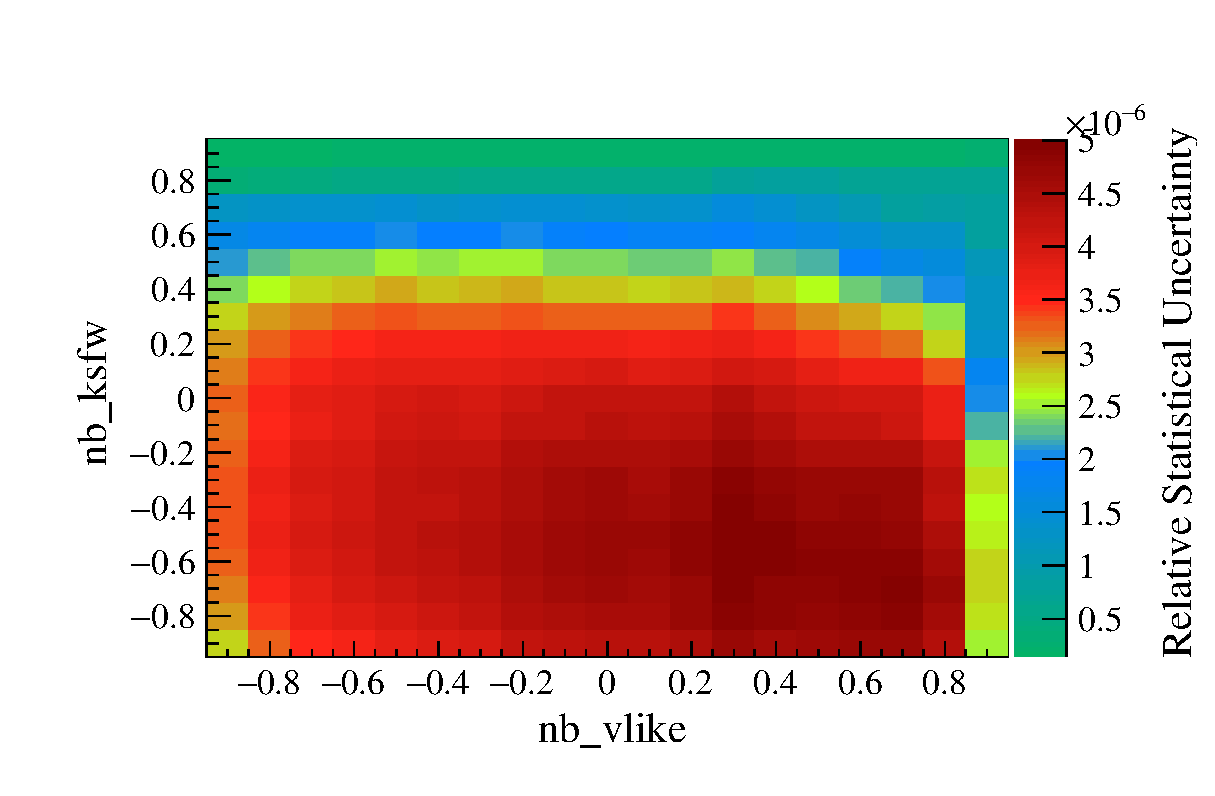
\includegraphics[width=0.2\textwidth]{bin_by_bin_study_figure/knunu/Uncert_7_1118_01bin.eps}
\label{kbin8}
	}
    \subfigure[Bin9]{
\includegraphics[width=0.2\textwidth]{bin_by_bin_study_figure/knunu/Uncert_8_1118_01bin.eps}
\label{kbin9}
	}
\caption{Two dimensional bin-by-bin $\mathcal{F.O.M.}$ plot for $B^\pm \rightarrow K^\pm \nu \bar{\nu}$.}
\label{fig:binbybinoptk}	
\end{figure}

\begin{table}[h]
\small
\begin{center}
\begin{tabular}{ |p{0.8cm}||p{3.7cm}||p{1.2cm}||p{1.2cm}||p{2.6cm}||p{2.7cm}| }
  \hline
 Bin & Partial Signal Efficiency & nbvlike & nbksfw & $N_{sig}$ & $N_{bg}$  \\
 \hline
 bin 1  & $(1.43 \pm 0.09) \times 10^{-4}$ &0.0&0.6&$0.26\pm 0.005 $  &$1.47\pm 1.21 $\\ % &   $1.03 \times 10^{8}$&   $2.33 \times 10^{8}$ \\
 \hline
 bin 2  & $(1.26 \pm 0.09)\times 10^{-4}$ &0.5& -0.9&$0.166 \pm 0.004 $&$1.57\pm 1.25 $\\ % &   $1.03 \times 10^{8}$&   $2.33 \times 10^{8}$ \\
 \hline
 bin 3  & $(1.18 \pm 0.09)\times 10^{-4}$ &0.2&0.1&$0.12 \pm 0.004 $&$1.97\pm 1.4 $\\ % &   $1.03 \times 10^{8}$&   $2.33 \times 10^{8}$ \\
 \hline
 bin 4  & $(1.20 \pm 0.10)\times 10^{-4}$ &0.1&-0.7&$0.14 \pm 0.004 $&$5.34\pm 2.31 $ \\ % &   $1.03 \times 10^{8}$&   $2.33 \times 10^{8}$ \\
 \hline
 bin 5  & $(1.11\pm 0.11) \times 10^{-4}$ &0.0& -0.9&$0.0995 \pm 0.003 $&$7.64\pm 2.76 $ \\ % &   $1.03 \times 10^{8}$&   $2.33 \times 10^{8}$ \\
 \hline
 bin 6  & $(1.18\pm 0.14) \times 10^{-4}$ &-0.6& -0.9&$0.078\pm 0.003 $&$21.97 \pm 4.69 $\\ % &   $1.03 \times 10^{8}$&   $2.33 \times 10^{8}$ \\
 \hline
 bin 7  & $(3.73 \pm 1.14)\times 10^{-5}$ &-0.1&0.2&$0.0109 \pm 0.001 $&$ 2.4\pm 1.55 $ \\ % &   $1.03 \times 10^{8}$&   $2.33 \times 10^{8}$ \\
 \hline
 \hline
\end{tabular}

\caption{Bin-by-bin optimization in signal box $E_{ecl} < 0.3$ result for $K^{*\pm} \rightarrow K^{+} \pi^0$, set 0.1 for a interval on $S_b$, use 5 stream of both bb and qq MC and rare MC. Optimize with nbvlike and nbksfw 2D cut } \label{t:optkpi0}
\end{center}
\end{table}

\begin{table}[h]
\small
\begin{center}
\begin{tabu}to \textwidth{ |X[l]|X[c]|X[c]|X[c]|X[c]| }
\hline
 Bin & $N_{BG}$ &$N_{generic BG}$ & $N_{continuum BG}$ & $N_{rare BG}$   \\
 \hline
 bin 1  & 1.47  &0 &0.2&1.26\\ 
 \hline
 bin 2  & 1.57  &1.0 &0.2&0.36\\ 
 \hline
 bin 3  & 1.97  &1.0 &0.4&0.56\\ 
 \hline
 bin 4  & 5.34 	&4.4 &0.4&0.52 \\ 
 \hline
 bin 5  & 7.64  &7 &0.2&0.42 \\ 
 \hline
 bin 6  & 21.97 &19.2 &2.2&0.54 \\
 \hline
 bin 7  & 2.4 	&2.2 &0.2&0.04 \\ 
 \hline
 \hline
\end{tabu}
\caption{Background composition for $K^* \rightarrow K \pi^0$, all the amount are scale to one data size.} \label{t:bgcomkpi0}
\end{center}
\end{table}




% \begin{table}[h]
% \small
% \begin{center}
% \begin{tabular}{ |p{0.8cm}||p{3.7cm}||p{1.2cm}||p{1.2cm}||p{2.6cm}||p{2.7cm}| }
%   \hline
%  Bin & Partial Signal Efficiency & nbvlike & nbksfw & $N_{sig}$ & $N_{bg}$  \\
%  \hline
%  bin 1  & $(1.43 \pm 0.09) \times 10^{-4}$ &0.0&0.6&$0.26\pm 0.005 $  &$0.21\pm 0.458 $\\ % &   $1.03 \times 10^{8}$&   $2.33 \times 10^{8}$ \\
%  \hline
%  bin 2  & $(1.03 \pm 0.08)\times 10^{-4}$ &0.6& 0.5&$0.166 \pm 0.004 $&$0.606\pm 0.778 $\\ % &   $1.03 \times 10^{8}$&   $2.33 \times 10^{8}$ \\
%  \hline
%  bin 3  & $(8.59 \pm 0.80)\times 10^{-5}$ &0.2&0.8&$0.12 \pm 0.004 $&$0.41\pm 0.64 $\\ % &   $1.03 \times 10^{8}$&   $2.33 \times 10^{8}$ \\
%  \hline
%  bin 4  & $(1.20 \pm 0.10)\times 10^{-4}$ &0.1&-0.7&$0.14 \pm 0.004 $&$4.8\pm 2.19 $ \\ % &   $1.03 \times 10^{8}$&   $2.33 \times 10^{8}$ \\
%  \hline
%  bin 5  & $(1.07\pm 0.11) \times 10^{-4}$ &0.0& -0.9&$0.0995 \pm 0.003 $&$7.22\pm 2.69 $ \\ % &   $1.03 \times 10^{8}$&   $2.33 \times 10^{8}$ \\
%  \hline
%  bin 6  & $(1.18\pm 0.14) \times 10^{-4}$ &-0.6& -0.9&$0.078\pm 0.003 $&$21.43 \pm 4.63 $\\ % &   $1.03 \times 10^{8}$&   $2.33 \times 10^{8}$ \\
%  \hline
%  bin 7  & $(3.73 \pm 1.10)\times 10^{-5}$ &-0.1&0.2&$0.0109 \pm 0.001 $&$ 2.4\pm 1.55 $ \\ % &   $1.03 \times 10^{8}$&   $2.33 \times 10^{8}$ \\
%  \hline
%  \hline
% \end{tabular}

% \caption{Bin-by-bin optimization in signal box $E_{ecl} < 0.3$ result for $K^{*\pm} \rightarrow K^{+} \pi^0$, set 0.1 for a interval on $S_b$, use 5 stream of both bb and qq MC. Optimize with nbvlike and nbksfw 2D cut } \label{t:optkpi0}
% \end{center}
% \end{table}

\begin{figure}[ht]
\centering
\subfigure[Bin1]{
\includegraphics[width=0.2\textwidth]{bin_by_bin_study_figure/kstar1/Uncert_0_1118_01bin.eps}
\label{kpi0bin1}
}
    \subfigure[Bin2]{
\includegraphics[width=0.2\textwidth]{bin_by_bin_study_figure/kstar1/Uncert_1_1118_01bin.eps}
\label{kpi0bin2}
	}
    \subfigure[Bin3]{
\includegraphics[width=0.2\textwidth]{bin_by_bin_study_figure/kstar1/Uncert_2_1118_01bin.eps}
\label{kpi0bin3}
	}
    \subfigure[Bin4]{
\includegraphics[width=0.2\textwidth]{bin_by_bin_study_figure/kstar1/Uncert_3_1118_01bin.eps}
\label{kpi0bin4}
	}
    \subfigure[Bin5]{
\includegraphics[width=0.2\textwidth]{bin_by_bin_study_figure/kstar1/Uncert_4_1118_01bin.eps}
\label{kpi0bin5}
	}
    \subfigure[Bin6]{
\includegraphics[width=0.2\textwidth]{bin_by_bin_study_figure/kstar1/Uncert_5_1118_01bin.eps}
\label{kpi0bin6}
	}
    \subfigure[Bin7]{
\includegraphics[width=0.2\textwidth]{bin_by_bin_study_figure/kstar1/Uncert_6_1118_01bin.eps}
\label{kpi0bin7}
	}
\caption{Two dimensional bin-by-bin $\mathcal{F.O.M.}$ plot for $K^{*\pm} \rightarrow K^{+} \pi^0$ .}
\label{fig:binbybinoptkpi0}	
\end{figure}

% \begin{table}[ht]
% \small
% \begin{center}
% \begin{tabular}{ |p{0.8cm}||p{3.7cm}||p{1.2cm}||p{1.2cm}||p{2.6cm}||p{2.7cm}| }
%  \hline
%  Bin & Signal Efficiency & nbvlike & nbksfw & $N_{sig}$ & $N_{bg}$  \\
%  \hline
%  bin 1  & $(1.32 \pm 0.086) \times 10^{-4}$ &0.9&0.7&$0.24\pm 0.004 $  &$0.0002\pm 0.016 $\\ % &   $1.03 \times 10^{8}$&   $2.33 \times 10^{8}$ \\
%  \hline
%  bin 2  & $(2.21 \pm 0.012)\times 10^{-4}$ &0.3& 0.6&$0.357 \pm 0.004 $&$1.80\pm 1.34 $\\ % &   $1.03 \times 10^{8}$&   $2.33 \times 10^{8}$ \\
%  \hline
%  bin 3  & $(1.96 \pm 0.012)\times 10^{-4}$ &0.7&-0.5&$0.274 \pm 0.003 $&$1.60\pm 1.26 $\\ % &   $1.03 \times 10^{8}$&   $2.33 \times 10^{8}$ \\
%  \hline
%  bin 4  & $(1.78 \pm 0.012)\times 10^{-4}$ &0.5&-0.1&$0.208 \pm 0.003 $&$3.80\pm 1.95 $ \\ % &   $1.03 \times 10^{8}$&   $2.33 \times 10^{8}$ \\
%  \hline
%  bin 5  & $(1.28\pm 0.12) \times 10^{-4}$ &0.8& -0.5&$0.119 \pm 0.003 $&$3.20\pm 1.79 $ \\ % &   $1.03 \times 10^{8}$&   $2.33 \times 10^{8}$ \\
%  \hline
%  bin 6  & $(1.11\pm 0.13) \times 10^{-4}$ &0.8& 0.1&$0.073\pm 0.002 $&$2.40 \pm 1.55 $\\ % &   $1.03 \times 10^{8}$&   $2.33 \times 10^{8}$ \\
%  \hline
%  bin 7  & $(6.3 \pm 1.0)\times 10^{-5}$ &0.7&-0.9&$0.035 \pm 0.001 $&$ 2.60\pm 1.61 $ \\ % &   $1.03 \times 10^{8}$&   $2.33 \times 10^{8}$ \\
%  \hline
%  \hline
% \end{tabular}

% \caption{Bin-by-bin optimization in signal box $E_{ecl} < 0.3$ result for $K^* \rightarrow K_s \pi^+$, set 0.1 for a interval on $S_b$, use 5 stream of both bb and qq MC. Optimize with nbvlike and nbksfw 2D cut } \label{t:optkspi}
% \end{center}
% \end{table}
\clearpage

\begin{table}[h]
\small
\begin{center}
\begin{tabular}{ |p{0.8cm}||p{3.7cm}||p{1.2cm}||p{1.2cm}||p{2.6cm}||p{2.7cm}| }
 \hline
 Bin & Signal Efficiency & nbvlike & nbksfw & $N_{sig}$ & $N_{bg}$  \\
 \hline
 bin 1  & $(2.54 \pm 0.12) \times 10^{-4}$ &0.4&0.6&$0.46\pm 0.005 $  &$2.34\pm 1.53 $\\ % &   $1.03 \times 10^{8}$&   $2.33 \times 10^{8}$ \\
 \hline
 bin 2  & $(2.38 \pm 0.12)\times 10^{-4}$ &0.2& 0.8&$0.385 \pm 0.004 $&$2.54\pm 1.59 $\\ % &   $1.03 \times 10^{8}$&   $2.33 \times 10^{8}$ \\
 \hline
 bin 3  & $(2.41 \pm 0.13)\times 10^{-4}$ &0.6&-0.1&$0.337 \pm 0.003 $&$2.98\pm 1.73 $\\ % &   $1.03 \times 10^{8}$&   $2.33 \times 10^{8}$ \\
 \hline
 bin 4  & $(1.99 \pm 0.13)\times 10^{-4}$ &0.6&0.0&$0.233 \pm 0.002 $&$4.48\pm 2.11 $ \\ % &   $1.03 \times 10^{8}$&   $2.33 \times 10^{8}$ \\
 \hline
 bin 5  & $(1.58\pm 0.13) \times 10^{-4}$ &0.8& -0.5&$0.147 \pm 0.001 $&$4.66\pm 2.16 $ \\ % &   $1.03 \times 10^{8}$&   $2.33 \times 10^{8}$ \\
 \hline
 bin 6  & $(1.34\pm 0.14) \times 10^{-4}$ &0.8& -0.1&$0.088\pm 0.001 $&$4.24 \pm 2.06 $\\ % &   $1.03 \times 10^{8}$&   $2.33 \times 10^{8}$ \\
 \hline
 bin 7  & $(8.35 \pm 1.24)\times 10^{-5}$ &0.4&-0.6&$0.046 \pm 0.0004 $&$ 4.08\pm 2.02 $ \\ % &   $1.03 \times 10^{8}$&   $2.33 \times 10^{8}$ \\
 \hline
 \hline
\end{tabular}

\caption{Bin-by-bin optimization in signal box $E_{ecl} < 0.3$ result for $K^* \rightarrow K_s \pi^+$, set 0.1 for a interval on $S_b$, use 5 stream of both bb and qq MC and rare MC. Optimize with nbvlike and nbksfw 2D cut } \label{t:optkspi}
\end{center}
\end{table}

\begin{table}[h]
\small
\begin{center}
\begin{tabu}to \textwidth{ |X[l]|X[c]|X[c]|X[c]|X[c]| }
\hline
 Bin & $N_{BG}$ &$N_{generic BG}$ & $N_{continuum BG}$ & $N_{rare BG}$   \\
 \hline
 bin 1  & 2.34  &0.2 &1.0&1.14\\ 
 \hline
 bin 2  & 2.54  &1.4 &0.4&0.74\\ 
 \hline
 bin 3  & 2.98  &1.6 &0.8&0.58\\ 
 \hline
 bin 4  & 4.48 	&3.2 &0.8&0.48 \\ 
 \hline
 bin 5  & 4.66  &3.8 &0.6&0.26 \\ 
 \hline
 bin 6  & 4.24 	&3.4 &0.6&0.24 \\
 \hline
 bin 7  & 4.08 	&3.4 &0.6&0.08 \\ 
 \hline
 \hline
\end{tabu}
\caption{Background composition for $K^* \rightarrow K_s \pi^+$, all the amount are scale to one data size.} \label{t:bgcomkspi}
\end{center}
\end{table}






\begin{figure}[ht]
\centering
\subfigure[Bin1]{
\includegraphics[width=0.2\textwidth]{bin_by_bin_study_figure/kstar2/Uncert_0_1118_01bin11.eps}
\label{kspibin1}
}
\subfigure[Bin2]{
\includegraphics[width=0.2\textwidth]{bin_by_bin_study_figure/kstar2/Uncert_1_1118_01bin11.eps}
\label{kspibin2}
}
\subfigure[Bin3]{
\includegraphics[width=0.2\textwidth]{bin_by_bin_study_figure/kstar2/Uncert_2_1118_01bin11.eps}
\label{kspibin3}
}
\subfigure[Bin4]{
\includegraphics[width=0.2\textwidth]{bin_by_bin_study_figure/kstar2/Uncert_3_1118_01bin11.eps}
\label{kspibin4}
}
\subfigure[Bin5]{
\includegraphics[width=0.2\textwidth]{bin_by_bin_study_figure/kstar2/Uncert_4_1118_01bin11.eps}
\label{kspibin5}
}
\subfigure[Bin6]{
\includegraphics[width=0.2\textwidth]{bin_by_bin_study_figure/kstar2/Uncert_5_1118_01bin11.eps}
\label{kspibin6}
}
\subfigure[Bin7]{
\includegraphics[width=0.2\textwidth]{bin_by_bin_study_figure/kstar2/Uncert_6_1118_01bin11.eps}
\label{kspibin7}
}
\caption{Two dimensional bin-by-bin $\mathcal{F.O.M.}$ plot for $K^{*\pm} \rightarrow K_s \pi^+$ .}
\label{fig:binbybinoptkspi}	
\end{figure}

\begin{table}[h]
\small
\begin{center}
\begin{tabular}{ |p{0.8cm}||p{3.7cm}||p{1.2cm}||p{1.2cm}||p{2.6cm}||p{2.7cm}| }
\hline
 Bin & Signal Efficiency & nbvlike & nbksfw & $N_{sig}$ & $N_{bg}$  \\
 \hline
 bin 1  & $(6.01 \pm 0.183) \times 10^{-4}$ &-0.2&0.5&$1.02\pm 0.015 $  &$9.84\pm 3.14 $\\ % &   $1.03 \times 10^{8}$&   $2.33 \times 10^{8}$ \\
 \hline
 bin 2  & $(5.22 \pm 0.182)\times 10^{-4}$ &0.2& 0.0&$0.784 \pm 0.012 $&$6.0\pm 2.45 $\\ % &   $1.03 \times 10^{8}$&   $2.33 \times 10^{8}$ \\
 \hline
 bin 3  & $(4.03 \pm 0.172)\times 10^{-4}$ &0.7&-0.3&$0.522 \pm 0.009 $&$3.64\pm 1.91 $\\ % &   $1.03 \times 10^{8}$&   $2.33 \times 10^{8}$ \\
 \hline
 bin 4  & $(4.82 \pm 0.206)\times 10^{-4}$ &0.2&0.0&$0.522 \pm 0.009 $&$16.28\pm 4.03 $ \\ % &   $1.03 \times 10^{8}$&   $2.33 \times 10^{8}$ \\
 \hline
 bin 5  & $(3.08\pm 0.184) \times 10^{-4}$ &0.8& 0.2&$0.264 \pm 0.002 $&$5.0\pm 2.24 $ \\ % &   $1.03 \times 10^{8}$&   $2.33 \times 10^{8}$ \\
 \hline
 bin 6  & $(4.44\pm 0.26) \times 10^{-4}$ &0.3& -0.6&$0.269\pm 0.005 $&$24.34 \pm 4.93 $\\ % &   $1.03 \times 10^{8}$&   $2.33 \times 10^{8}$ \\
 \hline
 bin 7  & $(3.03 \pm 0.33)\times 10^{-4}$ &0.3&-0.6&$0.081 \pm 0.002 $&$ 14.52\pm 3.81 $ \\ % &   $1.03 \times 10^{8}$&   $2.33 \times 10^{8}$ \\
 \hline
 \hline
\end{tabular}

\caption{Bin-by-bin optimization in signal box $E_{ecl} < 0.3$ result for $B^0 \rightarrow K^{(*0)} \nu \bar{\nu}$, set 0.1 for a interval on $S_b$, use 5 stream of both bb and qq MC and rare MC. Optimize with nbvlike and nbksfw 2D cut } \label{t:optk0}
\end{center}
\end{table}

\begin{table}[h]
\small
\begin{center}
\begin{tabu}to \textwidth{ |X[l]|X[c]|X[c]|X[c]|X[c]| }
\hline
 Bin & $N_{BG}$ &$N_{generic BG}$ & $N_{continuum BG}$ & $N_{rare BG}$   \\
 \hline
 bin 1  & 9.84  &0.8 &3.4&5.64\\ 
 \hline
 bin 2  & 6.0  	&2.4 &1.0&2.6\\ 
 \hline
 bin 3  & 3.64  &2.0 &0.0&1.64\\ 
 \hline
 bin 4  & 16.28 &13.2&1.2&1.88 \\ 
 \hline
 bin 5  & 5.0   &4.2 &0.2&0.6 \\ 
 \hline
 bin 6  & 24.84 &19.2&4.2&1.44 \\
 \hline
 bin 7  & 14.52 &12.4&1.6&0.52 \\ 
 \hline
 \hline
\end{tabu}
\caption{Background composition for $B^0 \rightarrow K^0 \nu \bar{\nu}$, all the amount are scale to one data size.} \label{t:bgcomk0}
\end{center}
\end{table}

% \begin{table}[ht]
% \small
% \begin{center}
% \begin{tabular}{ |p{0.8cm}||p{3.7cm}||p{1.2cm}||p{1.2cm}||p{2.6cm}||p{2.7cm}| }
% \hline
%  Bin & Signal Efficiency & nbvlike & nbksfw & $N_{sig}$ & $N_{bg}$  \\
%  \hline
%  bin 1  & $(2.22 \pm 0.113) \times 10^{-4}$ &0.9&-0.9&$0.377\pm 0.009 $  &$0.0\pm 1.0 $\\ % &   $1.03 \times 10^{8}$&   $2.33 \times 10^{8}$ \\
%  \hline
%  bin 2  & $(5.1 \pm 0.179)\times 10^{-4}$ &0.3& -0.2&$0.76 \pm 0.012 $&$3.0\pm 1.73 $\\ % &   $1.03 \times 10^{8}$&   $2.33 \times 10^{8}$ \\
%  \hline
%  bin 3  & $(3.36 \pm 0.157)\times 10^{-4}$ &0.8&0.3&$0.435 \pm 0.009 $&$1.0\pm 1.0 $\\ % &   $1.03 \times 10^{8}$&   $2.33 \times 10^{8}$ \\
%  \hline
%  bin 4  & $(4.82 \pm 0.206)\times 10^{-4}$ &0.2&0.0&$0.522 \pm 0.009 $&$14.4\pm 3.79 $ \\ % &   $1.03 \times 10^{8}$&   $2.33 \times 10^{8}$ \\
%  \hline
%  bin 5  & $(3.08\pm 0.184) \times 10^{-4}$ &0.8& 0.2&$0.264 \pm 0.002 $&$4.4\pm 2.10 $ \\ % &   $1.03 \times 10^{8}$&   $2.33 \times 10^{8}$ \\
%  \hline
%  bin 6  & $(4.44\pm 0.26) \times 10^{-4}$ &0.3& -0.6&$0.269\pm 0.005 $&$23.4 \pm 4.84 $\\ % &   $1.03 \times 10^{8}$&   $2.33 \times 10^{8}$ \\
%  \hline
%  bin 7  & $(3.03 \pm 0.33)\times 10^{-4}$ &0.3&-0.6&$0.081 \pm 0.002 $&$ 14.0\pm 3.74 $ \\ % &   $1.03 \times 10^{8}$&   $2.33 \times 10^{8}$ \\
%  \hline
%  \hline
% \end{tabular}

% \caption{Bin-by-bin optimization in signal box $E_{ecl} < 0.3$ result for $B^0 \rightarrow K^{(*0)} \nu \bar{\nu}$, set 0.1 for a interval on $S_b$, use 5 stream of both bb and qq MC. Optimize with nbvlike and nbksfw 2D cut } \label{t:optkspi}
% \end{center}
% \end{table}

\begin{figure}[ht]
\centering
\subfigure[Bin1]{
\includegraphics[width=0.2\textwidth]{bin_by_bin_study_figure/k0/Uncert_0_1115_01bin.eps}
\label{k0bin1}
}
\subfigure[Bin2]{
\includegraphics[width=0.2\textwidth]{bin_by_bin_study_figure/k0/Uncert_1_1115_01bin.eps}
\label{k0bin1}
}
\subfigure[Bin3]{
\includegraphics[width=0.2\textwidth]{bin_by_bin_study_figure/k0/Uncert_2_1115_01bin.eps}
\label{k0bin1}
}
\subfigure[Bin4]{
\includegraphics[width=0.2\textwidth]{bin_by_bin_study_figure/k0/Uncert_3_1115_01bin.eps}
\label{k0bin1}
}
\subfigure[Bin5]{
\includegraphics[width=0.2\textwidth]{bin_by_bin_study_figure/k0/Uncert_4_1115_01bin.eps}
\label{k0bin1}
}
\subfigure[Bin6]{
\includegraphics[width=0.2\textwidth]{bin_by_bin_study_figure/k0/Uncert_5_1115_01bin.eps}
\label{k0bin1}
}
\subfigure[Bin7]{
\includegraphics[width=0.2\textwidth]{bin_by_bin_study_figure/k0/Uncert_6_1115_01bin.eps}
\label{k0bin1}
}
\caption{Two dimensional bin-by-bin $\mathcal{F.O.M.}$ plot for $B^0 \rightarrow K^{(*0)} \nu \bar{\nu}$.}
\label{fig:binbybinoptkspi}	
\end{figure}


% \begin{table}[ht]
% \small
% \begin{center}
% \begin{tabular}{ |p{0.8cm}||p{3.7cm}||p{1.2cm}||p{1.2cm}||p{2.6cm}||p{2.7cm}| }
% \hline
%  Bin & Signal Efficiency & nbvlike & nbksfw & $N_{sig}$ & $N_{bg}$  \\
%  \hline
%  bin 1  & $(8.74 \pm 0.23) \times 10^{-4}$ &0.6&0.6&$0.301\pm 0.008 $  &$0.2\pm 0.447 $\\ % &   $1.03 \times 10^{8}$&   $2.33 \times 10^{8}$ \\
%  \hline
%  bin 2  & $(6.9 \pm 0.22)\times 10^{-4}$ &0.6& 0.9&$0.211 \pm 0.007 $&$0.2\pm 0.447 $\\ % &   $1.03 \times 10^{8}$&   $2.33 \times 10^{8}$ \\
%  \hline
%  bin 3  & $(9.97 \pm 0.28)\times 10^{-4}$ &0.5&-0.91&$0.267 \pm 0.008 $&$1.8\pm 1.34 $\\ % &   $1.03 \times 10^{8}$&   $2.33 \times 10^{8}$ \\
%  \hline
%  bin 4  & $(7.76\pm 0.27)\times 10^{-4}$ &0.6&0.2&$0.179 \pm 0.006 $&$4.2\pm 2.05 $ \\ % &   $1.03 \times 10^{8}$&   $2.33 \times 10^{8}$ \\
%  \hline
%  bin 5  & $(6.81\pm 0.28) \times 10^{-4}$ &0.7& 0.5&$0.131 \pm 0.005 $&$3.8\pm 1.95 $ \\ % &   $1.03 \times 10^{8}$&   $2.33 \times 10^{8}$ \\
%  \hline
%  bin 6  & $(6.52\pm 0.304) \times 10^{-4}$ &0.7& -0.9&$0.0998\pm 0.005 $&$5.8 \pm 2.41 $\\ % &   $1.03 \times 10^{8}$&   $2.33 \times 10^{8}$ \\
%  \hline
%  bin 7  & $(6.77 \pm 0.36)\times 10^{-4}$ &0.2&-0.4&$0.0754 \pm 0.004 $&$ 12.6\pm 3.55 $ \\ % &   $1.03 \times 10^{8}$&   $2.33 \times 10^{8}$ \\
% \hline
%  bin 8  & $(1.62 \pm 0.46)\times 10^{-4}$ &0.6&0.0&$0.0839 \pm 0.0043 $&$ 32.600\pm 5.710 $ \\ % &   $1.03 \times 10^{8}$&   $2.33 \times 10^{8}$ \\
%  \hline
%  \hline
% \end{tabular}
\begin{table}[h]
\small
\begin{center}
\begin{tabular}{ |p{0.8cm}||p{3.7cm}||p{1.2cm}||p{1.2cm}||p{2.6cm}||p{2.7cm}| }
\hline
 Bin & Signal Efficiency & nbvlike & nbksfw & $N_{sig}$ & $N_{bg}$  \\
 \hline
 bin 1  & $(9.57 \pm 0.25) \times 10^{-4}$ &0.3&0.6&$0.329\pm 0.008 $  &$1.24\pm 1.11 $\\ % &   $1.03 \times 10^{8}$&   $2.33 \times 10^{8}$ \\
 \hline
 bin 2  & $(6.9 \pm 0.22)\times 10^{-4}$ &0.6& 0.9&$0.211 \pm 0.007 $&$0.66\pm 0.812 $\\ % &   $1.03 \times 10^{8}$&   $2.33 \times 10^{8}$ \\
 \hline
 bin 3  & $(9.97 \pm 0.28)\times 10^{-4}$ &0.5&-0.9&$0.267 \pm 0.008 $&$2.4\pm 1.55 $\\ % &   $1.03 \times 10^{8}$&   $2.33 \times 10^{8}$ \\
 \hline
 bin 4  & $(8.15\pm 0.28)\times 10^{-4}$ &0.5&0.2&$0.188 \pm 0.006 $&$5.4\pm 2.32 $ \\ % &   $1.03 \times 10^{8}$&   $2.33 \times 10^{8}$ \\
 \hline
 bin 5  & $(7.28\pm 0.29) \times 10^{-4}$ &0.6& 0.5&$0.140 \pm 0.006 $&$5.3\pm 2.3 $ \\ % &   $1.03 \times 10^{8}$&   $2.33 \times 10^{8}$ \\
 \hline
 bin 6  & $(6.52\pm 0.304) \times 10^{-4}$ &0.7& -0.9&$0.0998\pm 0.005 $&$7.14 \pm 2.67 $\\ % &   $1.03 \times 10^{8}$&   $2.33 \times 10^{8}$ \\
 \hline
 bin 7  & $(6.77 \pm 0.36)\times 10^{-4}$ &0.2&-0.4&$0.0754 \pm 0.004 $&$ 13.38\pm 3.66 $ \\ % &   $1.03 \times 10^{8}$&   $2.33 \times 10^{8}$ \\
 \hline
 \hline
\end{tabular}
\caption{Bin-by-bin optimization in signal box $E_{ecl} < 0.3$ result for $B^0 \rightarrow K_s \nu \bar{\nu}$, set 0.1 for a interval on $S_b$, use 5 stream of both bb and qq MC and rare MC. Optimize with nbvlike and nbksfw 2D cut } \label{t:optks}
\end{center}
\end{table}

\begin{table}[h]
\small
\begin{center}
\begin{tabu}to \textwidth{ |X[l]|X[c]|X[c]|X[c]|X[c]| }
\hline
 Bin & $N_{BG}$ &$N_{generic BG}$ & $N_{continuum BG}$ & $N_{rare BG}$   \\
 \hline
 bin 1  & 1.24  &0.2 &0.2&0.82\\ 
 \hline
 bin 2  & 0.66  &0.2 & 0.0&0.46\\ 
 \hline
 bin 3  & 2.4   &1.2 & 0.6&0.6\\ 
 \hline
 bin 4  & 5.4   &4.2 & 0.6&0.6 \\ 
 \hline
 bin 5  & 5.3   &4.2 & 0.4&0.68 \\ 
 \hline
 bin 6  & 7.14  &4.8 & 1.0&1.34 \\
 \hline
 bin 7  & 13.38 &11.8& 0.8&0.78 \\ 
 \hline
 \hline
\end{tabu}
\caption{Background composition for $B^0 \rightarrow K_s \nu \bar{\nu}$, all the amount are scale to one data size.} \label{t:bgcomks}
\end{center}
\end{table}

\begin{figure}[h]
\centering
\subfigure[Bin1]{
\includegraphics[width=0.2\textwidth]{bin_by_bin_study_figure/kshor/tUncert_0_1118_01bin.eps}
\label{ksbin1}
}
\subfigure[Bin2]{
\includegraphics[width=0.2\textwidth]{bin_by_bin_study_figure/kshort/Uncert_1_1118_01bin.eps}
\label{ksbin2}
}
\subfigure[Bin3]{
\includegraphics[width=0.2\textwidth]{bin_by_bin_study_figure/kshort/Uncert_2_1118_01bin.eps}
\label{ksbin3}
}
\subfigure[Bin4]{
\includegraphics[width=0.2\textwidth]{bin_by_bin_study_figure/kshort/Uncert_3_1118_01bin.eps}
\label{ksbin4}
}
\subfigure[Bin5]{
\includegraphics[width=0.2\textwidth]{bin_by_bin_study_figure/kshort/Uncert_4_1118_01bin.eps}
\label{ksbin5}
}
\subfigure[Bin6]{
\includegraphics[width=0.2\textwidth]{bin_by_bin_study_figure/kshort/Uncert_5_1118_01bin.eps}
\label{ksbin6}
}
\subfigure[Bin7]{
\includegraphics[width=0.2\textwidth]{bin_by_bin_study_figure/kshort/Uncert_6_1118_01bin.eps}
\label{ksbin7}
}
\subfigure[Bin8]{
\includegraphics[width=0.2\textwidth]{bin_by_bin_study_figure/kshort/Uncert_7_1118_01bin.eps}
\label{ksbin8}
}
\caption{Two dimensional bin-by-bin $\mathcal{F.O.M.}$ plot for  $B^0 \rightarrow K_s \nu \bar{\nu}$  .}
\label{fig:binbybinoptks}	
\end{figure}

\clearpage

\begin{table}[h]
\begin{center}
\begin{tabu}to \textwidth{ |X[l]|X[c]|X[c]|X[c]|X[c]|X[c]| }
\hline
Source & $K^+$ & $K^{*+}(K^+ \pi^0)$ & $K^{*+}(K_s \pi^+)$ & $K^{*0}$ & $K_s$\\ 
\hline
bin1 & 0.2027 & 0.2308 & 0.2308 &0.23233 & 0.20532\\
\hline
bin2 & 0.1826 & 0.2048 & 0.2049 &0.20525 & 0.18299 \\
\hline
bin3 & 0.1607 & 0.1772 & 0.1773 &0.177175 & 0.16022 \\
\hline
bin4 & 0.1384 & 0.1484 & 0.1486 &0.14806 & 0.13782 \\
\hline
bin5 & 0.1155 & 0.118  & 0.1178 &0.1172 & 0.1149 \\
\hline
bin6 & 0.0917 & 0.0833 & 0.08324 &0.083 & 0.09136 \\
\hline
bin7 & 0.0671 & 0.0371 & 0.03702 &0.03658 & 0.06658 \\
\hline
bin8 & 0.0385 & - & - & - & - \\
\hline
bin9 & 0.002895 & - & - & - & - \\
\hline
\end{tabu}
\caption{$R_{bin}$ for each bin and each mode.} \label{t:rbin}
\end{center}
\end{table}

\begin{figure}[h]
\centering
\subfigure[$K$ mode.]{
\includegraphics[width=0.3\textwidth]{bin_by_bin_study_figure/sbcm_bin_k.eps}
\label{sbcmbin1}
}
    \subfigure[$K^+ \pi^0$ mode.]{
\includegraphics[width=0.3\textwidth]{bin_by_bin_study_figure/sbcm_bin_kstar1.eps}
\label{sbcmbin2}
	}
    \subfigure[$K_s \pi^+$ mode.]{
\includegraphics[width=0.3\textwidth]{bin_by_bin_study_figure/sbcm_bin_kstar2.eps}
\label{sbcmbin3}
	}
    \subfigure[$K^{*0}$ mode.]{
\includegraphics[width=0.3\textwidth]{bin_by_bin_study_figure/sbcm_bin_b0kstar.eps}
\label{sbcmbin4}
	}
    \subfigure[$K_s$ mode.]{
\includegraphics[width=0.3\textwidth]{bin_by_bin_study_figure/sbcm_bin_b0ksh.eps}
\label{sbcmbin5}
	}
\caption{Original $S_b$ distribution without any selection.}
\label{fig:sbcmwithotcut}	
\end{figure}

\chapter{Control Sample Study}
We perform control sample study according to several reason. First, we want to verify the completeness of the analysis method, like selection criterion, Fullrecon, etc. with the sample which can open the box. Second, although Monte Carlo provides a good way to do the analysis, there still have some discrepancy between Monte Carlo simulation and real data, we want to do calibration by studying the control sample. Final, It also can be used to estimate the systematic error due to the NB output selection and veto studies. Because the low efficiency on Fullrecon module(around the order $10^{-3}$), the high branching ratio channel $B \rightarrow D \ell \nu$ is selected. The table \ref{t:controlsamplemode} shown the channel we used.
\begin{table}[ht]
\small
\begin{minipage}[b]{80mm}
\begin{center}

\begin{tabular}{ |p{5cm}| }
\hline
 B Channels \\
 \hline
 \hline
  $B^+ \rightarrow D^{0} l \nu $    \\
 \hline
  $B^+ \rightarrow D^{*0} l \nu $    \\
 \hline
  $B^0 \rightarrow D^- \ell \nu   $  \\ 
 \hline
 \hline
  $D^*$ Channels \\
 \hline
 \hline
  $D^{*0} \rightarrow D^0 \pi_0  $    \\

   \hline
 \hline

\end{tabular}
\end{center}

\end{minipage}
\begin{minipage}[b]{80mm}
\begin{center}

\begin{tabular}{ |p{5cm}| }
  \hline
 D Channels \\
 \hline
 \hline
  $D^0 \rightarrow K^+ \pi ^-$    \\
 \hline
   $D^0 \rightarrow K^+ \pi ^+  \pi ^-  \pi ^-$    \\
 \hline
   $D^0 \rightarrow K_s \pi ^+  \pi ^-$   \\
   \hline
\hline
 $D^- \rightarrow K_s \pi^-$   \\ 
 \hline
  $D^- \rightarrow K^+ \pi ^- \pi^-$\\
     \hline
\hline
 \end{tabular}
 \end{center}
\end{minipage}

\caption{The decay channel for control sample $B \rightarrow D \ell \nu$} \label{t:controlsamplemode}
\end{table}
\section{Event Selection}
The particle selections are almost same as the $B \rightarrow K^{(*)} \nu \bar{\nu}$.
\begin{itemize}[leftmargin=*]
\item \textbf{Track Selection}\\
$p_t$ > 0.1 GeV/c, $|dr| <$ 2cm, and $|dz| <$ 5cm.
\item \textbf{Charge Particle Identification}\\
\textbf{$\bm{K^\pm}$ candidates} : $\mathcal{L}_{ K \pi}$ > 0.6,  $\mathcal{L_{\mu}}$ < 0.9 and  $\mathcal{L}_{e}$ < 0.9. \\
\textbf{$\bm{\pi^\pm}$ candidates} : $\mathcal{L_{ K \pi}}$ < 0.4,  $\mathcal{L_{\mu}}$ < 0.9 and  $\mathcal{L}_{e}$ < 0.9.\\
\textbf{$\bm{e^\pm}$ candidates} : $\mathcal{L}_{e}$ > 0.9, $\mathcal{L_{\mu}}$ < 0.9 and $p_e$ > 0.3 GeV/$c^2$ \\
\textbf{$\bm{\mu^\pm}$ candidates} : $\mathcal{L_{\mu}}$ < 0.9 and $p_e$ > 0.6 GeV/$c^2$
\item \textbf{$\bm{K_s}$ candidates selection}\\
goodks == 1, $m_{Ks} > 0.4826$ and $m_{Ks} < 0.5526$ and also the $\chi ^2$ given by Vee2 bank must < 100.
\item \textbf{$\bm{\pi^0}$ candidates selection}\\ 
$E_\gamma$ > 50MeV, \
$m_\pi^0$ within the window 117.8$MeV/c^2$ and 150.2$MeV/c^2$.
%and asymmetry $\alpha = \frac{|E_{\gamma1}−E_{\gamma2} |}{|E_{\gamma1}+E_{\gamma2} |}$ < 0.9.
\item \textbf{$\bm{D^{\pm/0}}$ candidates selection}\\
$D^{\pm/0}$ mass within the window between 1.84GeV/$c^2$ and 1.89GeV/$c^2$.
\item \textbf{$\bm{D^{*0}}$ candidates selection}\\
$D^{*/0}$ mass within the window between 1.996GeV/$c^2$ and 2.02GeV/$c^2$. The mass different between $D$ and $D^*$ have to meet the condition: 0.138 GeV/$c^2$ < $\Delta M(D^{*0} - D^0)$ < 0.146 GeV/$c^2$.
\item \textbf{Missing mass square $m^2_{miss}$} meet a condition $-1$ < $m^2_{miss}$ < $3$ (fitting region). The definition of $m^2_{miss}$ is:
\begin{equation}
\label{eq:missmass2}
m^2_{miss} = (\vec{p}_{beam} - \vec{p}_{B_{tag}} - \vec{p}_{D^{(*)}} \ell)
\end{equation}
\item If there have multiple B meson candidate exist, use
vertex fit chi-square to do selection.
\end{itemize}

\section{Signal extraction}
We perform the signal extraction by 1D fit on $m^2_{miss}$. In Monte-Carlo study, We use six times of data size for both generic and continuum as the background sample. For signal MC sample, we generate 7710,000 events through the Evtgen and Gsim simulator. The signal MC decay model are all follow the generic table in Belle directory. The $m^2_{miss}$ distribution for all decay channel are shown in Fig.\ref{sigmimagcon}. 
\begin{figure}[h]
	\centering
	\subfigure[$B^+ \rightarrow D^{0}(K \pi) \ell \nu$]{
		\includegraphics[width=0.3\textwidth]{Controlsample_figure/sigmimag_1223_1.eps}
		\label{simimagdkpi}
	}
		\subfigure[$B^+ \rightarrow D^{0}(K 3 \pi) \ell \nu$]{
		\includegraphics[width=0.3\textwidth]{Controlsample_figure/sigmimag_1223_2.eps}
		\label{simimagdk3pi}
	}
    	\subfigure[$B^+ \rightarrow D^{0}(K_s 2 \pi) \ell \nu$]{
		\includegraphics[width=0.3\textwidth]{Controlsample_figure/sigmimag_1223_3.eps}
		\label{simimagdks2pi}
	}
    	\subfigure[$B^+ \rightarrow D^{*0}(K \pi) \ell \nu$]{
		\includegraphics[width=0.3\textwidth]{Controlsample_figure/sigmimag_1223_4.eps}
		\label{simimagdskpi}
	}
    	\subfigure[$B^+ \rightarrow D^{*0}(K 3 \pi) \ell \nu$]{
		\includegraphics[width=0.3\textwidth]{Controlsample_figure/sigmimag_1223_5.eps}
		\label{simimagdsk3pi}
	}
    	\subfigure[$B^+ \rightarrow D^{*0}(K_s 2 \pi) \ell \nu$]{
		\includegraphics[width=0.3\textwidth]{Controlsample_figure/sigmimag_1223_6.eps}
		\label{simimagdsks2pi}
	}
    	\subfigure[$B^0 \rightarrow D^{-}(K_s \pi) \ell \nu$]{
		\includegraphics[width=0.45\textwidth]{Controlsample_figure/sigmimag_1025_dmass.eps}
		\label{simimag0dkspi}
	}
    	\subfigure[$B^0 \rightarrow D^{-}(K 2 \pi) \ell \nu$]{
		\includegraphics[width=0.45\textwidth]{Controlsample_figure/sigmimag_1025_sigmimag.eps}
		\label{simimag0dk2pi}
	}
	\caption{$m^2_{miss}$ distribution, red represent signal, green represent the combinatorial background,  brown represent the generic background and blue represent continuum background.}
    	\label{sigmimagcon}	
\end{figure}
We set $-1$ > $m^2_{miss}$ > $3$ as the fitting region. For the signal PDF, we use the combination of a Breit-Wigner function and a BifurGauss function. In background PDF, The generic background is modeled by smoothed histogram which is cloned directly from the generic background MC shape, the continuum background is modeled by second order polynomial.PDF modeling with MC sample for all channels are shown in Fig.\ref{sigmimagsigpdf} and Fig. \ref{sigmimagqqpdf}.
\begin{figure}[h]
	\centering
	\subfigure[$B^+ \rightarrow D^{0}(K \pi) \ell \nu$]{
		\includegraphics[width=0.3\textwidth]{Controlsample_figure/sigeecl_v2_0428_mbc_1_v2.eps}
		\label{simimagsigpdfdkpi}
	}
		\subfigure[$B^+ \rightarrow D^{0}(K 3 \pi) \ell \nu$]{
		\includegraphics[width=0.3\textwidth]{Controlsample_figure/sigeecl_v2_0428_mbc_2_v2.eps}
		\label{simimagsigpdfdk3pi}
	}
    	\subfigure[$B^+ \rightarrow D^{0}(K_s 2 \pi) \ell \nu$]{
		\includegraphics[width=0.3\textwidth]{Controlsample_figure/sigeecl_v2_0428_mbc_3_v2.eps}
		\label{simimagsigpdfdks2pi}
	}
    	\subfigure[$B^+ \rightarrow D^{*0}(K \pi) \ell \nu$]{
		\includegraphics[width=0.3\textwidth]{Controlsample_figure/sigeecl_v2_0428_mbc_4_v2.eps}
		\label{simimagsigpdfdskpi}
	}
    	\subfigure[$B^+ \rightarrow D^{*0}(K 3 \pi) \ell \nu$]{
		\includegraphics[width=0.3\textwidth]{Controlsample_figure/sigeecl_v2_0428_mbc_5_v2.eps}
		\label{simimagsigpdfdsk3pi}
	}
    	\subfigure[$B^+ \rightarrow D^{*0}(K_s 2 \pi) \ell \nu$]{
		\includegraphics[width=0.3\textwidth]{Controlsample_figure/sigeecl_v2_0428_mbc_6_v2.eps}
		\label{simimagsigpdfdsks2pi}
	}
    	\subfigure[$B^0 \rightarrow D^{-}(K_s \pi) \ell \nu$]{
		\includegraphics[width=0.45\textwidth]{Controlsample_figure/missingmass_sig_test.eps}
		\label{simimagsigpdf0dkspi}
	}
    	\subfigure[$B^0 \rightarrow D^{-}(K 2 \pi) \ell \nu$]{
		\includegraphics[width=0.45\textwidth]{Controlsample_figure/missingmass_sig_testkpipi.eps}
		\label{simimagsigpdf0dk2pi}
	}
	\caption{Signal PDF.}
    	\label{sigmimagsigpdf}	
\end{figure}
\begin{figure}[h]
	\centering
	\subfigure[$B^+ \rightarrow D^{0}(K \pi) \ell \nu$]{
		\includegraphics[width=0.3\textwidth]{Controlsample_figure/t1eecl_v2_0428_mbc_1_v2.eps}
		\label{simimagqqpdfdkpi}
	}
		\subfigure[$B^+ \rightarrow D^{0}(K 3 \pi) \ell \nu$]{
		\includegraphics[width=0.3\textwidth]{Controlsample_figure/t1eecl_v2_0428_mbc_2_v2.eps}
		\label{simimagqqpdfdk3pi}
	}
    	\subfigure[$B^+ \rightarrow D^{0}(K_s 2 \pi) \ell \nu$]{
		\includegraphics[width=0.3\textwidth]{Controlsample_figure/t1eecl_v2_0428_mbc_3_v2.eps}
		\label{simimagqqpdfdks2pi}
	}
    	\subfigure[$B^+ \rightarrow D^{*0}(K \pi) \ell \nu$]{
		\includegraphics[width=0.3\textwidth]{Controlsample_figure/t1eecl_v2_0428_mbc_4_v2.eps}
		\label{simimagqqpdfdskpi}
	}
    	\subfigure[$B^+ \rightarrow D^{*0}(K 3 \pi) \ell \nu$]{
		\includegraphics[width=0.3\textwidth]{Controlsample_figure/t1eecl_v2_0428_mbc_5_v2.eps}
		\label{simimagqqpdfdsk3pi}
	}
    	\subfigure[$B^+ \rightarrow D^{*0}(K_s 2 \pi) \ell \nu$]{
		\includegraphics[width=0.3\textwidth]{Controlsample_figure/t1eecl_v2_0428_mbc_6_v2.eps}
		\label{simimagqqpdfdsks2pi}
	}
    	\subfigure[$B^0 \rightarrow D^{-}(K_s \pi) \ell \nu$]{
		\includegraphics[width=0.45\textwidth]{Controlsample_figure/missingmass_qq_test.eps}
		\label{simimagqqpdf0dkspi}
	}
    	\subfigure[$B^0 \rightarrow D^{-}(K 2 \pi) \ell \nu$]{
		\includegraphics[width=0.45\textwidth]{Controlsample_figure/missingmass_qq_testkpipi.eps}
		\label{simimagqqpdf0dk2pi}
	}
	\caption{Continuum PDF.}
    	\label{sigmimagqqpdf}	
\end{figure}
\clearpage
\section{Measurement}
To avoid the measurement bias, we measure the branching ratio mode-by-mode respectively. In data fitting, the signal, generic and continuum PDF are all fix in order to get the best fitting result. The data fit result are shown in Fig. \ref{condatafit}. The branching ratio measurement result and efficiency are shown in table \ref{t:brbeforec}.   
\begin{figure}[h]
	\centering
	\subfigure[$B^+ \rightarrow D^{0}(K \pi) \ell \nu$]{
		\includegraphics[width=0.3\textwidth]{Controlsample_figure/eecl_v2_0428_mbc_1_v2.eps}
		\label{condatafitdkpi}
	}
		\subfigure[$B^+ \rightarrow D^{0}(K 3 \pi) \ell \nu$]{
		\includegraphics[width=0.3\textwidth]{Controlsample_figure/eecl_v2_0428_mbc_2_v2.eps}
		\label{condatafitdk3pi}
	}
    	\subfigure[$B^+ \rightarrow D^{0}(K_s 2 \pi) \ell \nu$]{
		\includegraphics[width=0.3\textwidth]{Controlsample_figure/eecl_v2_0428_mbc_3_v2.eps}
		\label{condatafitdks2pi}
	}
    	\subfigure[$B^+ \rightarrow D^{*0}(K \pi) \ell \nu$]{
		\includegraphics[width=0.3\textwidth]{Controlsample_figure/eecl_v2_0428_mbc_4_v2.eps}
		\label{condatafitdskpi}
	}
    	\subfigure[$B^+ \rightarrow D^{*0}(K 3 \pi) \ell \nu$]{
		\includegraphics[width=0.3\textwidth]{Controlsample_figure/eecl_v2_0428_mbc_5_v2.eps}
		\label{condatafitdsk3pi}
	}
    	\subfigure[$B^+ \rightarrow D^{*0}(K_s 2 \pi) \ell \nu$]{
		\includegraphics[width=0.3\textwidth]{Controlsample_figure/eecl_v2_0428_mbc_6_v2.eps}
		\label{condatafitdsks2pi}
	}
    	\subfigure[$B^0 \rightarrow D^{-}(K_s \pi) \ell \nu$]{
		\includegraphics[width=0.45\textwidth]{Controlsample_figure/missingmass_fit_data.eps}
		\label{condatafit0dkspi}
	}
    	\subfigure[$B^0 \rightarrow D^{-}(K 2 \pi) \ell \nu$]{
		\includegraphics[width=0.45\textwidth]{Controlsample_figure/missingmass_fit_datakpipi.eps}
		\label{condatafit0dk2pi}
	}
	\caption{Data fit result for all $B \rightarrow D \ell \nu$, red solid line is signal PDF, blue dash line is generic PDF, pink dash line is continuum PDF, black dot with error is data point.}
    	\label{condatafit}	
\end{figure}
\begin{table}[h]
\small
\begin{center}
\begin{tabular}{ |p{3.7cm}||p{2cm}||p{2cm}||p{2.4cm}||p{2.4cm}| }
\hline
 Mode & $N_{yield}$ & Efficiency & $\mathcal{B}$ measurement & PDG value  \\
 \hline
 $ B^+ \rightarrow D^0(K\pi) \ell \nu$ & $3240.8^{+84.6}_{-83.5}$  & $9.77 \times 10^{-3}$ &1.90 $\pm$ 0.06 & $2.27 \pm 0.11$ \\ 
  \hline
 $ B^+ \rightarrow D^0(K 3 \pi) \ell \nu$ & $3251.4^{+101.7}_{-100.8}$ & $8.91 \times 10^{-3}$ &2.14 $\pm$ 0.07 & $2.27 \pm 0.11$ \\ 
  \hline
 $ B^+ \rightarrow D^0(K_s 2 \pi) \ell \nu$ &$1095.5^{+87.7}_{-86.6}$ & $3.03 \times 10^{-3}$ &2.02 $\pm$ 0.07 & $2.27 \pm 0.11$ \\ 
  \hline
 $ B^+ \rightarrow D^{*0}(K\pi) \ell \nu$ &$1757.5^{+54.6}_{-53.9}$ & $5.51 \times 10^{-3}$&4.58 $\pm$ 0.17 & $5.69 \pm 0.19$ \\ 
  \hline
 $ B^+ \rightarrow D^{*0}(K 3 \pi) \ell \nu$ &$1687.2^{+64.8}_{-63.6}$ & $4.49 \times 10^{-3}$ &5.52 $\pm$ 0.21 & $5.69 \pm 0.19$ \\ 
  \hline
 $ B^+ \rightarrow D^{*0}(K_s 2 \pi) \ell \nu$ &$508.2^{+47.5}_{-46.1}$ & $1.59 \times 10^{-3}$ &4.49 $\pm$ 0.05 & $5.69 \pm 0.19$ \\ 
  \hline
 $ B^0 \rightarrow D^-(K_s\pi) \ell \nu$ &$318.6^{+29.7}_{-28.7}$ & $1.48 \times 10^{-3}$ &1.37 $\pm$ 0.12 & $2.19 \pm 0.12$ \\ 
  \hline
 $ B^0 \rightarrow D^-(K 2 \pi) \ell \nu$ &$2316.2^{+59.1}_{-58.2}$ & $1.81 \times 10^{-3}$ &1.26 $\pm$ 0.03 & $2.19 \pm 0.12$ \\ 
 \hline
 \hline
\end{tabular}
\caption{The measurement result and efficiency.} \label{t:brbeforec}
\end{center}
\end{table}
\begin{table}[h]
\small
\begin{center}
\begin{tabular}{ |p{3.7cm}||p{2cm}||p{2cm}||p{2.4cm}||p{2.4cm}| }
\hline
 Mode & $\mathcal{C}_{tag}$ & $\mathcal{C}_{PID}$ & $\mathcal{B}$ measurement & PDG value  \\
 \hline
 $ B^+ \rightarrow D^0(K\pi) \ell \nu$ &0.8453  & 0.9711 &2.32 $\pm$ 0.06 & $2.27 \pm 0.11$ \\ 
  \hline
 $ B^+ \rightarrow D^0(K 3 \pi) \ell \nu$ &0.9961  & 0.9293 &2.31 $\pm$ 0.07 & $2.27 \pm 0.11$ \\ 
  \hline
 $ B^+ \rightarrow D^0(K_s 2 \pi) \ell \nu$ &0.9560  & 0.8618 &2.45 $\pm$ 0.21 & $2.27 \pm 0.11$ \\ 
  \hline
 $ B^+ \rightarrow D^{*0}(K\pi) \ell \nu$ &0.8793  & 0.9317 &5.59 $\pm$ 0.17 & $5.69 \pm 0.19$ \\ 
  \hline
 $ B^+ \rightarrow D^{*0}(K 3 \pi) \ell \nu$ &1.0751  & 0.9187 &5.59 $\pm$ 0.21 & $5.69 \pm 0.19$ \\ 
  \hline
 $ B^+ \rightarrow D^{*0}(K_s 2 \pi) \ell \nu$ &0.8933  & 0.9531 &5.27 $\pm$ 0.05 & $5.69 \pm 0.19$ \\ 
  \hline
 $ B^0 \rightarrow D^-(K_s\pi) \ell \nu$ &0.6584  & 0.8948 &2.33 $\pm$ 0.12 & $2.19 \pm 0.12$ \\ 
  \hline
 $ B^0 \rightarrow D^-(K 2 \pi) \ell \nu$ &0.6507  & 0.9386 &2.07 $\pm$ 0.03 & $2.19 \pm 0.12$ \\ 
 \hline
 \hline
\end{tabular}
\caption{The measurement result with calibration.} \label{t:brafterc}
\end{center}
\end{table}
\subsection{Branching Ratio Calibration}
The measured $\mathcal{B}$ for all channel are not consist with PDG value yet, it because the discrepancy between MC sample and real data, we find out the dominate factor of the discrepancy is from  Fullrecon module, because the main hadronic decay channels are not precisely measure, resulting in the tag-side efficiency distortion. The other factor contribute to the MC-data discrepancy is PID selection.the efficiencies factorize become:
\begin{equation}
\label{eq:efficiencycorrect}
\mathcal{E}_{corrected} = \mathcal{E}_{sig} \times \mathcal{E}_{tag} \times \mathcal{C}_{tag} \times \mathcal{C}_{PID}
\end{equation}
We determine the $\mathcal{C}_{tag}$ by follow the method which is done by the CKM group \cite{ref:Varvell2012}, they check the MC-data discrepancy tag mode by tag mode and also involve an integral over the distribution of the NeuroBayes output variable ln$NB_{out}$. For the $\mathcal{C}_{PID}$ calculation, we use the formula:
\begin{equation}
\label{eq:efficiencycorrect}
\mathcal{C}_{PID} = \mathcal{C}_{KID} \times \mathcal{C}_{\pi ID} \times \mathcal{C}_{\ell ~ ID} = \frac{\epsilon_{K,data}}{\epsilon_{K,MC}} \times \frac{\epsilon_{\pi,data}}{\epsilon_{\pi,MC}} \times \frac{\epsilon_{\ell,data}}{\epsilon_{\ell,MC}}
\end{equation}
and, 
\begin{equation}
\label{eq:edefinite}
\epsilon = \frac{N_{\rm{with ~ PID ~ selection}}}{\rm{N_{without ~ PID ~ selection}}}
\end{equation}
The $\mathcal{C}_{tag}$, $\mathcal{C}_{PID}$ and the corrected measure branching ratio for all control sample channels are shown in table  \ref{t:brafterc}. The Branching ratio measure result after Fullrecon and PID calibration are all consistent with PDG value.

\section{Systematic Uncertainties}
Several systematic uncertainties are discussed in the section. The systematic errors are categorized into two part, one are bin independent systematic errors, there are $N_{BB}$, PID, track, tag efficiency and veto study. The other is bin dependent systematic errors, i.e. Neurobayes. The summary of bin independent systematic error are shown in table \ref{t:sysid}, and the summary of the bin dependent Neurobayes systematic errors are shown in table \ref{t:sysd}. The summation of the systematic error include bin-by-bin Neurobayes systematic error are shown in table \ref{t:sysall} In the following subsection, we'll discuss in detail for those systematic uncertainties. 
\begin{table}[h]
\begin{center} 
\begin{tabu}to \textwidth{ |X[l]|X[c]|X[c]|X[c]|X[c]|X[c]| }
\hline
Source & $K^+$ & $K^{*+}(K^+ \pi^0)$ & $K^{*+}(K_s \pi^+)$ & $K^{*0}$ & $K_s$\\ 
\hline
$N_{BB}$ & 1.4\% & 1.4\% & 1.4\% &1.4\% & 1.4\%\\
\hline
Track & 0.35\% & 0.35\% & 0.35\% &0.7\% & - \\
\hline
K/$\pi$ PID & 0.83\% & 0.91\% & 0.96\% &1.3\% & - \\
\hline
Track veto & 0.75\% & 0.75\% & 0.75\% &0.46\% & 0.46\% \\
\hline
$K_s$ veto & 1.9\% & 1.9\% & 1.9\% &2.4\% & 2.4\% \\
\hline
Tag efficiency & 4.2\% & 4.2\% & 4.2\% &4.5\% & 4.5\% \\
\hline
$K_s$ & - & - & 2.23\% & - & 2.23\% \\
\hline
$\pi^0$ & - & 3\% & - & - & - \\
\hline
sum & 4.96\% & 5.81\% & 5.46\% & 5.51\% & 5.76\% \\
\hline
\end{tabu}
\caption{The summary of bin independent systematic errors.} \label{t:sysd}
\end{center}
\end{table}

\begin{table}[h]
\begin{center}
\begin{tabu}to \textwidth{ |X[l]|X[c]|X[c]|X[c]|X[c]|X[c]| }
\hline
Source & $K^+$ & $K^{*+}(K^+ \pi^0)$ & $K^{*+}(K_s \pi^+)$ & $K^{*0}$ & $K_s$\\ 
\hline
bin1 & 5.27\% & 7.19\% & 2.81\% &0.12\% & 1.58\%\\
\hline
bin2 & 2.35\% & 5.21\% & 3.19\% &0.09\% & 3.57\% \\
\hline
bin3 & 6.62\% & 5.04\% & 5.13\% &7.78\% & 3.85\% \\
\hline
bin4 & 8.01\% & 5.20\% & 5.38\% &0.89\% & 1.72\% \\
\hline
bin5 & 7.49\% & 6.38\% & 10.0\% &12.39\% & 3.74\% \\
\hline
bin6 & 8.18\% & 1.64\% & 10.2\% &1.03\% & 2.78\% \\
\hline
bin7 & 6.25\% & 6.38\% & 0.18\% & 1.03\% & 0.93\% \\
\hline
bin8 & 7.49\% & - & - & - & - \\
\hline
bin9 & 3.59\% & - & - & - & - \\
\hline
\end{tabu}
\caption{The summary of bin dependent Neurobayes systematic errors.} \label{t:sysid}
\end{center}
\end{table}

\begin{table}[h]
\begin{center}
\begin{tabu}to \textwidth{ |X[l]|X[c]|X[c]|X[c]|X[c]|X[c]| }
\hline
Source & $K^+$ & $K^{*+}(K^+ \pi^0)$ & $K^{*+}(K_s \pi^+)$ & $K^{*0}$ & $K_s$\\ 
\hline
bin1 & 7.24\% & 9.24\% & 6.14\% &5.51\% & 5.92\%\\
\hline
bin2 & 5.49\% & 7.80\% & 6.32\% &5.51\% & 6.78\% \\
\hline
bin3 & 8.27\% & 7.69\% & 7.49\% &9.53\% & 6.93\% \\
\hline
bin4 & 9.42\% & 7.80\% & 7.67\% &5.58\% & 6.01\% \\
\hline
bin5 & 8.98\% & 8.63\% & 11.39\% &13.56\% & 6.87\% \\
\hline
bin6 & 9.57\% & 6.04\% & 11.57\% &5.61\% & 6.40\% \\
\hline
bin7 & 7.98\% & 8.63\% & 5.46\% & 5.61\% & 5.77\% \\
\hline
bin8 & 8.98\% & - & - & - & - \\
\hline
bin9 & 6.12\% & - & - & - & - \\
\hline
\end{tabu}
\caption{The summation of the systematic error for each bin and mode, the result include Neurobayes systematic uncertainty} \label{t:sysall}
\end{center}
\end{table}


\subsection{Number of $B\bar{B}$}
The number of $B\bar{B}$ pairs for experiment 7 to 65 is 771.581$\pm$10.566$\times 10^6$. The systematic error on $B\bar{B}$ is 1.4\%.
\subsection{Tracking uncertainty}
Tracking reconstruction of charged particles are studies by using partially reconstructed $D^{*+} \rightarrow D^0(\pi^+\pi^-\pi^0)\pi^+$ decay sample, with the $P_T > 200 $ MeV/c. The systematic uncertainty of the charge tracks are estimated to be $(-0.13 \pm 0.30 \pm 0.10 \%)$ for each track. We apply the systematic error to be 0.35 \% per track in this study.
\subsection{K/$\pi$ PID uncertainty}
The PID efficiency and fake rate are studied by using the inclusive $D^*$ sample via PID group. The K/$\pi$ efficiency and fake rate are all obtain from the official table with corresponding $P_{lab}$ and cos$\theta$.
\subsection{Tag efficiency uncertainty}
The Tag efficiency uncertainty are studied by using the method which is provide by CKM group\cite{ref:Varvell2012} ]. They use the $B\rightarrow D \ell \nu$ sample to estimate the total uncertainty of the tag bias correction for $B^+$ to be 4.2\% and for $B^0$ 4.5\%.
\subsection{$K_s$ and $\pi^0$ reconstruction uncertainty}
The overall systematic error on the $K_s$ reconstruction efficiency is estimate in \cite{ref:White2011} to be 2.23\%. The systematic error on the $\pi^0$ reconstruction efficiency is 3\% \cite{ref:Chang2012a}.
\subsection{Neurobayes systematic uncertainty}
We estimate the Neurobayes systematic uncertainty by compare the MC/data in ratio of with NB selection and without NB selection by the control sample $B \rightarrow D \ell \nu $. The MC and data yield with NB selection and without NB selection yield are obtain by fitting on missing mass square. We do the bin-by-bin estimation because we perform the different NB cut on different bin. 

%\input{FittingStrategy}
%\input{application}
%\input{conclusion}

\appendix

\backmatter

\addcontentsline{toc}{chapter}{\bibname}

 
%--------------------------------
 
%Where the bibliography will be printed
  \printbibliography[title={Bibliography}]
%%\bibliographystyle{alpha}

% Your bibliography goes here
%%\bibliography{Belle}

\end{document}
